% defer/defer.tex

\QuickQuizChapter{chp:Deferred Processing}{Deferred Processing}

\epigraph{All things come to those who wait.}{\emph{Violet Fane}}

The strategy of deferring work goes back before the dawn of recorded
history. It has occasionally been derided as procrastination or
even as sheer laziness.
However, in the last few decades workers have recognized this strategy's value
in simplifying and streamlining parallel algorithms~\cite{Kung80,HMassalinPhD}.
Believe it or not, ``laziness'' in parallel programming often outperforms and
out-scales industriousness!
These performance and scalability benefits stem from the fact that
deferring work often enables weakening of synchronization primitives,
thereby reducing synchronization overhead.
General approaches work deferral include
reference counting (Section~\ref{sec:defer:Reference Counting}),
hazard pointers (Section~\ref{sec:defer:Hazard Pointers}),
sequence locking (Section~\ref{sec:defer:Sequence Locks}),
and RCU (Section~\ref{sec:defer:Read-Copy Update (RCU)}).
Finally, Section~\ref{sec:defer:Which to Choose?}
describes how to choose among the work-deferral schemes covered in
this chapter and Section~\ref{sec:defer:What About Updates?}
discusses the role of updates.

This chapter will use a simplified demultiplexing algorithm to demonstrate
the value of these approaches and to allow them to be compared.
Demultiplexing algorithms are used in operating-system kernels to
deliver each incomoing TCP/IP packets to its receiving process.
This particular algorithm is a simplified version of the classic 1980s
packet-train-optimized algorithm used in BSD UNIX~\cite{VanJacobson88},
consisting of a simple linked list.\footnote{
	In other words, this is not OpenBSD, NetBSD, or even
	FreeBSD, but none other than Pre-BSD.}
Modern demultiplexing algorithms use more complex data structures,
for example, hash tables~\cite{McKenney92b}, however, as in
Chapter~\ref{chp:Counting}, an extremely simple algorithm will
help highlight issues specific to parallelism in an extremely
easy-to-understand setting.

We further simplify the algorithm by reducing the search key from
a quadruple consisting of source and destination IP addresses and
ports all the down to a simple integer.
The value looked up and returned will also be a simple integer,
so that the data structure is as shown in
Figure~\ref{fig:defer:Pre-BSD Packet Demultiplexing List}, which
directs packets of address~42 to process~1, address~56 to
process~2, and address~17 to process~10.
Assuming that processes are long-lived and receive a large number
of packets, this list will be searched frequently and updated
rarely.
In Chapter~\ref{chp:Hardware and its Habits}
we learned that the best ways to evade laws of physics, such as
the finite speed of light and the atomic nature of matter, is to
either partition the data or to rely on read-mostly sharing.
In this chapter, we will use the Pre-BSD packet demultiplexing
list to evaluate a number of techniques involving read-mostly
sharing.

\begin{figure}[tb]
\begin{center}
\resizebox{3in}{!}{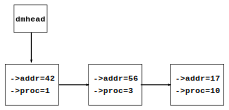
\includegraphics{defer/DemuxList}}
\end{center}
\caption{Pre-BSD Packet Demultiplexing List}
\label{fig:defer:Pre-BSD Packet Demultiplexing List}
\end{figure}

% defer/refcnt.tex

\section{Reference Counting}
\label{sec:defer:Reference Counting}

Reference counting tracks the number of references
to a given object in order to prevent that object from being prematurely
freed.
Although this is a conceptually simple technique, many devils hide in
the details.
After all, if the object was not subject to being prematurely freed,
there would be no need for the reference counter.
But if the object \emph{is} subject to being prematurely freed,
what prevents that object from being freed during
the reference-acquisition process itself?

There are a number of possible answers to this question, including:

\begin{enumerate}
\item	A lock residing outside of the object must be held while
	manipulating the reference count.
	Note that there are a wide variety of types of locks,
	however, pretty much any type will suffice.
\item	The object is created with a non-zero reference count, and new
	references may be acquired only when the current value of
	the reference counter is non-zero.
	Once acquired, a reference may be handed off to some
	other entity.
\item	An existence guarantee is provided for the object, so that
	it cannot be freed during any time interval when some
	entity might be attempting to acquire a reference.
	Existence guarantees are often provided by automatic
	garbage collectors, and, as will be seen in
	Section~\ref{sec:defer:Read-Copy Update (RCU)}, they can
	also be provided by RCU.
\item	A type-safety guarantee is provided for the object, and there
	is in addition some identity check that can be performed once
	the reference is acquired.
	Type-safety guarantees can be provided by special-purpose
	memory allocators, and can also be provided by the
	\url{SLAB_DESTROY_BY_RCU} feature within the Linux kernel,
	again, as will be seen in
	Section~\ref{sec:defer:Read-Copy Update (RCU)}.
\end{enumerate}

Of course, any mechanism that provides existence guarantees
by definition also provides type-safety guarantees.
This section will therefore group the last two answers together under the
rubric of RCU, leaving us with three general categories of
reference-acquisition protection, namely, locking, reference counting,
and RCU.

\QuickQuiz{}
	Why not implement reference-acquisition using
	a simple compare-and-swap operation that only
	acquires a reference if the reference counter is
	non-zero?
\QuickQuizAnswer{
	Although this can resolve the race between the release of
	the last reference and acquisition of a new reference,
	it does absolutely nothing to prevent the data structure
	from being freed and reallocated, possibly as some completely
	different type of structure.
	It is quite likely that the ``simple compare-and-swap
	operation'' would give undefined results if applied to the
	differently typed structure.

	In short, use of atomic operations such as compare-and-swap
	absolutely requires either type-safety or existence guarantees.
} \QuickQuizEnd

\begin{table}
\centering
\begin{tabular}{l||c|c|c}
	& \multicolumn{3}{c}{Release Synchronization} \\
	\cline{2-4}
	Acquisition     &         & Reference &     \\
	Synchronization & Locking & Counting  & RCU \\
	\hline
	\hline
	Locking		& -	  & CAM	      & CA  \\
	\hline
	Reference	& A	  & AM	      & A   \\
	Counting	&  	  &   	      &     \\
	\hline
	RCU		& CA	  & MCA	      & CA  \\
\end{tabular}
\caption{Reference Counting and Synchronization Mechanisms}
\label{tab:defer:Reference Counting and Synchronization Mechanisms}
\end{table}

Given that the key reference-counting issue
is synchronization between acquisition
of a reference and freeing of the object, we have nine possible
combinations of mechanisms, as shown in
Table~\ref{tab:defer:Reference Counting and Synchronization Mechanisms}.
This table
divides reference-counting mechanisms into the following broad categories:
\begin{enumerate}
\item	Simple counting with neither atomic operations, memory
	barriers, nor alignment constraints \makebox{(``-'')}.
\item	Atomic counting without memory barriers (``A'').
\item	Atomic counting, with memory barriers required only on release
	(``AM'').
\item	Atomic counting with a check combined with the atomic acquisition
	operation, and with memory barriers required only on release
	(``CAM'').
\item	Atomic counting with a check combined with the atomic acquisition
	operation (``CA'').
\item	Atomic counting with a check combined with the atomic acquisition
	operation, and with memory barriers also required on acquisition
	(``MCA'').
\end{enumerate}
However, because all Linux-kernel atomic operations that return a
value are defined to contain memory barriers, all release operations
contain memory barriers, and all checked acquisition operations also
contain memory barriers.
Therefore, cases ``CA'' and ``MCA'' are equivalent to ``CAM'', so that
there are sections below for only the first four cases:
\makebox{``-''}, ``A'', ``AM'', and ``CAM''.
The Linux primitives that support reference counting are presented in
Section~\ref{sec:defer:Linux Primitives Supporting Reference Counting}.
Later sections cite optimizations that can improve performance
if reference acquisition and release is very frequent, and the
reference count need be checked for zero only very rarely.

\subsection{Implementation of Reference-Counting Categories}
\label{sec:defer:Implementation of Reference-Counting Categories}

Simple counting protected by locking (\makebox{``-''}) is described in
Section~\ref{sec:defer:Simple Counting},
atomic counting with no memory barriers (``A'') is described in
Section~\ref{sec:defer:Atomic Counting}
atomic counting with acquisition memory barrier (``AM'') is described in
Section~\ref{sec:defer:Atomic Counting With Release Memory Barrier},
and
atomic counting with check and release memory barrier (``CAM'') is described in
Section~\ref{sec:defer:Atomic Counting With Check and Release Memory Barrier}.

\subsubsection{Simple Counting}
\label{sec:defer:Simple Counting}

Simple counting, with neither atomic operations nor memory barriers,
can be used when the reference-counter acquisition and release are
both protected by the same lock.
In this case, it should be clear that the reference count itself
may be manipulated non-atomically, because the lock provides any
necessary exclusion, memory barriers, atomic instructions, and disabling
of compiler optimizations.
This is the method of choice when the lock is required to protect
other operations in addition to the reference count, but where
a reference to the object must be held after the lock is released.
Figure~\ref{fig:defer:Simple Reference-Count API} shows a simple
API that might be used to implement simple non-atomic reference
counting -- although simple reference counting is almost always
open-coded instead.

\begin{figure}[htbp]
{ \scriptsize
\begin{verbatim}
  1 struct sref {
  2   int refcount;
  3 };
  4
  5 void sref_init(struct sref *sref)
  6 {
  7   sref->refcount = 1;
  8 }
  9
 10 void sref_get(struct sref *sref)
 11 {
 12   sref->refcount++;
 13 }
 14
 15 int sref_put(struct sref *sref,
 16              void (*release)(struct sref *sref))
 17 {
 18   WARN_ON(release == NULL);
 19   WARN_ON(release == (void (*)(struct sref *))kfree);
 20
 21   if (--sref->refcount == 0) {
 22     release(sref);
 23     return 1;
 24   }
 25   return 0;
 26 }
\end{verbatim}
}
\caption{Simple Reference-Count API}
\label{fig:defer:Simple Reference-Count API}
\end{figure}

\subsubsection{Atomic Counting}
\label{sec:defer:Atomic Counting}

Simple atomic counting may be used in cases where any CPU acquiring
a reference must already hold a reference.
This style is used when a single CPU creates an object for its
own private use, but must allow other CPU, tasks, timer handlers,
or I/O completion handlers that it later spawns to also access this object.
Any CPU that hands the object off must first acquire a new reference
on behalf of the recipient object.
In the Linux kernel, the \url{kref} primitives are used to implement
this style of reference counting, as shown in
Figure~\ref{fig:defer:Linux Kernel kref API}.

Atomic counting is required
because locking is not used to protect all reference-count operations,
which means that it is possible for two different CPUs to concurrently
manipulate the reference count.
If normal increment and decrement were used, a pair of CPUs might both
fetch the reference count concurrently, perhaps both obtaining
the value ``3''.
If both of them increment their value, they will both obtain ``4'',
and both will store this value back into the counter.
Since the new value of the counter should instead be ``5'', one
of the two increments has been lost.
Therefore, atomic operations must be used both for counter increments
and for counter decrements.

If releases are guarded by locking or RCU,
memory barriers are \emph{not} required, but for different reasons.
In the case of locking, the locks provide any needed memory barriers
(and disabling of compiler optimizations), and the locks also
prevent a pair of releases from running concurrently.
In the case of RCU, cleanup must be deferred until all currently
executing RCU read-side critical sections have completed, and
any needed memory barriers or disabling of compiler optimizations
will be provided by the RCU infrastructure.
Therefore, if two CPUs release the final two references concurrently,
the actual cleanup will be deferred until both CPUs exit their
RCU read-side critical sections.

\QuickQuiz{}
	Why isn't it necessary to guard against cases where one CPU
	acquires a reference just after another CPU releases the last
	reference?
\QuickQuizAnswer{
	Because a CPU must already hold a reference in order
	to legally acquire another reference.
	Therefore, if one CPU releases the last reference,
	there cannot possibly be any CPU that is permitted
	to acquire a new reference.
	This same fact allows the non-atomic check in line~22
	of Figure~\ref{fig:defer:Linux Kernel kref API}.
} \QuickQuizEnd

\begin{figure}[htbp]
{ \scriptsize
\begin{verbatim}
  1 struct kref {
  2   atomic_t refcount;
  3 };
  4
  5 void kref_init(struct kref *kref)
  6 {
  7   atomic_set(&kref->refcount,1);
  8 }
  9
 10 void kref_get(struct kref *kref)
 11 {
 12   WARN_ON(!atomic_read(&kref->refcount));
 13   atomic_inc(&kref->refcount);
 14 }
 15
 16 int kref_put(struct kref *kref,
 17              void (*release)(struct kref *kref))
 18 {
 19   WARN_ON(release == NULL);
 20   WARN_ON(release == (void (*)(struct kref *))kfree);
 21
 22   if ((atomic_read(&kref->refcount) == 1) ||
 23       (atomic_dec_and_test(&kref->refcount))) {
 24     release(kref);
 25     return 1;
 26   }
 27   return 0;
 28 }
\end{verbatim}
}
\caption{Linux Kernel kref API}
\label{fig:defer:Linux Kernel kref API}
\end{figure}

The \url{kref} structure itself, consisting of a single atomic
data item, is shown in lines~1-3 of
Figure~\ref{fig:defer:Linux Kernel kref API}.
The \url{kref_init()} function on lines~5-8 initializes the counter
to the value ``1''.
Note that the \url{atomic_set()} primitive is a simple
assignment, the name stems from the data type of \url{atomic_t}
rather than from the operation.
The \url{kref_init()} function must be invoked during object creation,
before the object has been made available to any other CPU.

The \url{kref_get()} function on lines~10-14 unconditionally atomically
increments the counter.
The \url{atomic_inc()} primitive does not necessarily explicitly
disable compiler
optimizations on all platforms, but the fact that the \url{kref}
primitives are in a separate module and that the Linux kernel build
process does no cross-module optimizations has the same effect.

The \url{kref_put()} function on lines~16-28 checks for the counter having the
value ``1'' on line~22
(in which case no concurrent \url{kref_get()} is permitted),
or if atomically decrementing the counter results in zero on line~23.
In either of these two cases, \url{kref_put()} invokes the
specified \url{release} function and returns ``1'', telling the
caller that cleanup was performed.
Otherwise, \url{kref_put()} returns ``0''.

\QuickQuiz{}
	If the check on line~22 of
	Figure~\ref{fig:defer:Linux Kernel kref API} fails, how
	could the check on line~23 possibly succeed?
\QuickQuizAnswer{
	Suppose that {\tt kref\_put()} is protected by RCU, so
	that two CPUs might be executing line~22 concurrently.
	Both might see the value ``2'', causing both to then
	execute line~23.
	One of the two instances of {\tt atomic\_dec\_and\_test()}
	will decrement the value to zero and thus return 1.
} \QuickQuizEnd

\QuickQuiz{}
	How can it possibly be safe to non-atomically check for equality
	with ``1'' on line~22 of
	Figure~\ref{fig:defer:Linux Kernel kref API}?
\QuickQuizAnswer{
	Remember that it is not legal to call either {\tt kref\_get()}
	or {\tt kref\_put()} unless you hold a reference.
	If the reference count is equal to ``1'', then there
	can't possibly be another CPU authorized to change the
	value of the reference count.
} \QuickQuizEnd

\subsubsection{Atomic Counting With Release Memory Barrier}
\label{sec:defer:Atomic Counting With Release Memory Barrier}

This style of reference is used in the Linux kernel's networking
layer to track the destination caches that are used in packet routing.
The actual implementation is quite a bit more involved; this section
focuses on the aspects of \url{struct} \url{dst_entry} reference-count
handling that matches this use case,
shown in Figure~\ref{fig:defer:Linux Kernel dst-clone API}.

\begin{figure}[htbp]
{ \scriptsize
\begin{verbatim}
  1 static inline
  2 struct dst_entry * dst_clone(struct dst_entry * dst)
  3 {
  4   if (dst)
  5     atomic_inc(&dst->__refcnt);
  6   return dst;
  7 }
  8
  9 static inline
 10 void dst_release(struct dst_entry * dst)
 11 {
 12   if (dst) {
 13     WARN_ON(atomic_read(&dst->__refcnt) < 1);
 14     smp_mb__before_atomic_dec();
 15     atomic_dec(&dst->__refcnt);
 16   }
 17 }
\end{verbatim}
}
\caption{Linux Kernel dst\_clone API}
\label{fig:defer:Linux Kernel dst-clone API}
\end{figure}

The \url{dst_clone()} primitive may be used if the caller
already has a reference to the specified \url{dst_entry},
in which case it obtains another reference that may be handed off
to some other entity within the kernel.
Because a reference is already held by the caller, \url{dst_clone()}
need not execute any memory barriers.
The act of handing the \url{dst_entry} to some other entity might
or might not require a memory barrier, but if such a memory barrier
is required, it will be embedded in the mechanism used to hand the
\url{dst_entry} off.

The \url{dst_release()} primitive may be invoked from any environment,
and the caller might well reference elements of the \url{dst_entry}
structure immediately prior to the call to \url{dst_release()}.
The \url{dst_release()} primitive therefore contains a memory
barrier on line~14 preventing both the compiler and the CPU
from misordering accesses.

Please note that the programmer making use of \url{dst_clone()} and
\url{dst_release()} need not be aware of the memory barriers, only
of the rules for using these two primitives.

\subsubsection{Atomic Counting With Check and Release Memory Barrier}
\label{sec:defer:Atomic Counting With Check and Release Memory Barrier}

The fact that reference-count acquisition can run concurrently
with reference-count release adds further complications.
Suppose that a reference-count release finds that the new
value of the reference count is zero, signalling that it is
now safe to clean up the reference-counted object.
We clearly cannot allow a reference-count acquisition to
start after such clean-up has commenced, so the acquisition
must include a check for a zero reference count.
This check must be part of the atomic increment operation,
as shown below.

\QuickQuiz{}
	Why can't the check for a zero reference count be
	made in a simple ``if'' statement with an atomic
	increment in its ``then'' clause?
\QuickQuizAnswer{
	Suppose that the ``if'' condition completed, finding
	the reference counter value equal to one.
	Suppose that a release operation executes, decrementing
	the reference counter to zero and therefore starting
	cleanup operations.
	But now the ``then'' clause can increment the counter
	back to a value of one, allowing the object to be
	used after it has been cleaned up.
} \QuickQuizEnd

The Linux kernel's \url{fget()} and \url{fput()} primitives
use this style of reference counting.
Simplified versions of these functions are shown in
Figure~\ref{fig:defer:Linux Kernel fget/fput API}.

\begin{figure}[htbp]
{ \scriptsize
\begin{verbatim}
  1 struct file *fget(unsigned int fd)
  2 {
  3   struct file *file;
  4   struct files_struct *files = current->files;
  5
  6   rcu_read_lock();
  7   file = fcheck_files(files, fd);
  8   if (file) {
  9     if (!atomic_inc_not_zero(&file->f_count)) {
 10       rcu_read_unlock();
 11       return NULL;
 12     }
 13   }
 14   rcu_read_unlock();
 15   return file;
 16 }
 17
 18 struct file *
 19 fcheck_files(struct files_struct *files, unsigned int fd)
 20 {
 21   struct file * file = NULL;
 22   struct fdtable *fdt = rcu_dereference((files)->fdt);
 23
 24   if (fd < fdt->max_fds)
 25     file = rcu_dereference(fdt->fd[fd]);
 26   return file;
 27 }
 28
 29 void fput(struct file *file)
 30 {
 31   if (atomic_dec_and_test(&file->f_count))
 32     call_rcu(&file->f_u.fu_rcuhead, file_free_rcu);
 33 }
 34
 35 static void file_free_rcu(struct rcu_head *head)
 36 {
 37   struct file *f;
 38
 39   f = container_of(head, struct file, f_u.fu_rcuhead);
 40   kmem_cache_free(filp_cachep, f);
 41 }
\end{verbatim}
}
\caption{Linux Kernel fget/fput API}
\label{fig:defer:Linux Kernel fget/fput API}
\end{figure}

Line~4 of \url{fget()} fetches the a pointer to the current
process's file-descriptor table, which might well be shared
with other processes.
Line~6 invokes \url{rcu_read_lock()}, which
enters an RCU read-side critical section.
The callback function from any subsequent \url{call_rcu()} primitive
will be deferred until a matching \url{rcu_read_unlock()} is reached
(line~10 or 14 in this example).
Line~7 looks up the file structure corresponding to the file
descriptor specified by the \url{fd} argument, as will be
described later.
If there is an open file corresponding to the specified file descriptor,
then line~9 attempts to atomically acquire a reference count.
If it fails to do so, lines~10-11 exit the RCU read-side critical
section and report failure.
Otherwise, if the attempt is successful, lines~14-15 exit the read-side
critical section and return a pointer to the file structure.

The \url{fcheck_files()} primitive is a helper function for
\url{fget()}.
It uses the \url{rcu_dereference()} primitive to safely fetch an
RCU-protected pointer for later dereferencing (this emits a
memory barrier on CPUs such as DEC Alpha in which data dependencies
do not enforce memory ordering).
Line~22 uses \url{rcu_dereference()} to fetch a pointer to this
task's current file-descriptor table,
and line~24 checks to see if the specified file descriptor is in range.
If so, line~25 fetches the pointer to the file structure, again using
the \url{rcu_dereference()} primitive.
Line~26 then returns a pointer to the file structure or \url{NULL}
in case of failure.

The \url{fput()} primitive releases a reference to a file structure.
Line~31 atomically decrements the reference count, and, if the result
was zero, line~32 invokes the \url{call_rcu()} primitives in order to
free up the file structure (via the \url{file_free_rcu()} function
specified in \url{call_rcu()}'s second argument),
but only after all currently-executing
RCU read-side critical sections complete.
The time period required for all currently-executing RCU read-side
critical sections to complete is termed a ``grace period''.
Note that the \url{atomic_dec_and_test()} primitive contains
a memory barrier.
This memory barrier is not necessary in this example, since the structure
cannot be destroyed until the RCU read-side critical section completes,
but in Linux, all atomic operations that return a result must
by definition contain memory barriers.

Once the grace period completes, the \url{file_free_rcu()} function
obtains a pointer to the file structure on line~39, and frees it
on line~40.

This approach is also used by Linux's virtual-memory system,
see \url{get_page_unless_zero()} and \url{put_page_testzero()} for
page structures as well as \url{try_to_unuse()} and \url{mmput()}
for memory-map structures.

\subsection{Linux Primitives Supporting Reference Counting}
\label{sec:defer:Linux Primitives Supporting Reference Counting}

The Linux-kernel primitives used in the above examples are
summarized in the following list.
\IfInBook{}{The RCU primitives may be unfamiliar to some readers,
	    so a brief overview with citations is included in
	    Section~\ref{sec:defer:Background on RCU}.}

\begin{itemize}
\item	{\tt atomic\_t}~~
	Type definition for 32-bit quantity to be manipulated atomically.
\item	{\tt void atomic\_dec(atomic\_t *var);}~~
	Atomically decrements the referenced variable without necessarily
	issuing a memory barrier or disabling compiler optimizations.
\item	{\tt int atomic\_dec\_and\_test(atomic\_t *var);}~~
	Atomically decrements the referenced variable, returning
	TRUE if the result is zero.
	Issues a memory barrier and disables compiler optimizations that
	might otherwise move memory references across this primitive.
\item	{\tt void atomic\_inc(atomic\_t *var);}~~
	Atomically increments the referenced variable without necessarily
	issuing a memory barrier or disabling compiler optimizations.
\item	{\tt int atomic\_inc\_not\_zero(atomic\_t *var);}~~
	Atomically increments the referenced variable, but only if the
	value is non-zero, and returning TRUE if the increment occurred.
	Issues a memory barrier and disables compiler optimizations that
	might otherwise move memory references across this primitive.
\item	{\tt int atomic\_read(atomic\_t *var);}~~
	Returns the integer value of the referenced variable.
	This is not an atomic operation, and it neither issues memory
	barriers nor disables compiler optimizations.
\item	{\tt void atomic\_set(atomic\_t *var, int val);}~~
	Sets the value of the referenced atomic variable to ``val''.
	This is not an atomic operation, and it neither issues memory
	barriers nor disables compiler optimizations.
\item	{\tt void call\_rcu(struct rcu\_head *head, void (*func)(struct rcu\_head *head));}~~
	Invokes \url{func(head)} some time after all currently executing RCU
	read-side critical sections complete, however, the \url{call_rcu()}
	primitive returns immediately.
	Note that \url{head} is normally a field within an RCU-protected
	data structure, and that \url{func} is normally a function that
	frees up this data structure.
	The time interval between the invocation of \url{call_rcu()} and
	the invocation of \url{func} is termed a ``grace period''.
	Any interval of time containing a grace period is itself a
	grace period.
\item	{\tt type *container\_of(p, type, f);}~~
	Given a pointer ``p'' to a field ``f'' within a structure
	of the specified type, return a pointer to the structure.
\item	{\tt void rcu\_read\_lock(void);}~~
	Marks the beginning of an RCU read-side critical section.
\item	{\tt void rcu\_read\_unlock(void);}~~
	Marks the end of an RCU read-side critical section.
	RCU read-side critical sections may be nested.
\item	{\tt void smp\_mb\_\_before\_atomic\_dec(void);}~~
	Issues a memory barrier and disables code-motion compiler
	optimizations only if the platform's \url{atomic_dec()}
	primitive does not already do so.
\item	{\tt struct rcu\_head}~~
	A data structure used by the RCU infrastructure to track
	objects awaiting a grace period.
	This is normally included as a field within an RCU-protected
	data structure.
\end{itemize}

\subsection{Counter Optimizations}
\label{sec:defer:Counter Optimizations}

In some cases where increments and decrements are common, but checks
for zero are rare, it makes sense to maintain per-CPU or per-task
counter.
\IfInBook{See Appendix~\ref{app:rcuimpl:Sleepable RCU Implementation}
	  for an example of this technique.}{
	  See the paper on sleepable read-copy update
	  (SRCU) for an example of this technique~\cite{PaulEMcKenney2006c}.}
% @@@ need a section or chapter on counting...
This approach eliminates the need for atomic instructions or memory
barriers on the increment and decrement primitives, but still requires
that code-motion compiler optimizations be disabled.
In addition, the primitives such as \url{synchronize_srcu()}
that check for the aggregate reference
count reaching zero can be quite slow.
This underscores the fact that these techniques are designed
for situations where the references are frequently acquired and
released, but where it is rarely necessary to check for a zero
reference count.

% defer/hazptr.tex
% Can I hazptr cheezeberger?

\section{Hazard Pointers}
\label{sec:defer:Hazard Pointers}

One way of avoiding problems with concurrent reference counting
is to implement the reference counters
inside out, that is, rather than incrementing an integer stored in the
data element, instead store a pointer to that data element in
per-CPU (or per-thread) lists.
Each element of these lists is called a
\emph{hazard pointer}~\cite{MagedMichael04a}.\footnote{
	Also independently invented by others~\cite{HerlihyLM02}.}
The value of a given data element's ``virtual reference counter'' can
then be obtained by counting the number of hazard pointers referencing
that element.
Therefore, if that element has been rendered inaccessible to readers,
and there are no longer any hazard pointers referencing it, that element
may safely be freed.

{ \scriptsize
\begin{verbbox}
 1 int hp_store(void **p, void **hp)
 2 {
 3   void *tmp;
 4 
 5   tmp = ACCESS_ONCE(*p);
 6   ACCESS_ONCE(*hp) = tmp;
 7   smp_mb();
 8   if (tmp != ACCESS_ONCE(*p) ||
 9       tmp == HAZPTR_POISON) {
10     ACCESS_ONCE(*hp) = NULL;
11     return 0;
12   }
13   return 1;
14 }
15 
16 void hp_erase(void **hp)
17 {
18   smp_mb();
19   ACCESS_ONCE(*hp) = NULL;
20   hp_free(hp);
21 }
\end{verbbox}
}
\begin{figure}[btp]
\centering
\theverbbox
\caption{Hazard-Pointer Storage and Erasure}
\label{fig:defer:Hazard-Pointer Storage and Erasure}
\end{figure}

Of course, this means that hazard-pointer acquisition must be carried
out quite carefully in order to avoid destructive races with concurrent
deletion.
One implementation is shown in
Figure~\ref{fig:defer:Hazard-Pointer Storage and Erasure},
which shows \co{hp_store()} on lines~1-13 and \co{hp_erase()} on
lines~15-20.
The \co{smp_mb()} primitive will be described in detail in
Section~\ref{sec:advsync:Memory Barriers}, but may be ignored for
the purposes of this brief overview.

The \co{hp_store()} function records a hazard pointer at \co{hp} for the data
element whose pointer is referenced by \co{p}, while checking for
concurrent modifications.
If a concurrent modification occurred, \co{hp_store()} refuses to record
a hazard pointer, and returns zero to indicate that the caller must
restart its traversal from the beginning.
Otherwise, \co{hp_store()} returns one to indicate that it successfully
recorded a hazard pointer for the data element.

\QuickQuiz{}
	Why does \co{hp_store()} in
	Figure~\ref{fig:defer:Hazard-Pointer Storage and Erasure}
	take a double indirection to the data element?
	Why not \co{void *} instead of \co{void **}?
\QuickQuizAnswer{
	Because \co{hp_record()} must check for concurrent modifications.
	To do that job, it needs a pointer to a pointer to the element,
	so that it can check for a modification to the pointer to the
	element.
} \QuickQuizEnd

\QuickQuiz{}
	Why does \co{hp_store()}'s caller need to restart its
	traversal from the beginning in case of failure?
	Isn't that inefficient for large data structures?
\QuickQuizAnswer{
	It might be inefficient in some sense, but the fact is that
	such restarting is absolutely required for correctness.
	To see this, consider a hazard-pointer-protected linked list
	containing elements~A, B, and~C that is subjecte to the
	following sequence of events:

	\begin{enumerate}
	\item	Thread~0 stores a hazard pointer to element~B
		(having presumably traversed to element~B from element~A).
	\item	Thread~1 removes element~B from the list, which sets
		the pointer from element~B to element~C to a special
		\co{HAZPTR_POISON} value in order to mark the deletion.
		Because Thread~0 has a hazard pointer to element~B,
		it cannot yet be freed.
	\item	Thread~1 removes element~C from the list.
		Because there are no hazard pointers referencing element~C,
		it is immediately freed.
	\item	Thread~0 attempts to acquire a hazard pointer to
		now-removed element~B's successor, but sees the
		\co{HAZPTR_POISON} value, and thus returns zero,
		forcing the caller to restart its traversal from the
		beginning of the list.
	\end{enumerate}

	Which is a very good thing, because otherwise Thread~0 would
	have attempted to access the now-freed element~C,
	which might have resulted in arbitrarily horrible
	memory corruption, especially if the memory for
	element~C had since been re-allocated for some other
	purpose.

	All that aside, please understand that hazard pointers's
	restarting allows it to maintain a minimal memory footprint.
	Any object not currently referenced by some hazard pointer
	may be immediately freed.
	In contrast,
	Section~\ref{sec:defer:Read-Copy Update (RCU)}
	will discuss a mechanism that avoids read-side retries
	(and minimizes read-side overhead), but has a much larger
	memory footprint.
} \QuickQuizEnd

\QuickQuiz{}
	Given that papers on hazard pointers use the bottom bits
	of each pointer to mark deleted elements, what is up with
	\co{HAZPTR_POISON}?
\QuickQuizAnswer{
	The published implementations of hazard pointers used
	non-blocking synchronization techniques for insertion
	and deletion.
	These techniques require that readers traversing the
	data structure ``help'' updaters complete their updates,
	which in turn means that readers need to look at the successor
	of a deleted element.

	In contrast, we will be using locking to synchronize updates,
	which does away with the need for readers to help updaters
	complete their updates, which in turn allows us to leave
	pointers' bottom bits alone.
	This approach allows read-side code to be simpler and faster.
} \QuickQuizEnd

Because algorithms using hazard pointers might be restarted at any
step of their traversal through the data structure, such algorithms
must typically take care to avoid making any changes to the data
structure until after they have acquired all relevant hazard pointers.

\QuickQuiz{}
	But don't these restrictions on hazard pointers also apply
	to other forms of reference counting?
\QuickQuizAnswer{
	These restrictions apply only to reference-counting mechanisms whose
	reference acquisition can fail.
} \QuickQuizEnd

These restrictions result in great benefits to readers, courtesy of the
fact that the hazard pointers are stored local to each CPU/thread,
which in turn allows traversals of the data structures themselves to
be carried out in a completely read-only fashion.
Referring back to
Figure~\ref{fig:count:Optimization and the Four Parallel-Programming Tasks}
on
page~\pageref{fig:count:Optimization and the Four Parallel-Programming Tasks},
hazard pointers enable the CPU caches to do resource replication, which
in turn allows weakening of the parallel-access-control mechanism,
thus boosting performance and scalability.
Performance comparisons with other mechanisms may be found in
Chapter~\ref{chp:Data Structures}
and in other publications~\cite{ThomasEHart2007a,McKenney:2013:SDS:2483852.2483867,MagedMichael04a}.

{ \scriptsize
\begin{verbbox}
 1 struct route_entry {
 2   struct hazptr_head hh;
 3   struct route_entry *re_next;
 4   unsigned long addr;
 5   unsigned long iface;
 6   int re_freed;
 7 };
 8 struct route_entry route_list;
 9 DEFINE_SPINLOCK(routelock);
10 hazard_pointer __thread *my_hazptr;
11
12 unsigned long route_lookup(unsigned long addr)
13 {
14   int offset = 0;
15   struct route_entry *rep;
16   struct route_entry **repp;
17
18 retry:
19   repp = &route_list.re_next;
20   do {
21     rep = ACCESS_ONCE(*repp);
22     if (rep == NULL)
23       return ULONG_MAX;
24     if (rep == (struct route_entry *)HAZPTR_POISON)
25       goto retry;
26     my_hazptr[offset].p = &rep->hh;
27     offset = !offset;
28     smp_mb();
29     if (ACCESS_ONCE(*repp) != rep)
30       goto retry;
31     repp = &rep->re_next;
32   } while (rep->addr != addr);
33   if (ACCESS_ONCE(rep->re_freed))
34     abort();
35   return rep->iface;
36 }
\end{verbbox}
}
\begin{figure}[tbp]
\centering
\theverbbox
\caption{Hazard-Pointer Pre-BSD Routing Table Lookup}
\label{fig:defer:Hazard-Pointer Pre-BSD Routing Table Lookup}
\end{figure}

{ \scriptsize
\begin{verbbox}
 1 int route_add(unsigned long addr,
 2               unsigned long interface)
 3 {
 4   struct route_entry *rep;
 5
 6   rep = malloc(sizeof(*rep));
 7   if (!rep)
 8     return -ENOMEM;
 9   rep->addr = addr;
10   rep->iface = interface;
11   rep->re_freed = 0;
12   spin_lock(&routelock);
13   rep->re_next = route_list.re_next;
14   route_list.re_next = rep;
15   spin_unlock(&routelock);
16   return 0;
17 }
18
19 int route_del(unsigned long addr)
20 {
21   struct route_entry *rep;
22   struct route_entry **repp;
23
24   spin_lock(&routelock);
25   repp = &route_list.re_next;
26   for (;;) {
27     rep = *repp;
28     if (rep == NULL)
29       break;
30     if (rep->addr == addr) {
31       *repp = rep->re_next;
32       rep->re_next =
33           (struct route_entry *)HAZPTR_POISON;
34       spin_unlock(&routelock);
35       hazptr_free_later(&rep->hh);
36       return 0;
37     }
38     repp = &rep->re_next;
39   }
40   spin_unlock(&routelock);
41   return -ENOENT;
42 }
\end{verbbox}
}
\begin{figure}[tbp]
\centering
\theverbbox
\caption{Hazard-Pointer Pre-BSD Routing Table Add/Delete}
\label{fig:defer:Hazard-Pointer Pre-BSD Routing Table Add/Delete}
\end{figure}

The Pre-BSD routing example can use hazard pointers as shown in
Figure~\ref{fig:defer:Hazard-Pointer Pre-BSD Routing Table Lookup}
for data structures and \co{route_lookup()}, and in
Figure~\ref{fig:defer:Hazard-Pointer Pre-BSD Routing Table Add/Delete}
for \co{route_add()} and \co{route_del()}
(\path{route_hazptr.c}).
As with reference counting, the hazard-pointers implementation
is quite similar to the sequential algorithm shown in
Figure~\ref{fig:defer:Sequential Pre-BSD Routing Table}
on
page~\pageref{fig:defer:Sequential Pre-BSD Routing Table},
so only differences will be discussed.

Starting with
Figure~\ref{fig:defer:Hazard-Pointer Pre-BSD Routing Table Lookup},
line~2 shows the \co{->hh} field used to queue objects pending
hazard-pointer free,
line~6 shows the \co{->re_freed} field used to detect use-after-free bugs,
and lines~24-30 attempt to acquire a hazard pointer, branching
to line~18's \co{retry} label on failure.

In
Figure~\ref{fig:defer:Hazard-Pointer Pre-BSD Routing Table Add/Delete},
line~11 initializes \co{->re_freed},
lines~32 and~33 poison the \co{->re_next} field of the newly removed
object, and
line~35 passes that object to the hazard pointers's
\co{hazptr_free_later()} function, which will free that object once it
is safe to do so.
The spinlocks work the same as in
Figure~\ref{fig:defer:Reference-Counted Pre-BSD Routing Table Add/Delete}.

\begin{figure}[tb]
\centering
\resizebox{2.5in}{!}{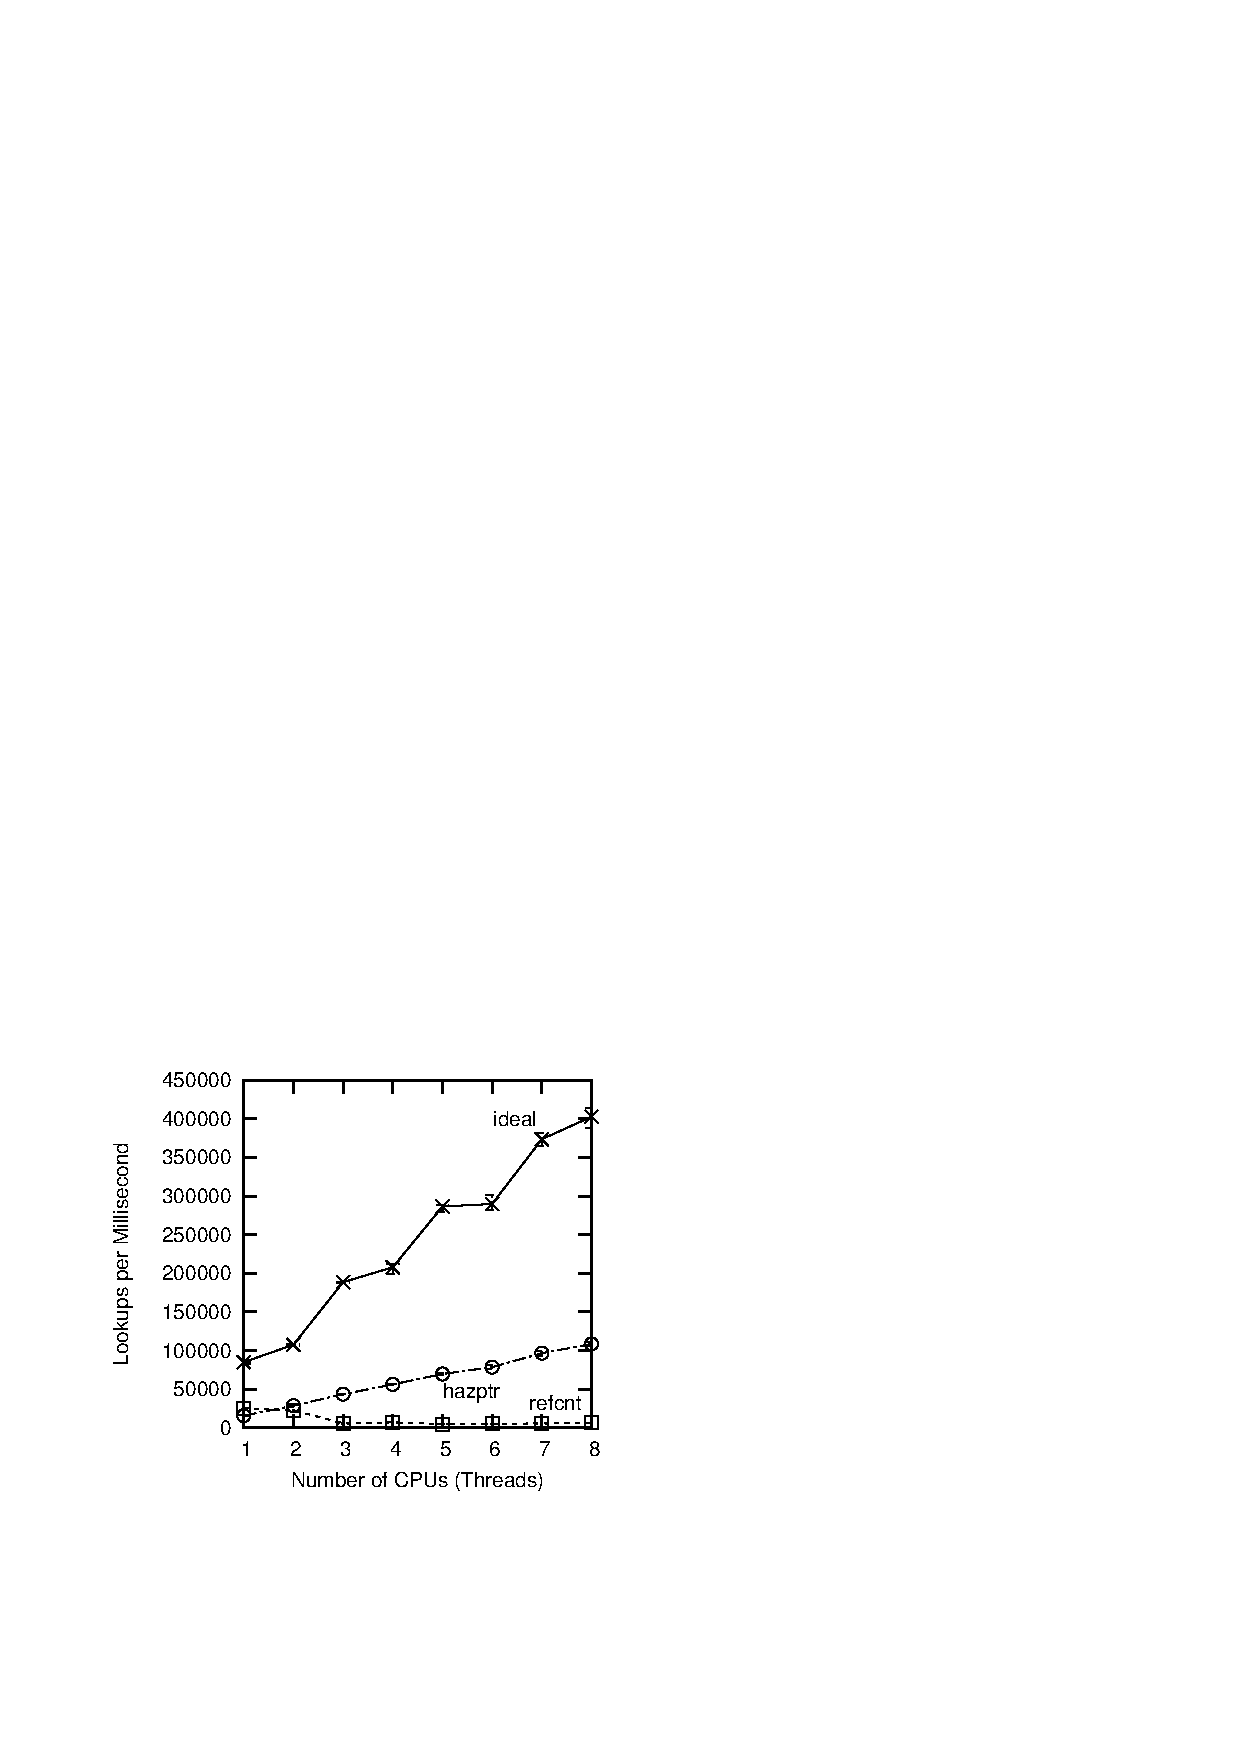
\includegraphics{CodeSamples/defer/perf-hazptr}}
\caption{Pre-BSD Routing Table Protected by Hazard Pointers}
\label{fig:defer:Pre-BSD Routing Table Protected by Hazard Pointers}
\end{figure}

Figure~\ref{fig:defer:Pre-BSD Routing Table Protected by Hazard Pointers}
shows the hazard-pointers-protected Pre-BSD routing algorithm's
performance on the same read-only workload as for
Figure~\ref{fig:defer:Pre-BSD Routing Table Protected by Reference Counting}.
Although hazard pointers scales much better than does reference counting,
hazard pointers still require readers to do writes to shared
memory (albeit with much improved locality of reference),
and also require a full memory barrier and retry check for each
object traversed.
Therefore, hazard pointers's performance is far short of ideal.
On the other hand, hazard pointers do operate correctly for workloads
involving concurrent updates.

\QuickQuiz{}
	The paper ``Structured Deferral: Synchronization via
	Procrastination''~\cite{McKenney:2013:SDS:2483852.2483867}
	shows that hazard pointers have near-ideal performance.
	Whatever happened in
	Figure~\ref{fig:defer:Pre-BSD Routing Table Protected by Hazard Pointers}???
\QuickQuizAnswer{
	First,
	Figure~\ref{fig:defer:Pre-BSD Routing Table Protected by Hazard Pointers}
	has a linear y-axis, while most of the graphs in the
	``Structured Deferral'' paper have logscale y-axes.
	Next, that paper uses hash tables, while
	Figure~\ref{fig:defer:Pre-BSD Routing Table Protected by Hazard Pointers}'s
	uses a simple linked list.
	Finally, that paper used a larger and older x86 system, while
	a newer but smaller system that was used to generate the data
	shown in
	Figure~\ref{fig:defer:Pre-BSD Routing Table Protected by Hazard Pointers}.
} \QuickQuizEnd

The next section attempts to improve on hazard pointers by using
sequence locks, which avoid both read-side writes and per-object memory
barriers.

% defer/seqlock.tex

\section{Sequence Locks}
\label{sec:defer:Sequence Locks}

\begin{figure}[tb]
\begin{center}
\resizebox{3in}{!}{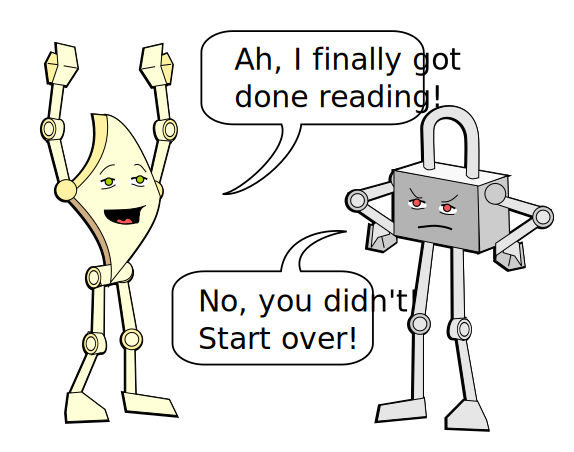
\includegraphics{cartoons/r-2014-Start-over}}
\end{center}
\caption{Reader And Uncooperative Sequence Lock}
\label{fig:defer:Reader And Uncooperative Sequence Lock}
\end{figure}

Sequence locks are used in the Linux kernel for read-mostly data that
must be seen in a consistent state by readers.
However, unlike reader-writer locking, readers do not exclude writers.
Instead, like hazard pointers, sequence locks force readers to
\emph{retry} an operation if they detect activity from a concurrent writer.
As can be seen from
Figure~\ref{fig:defer:Reader And Uncooperative Sequence Lock},
it is important to design code using sequence locks so that readers
very rarely need to retry.

\QuickQuiz{}
	Why isn't this sequence-lock discussion in Chapter~\ref{chp:Locking},
	you know, the one on \emph{locking}?
\QuickQuizAnswer{
	The sequence-lock mechanism is really a combination of two
	separate synchronization mechanisms, sequence counts and
	locking.
	In fact, the sequence-count mechanism is available separately
	in the Linux kernel via the
	\co{write_seqcount_begin()} and \co{write_seqcount_end()}
	primitives.

	However, the combined \co{write_seqlock()} and
	\co{write_sequnlock()} primitives are used much more heavily
	in the Linux kernel.
	More importantly, many more people will understand what you
	mean if you say ``sequence lock'' than if you say
	``sequence count''.

	So this section is entitled ``Sequence Locks'' so that people
	will understand what it is about just from the title, and
	it appears in the ``Deferred Processing'' because (1) of the
	emphasis on the ``sequence count'' aspect of ``sequence locks''
	and (2) because a ``sequence lock'' is much more than merely
	a lock.
} \QuickQuizEnd

{ \scriptsize
\begin{verbbox}
  1 do {
  2   seq = read_seqbegin(&test_seqlock);
  3   /* read-side access. */
  4 } while (read_seqretry(&test_seqlock, seq));
\end{verbbox}
}
\begin{figure}[bp]
\centering
\theverbbox
\caption{Sequence-Locking Reader}
\label{fig:defer:Sequence-Locking Reader}
\end{figure}

{ \scriptsize
\begin{verbbox}
  1 write_seqlock(&test_seqlock);
  2 /* Update */
  3 write_sequnlock(&test_seqlock);
\end{verbbox}
}
\begin{figure}[bp]
\centering
\theverbbox
\caption{Sequence-Locking Writer}
\label{fig:defer:Sequence-Locking Writer}
\end{figure}

The key component of sequence locking is the sequence number, which has
an even value in the absence of writers and an odd value if there
is an update in progress.
Readers can then snapshot the value before and after each access.
If either snapshot has an odd value, or if the two snapshots differ,
there has been a concurrent update, and the reader must discard
the results of the access and then retry it.
Readers use the \co{read_seqbegin()} and \co{read_seqretry()}
functions, as shown in Figure~\ref{fig:defer:Sequence-Locking Reader},
when accessing data protected by a sequence lock.
Writers must increment the value before and after each update,
and only one writer is permitted at a given time.
Writers use the \co{write_seqlock()} and \co{write_sequnlock()}
functions, as shown in Figure~\ref{fig:defer:Sequence-Locking Writer},
when updating data protected by a sequence lock.

Sequence-lock-protected data can have an arbitrarily large number of
concurrent readers, but only one writer at a time.
Sequence locking is used in the Linux kernel to protect calibration
quantities used for timekeeping.
It is also used in pathname traversal to detect concurrent rename operations.

\QuickQuiz{}
	Can you use sequence locks as the only synchronization
	mechanism protecting a linked list supporting concurrent
	addition, deletion, and search?
\QuickQuizAnswer{
	One trivial way of accomplishing this is to surround all
	accesses, including the read-only accesses, with
	\co{write_seqlock()} and \co{write_sequnlock()}.
	Of course, this solution also prohibits all read-side
	parallelism, and furthermore could just as easily be implemented
	using simple locking.

	If you do come up with a solution that uses \co{read_seqbegin()}
	and \co{read_seqretry()} to protect read-side accesses, make
	sure that you correctly handle the following sequence of events:

	\begin{enumerate}
	\item	CPU~0 is traversing the linked list, and picks up a pointer
		to list element~A.
	\item	CPU~1 removes element~A from the list and frees it.
	\item	CPU~2 allocates an unrelated data structure, and gets
		the memory formerly occupied by element~A.
		In this unrelated data structure, the memory previously
		used for element~A's \co{->next} pointer is now occupied
		by a floating-point number.
	\item	CPU~0 picks up what used to be element~A's \co{->next}
		pointer, gets random bits, and therefore gets a
		segmentation fault.
	\end{enumerate}

	One way to protect against this sort of problem requires use
	of ``type-safe memory'', which will be discussed in
	Section~\ref{sec:defer:RCU is a Way of Providing Type-Safe Memory}.
	But in that case, you would be using some other synchronization
	mechanism in addition to sequence locks!
} \QuickQuizEnd

{ \scriptsize
\begin{verbbox}
  1 typedef struct {
  2   unsigned long seq;
  3   spinlock_t lock;
  4 } seqlock_t;
  5 
  6 static void seqlock_init(seqlock_t *slp)
  7 {
  8   slp->seq = 0;
  9   spin_lock_init(&slp->lock);
 10 }
 11 
 12 static unsigned long read_seqbegin(seqlock_t *slp)
 13 {
 14   unsigned long s;
 15 
 16 repeat:
 17   s = ACCESS_ONCE(slp->seq);
 18   smp_mb();
 19   if (unlikely(s & 1))
 20     goto repeat;
 21   return s;
 22 }
 23 
 24 static int read_seqretry(seqlock_t *slp,
 25                          unsigned long oldseq)
 26 {
 27   unsigned long s;
 28 
 29   smp_mb();
 30   s = ACCESS_ONCE(slp->seq);
 31   return s != oldseq;
 32 }
 33 
 34 static void write_seqlock(seqlock_t *slp)
 35 {
 36   spin_lock(&slp->lock);
 37   ++slp->seq;
 38   smp_mb();
 39 }
 40 
 41 static void write_sequnlock(seqlock_t *slp)
 42 {
 43   smp_mb();
 44   ++slp->seq;
 45   spin_unlock(&slp->lock);
 46 }
\end{verbbox}
}
\begin{figure}[bp]
\centering
\theverbbox
\caption{Sequence-Locking Implementation}
\label{fig:defer:Sequence-Locking Implementation}
\end{figure}

A simple implementation of sequence locks is shown in
Figure~\ref{fig:defer:Sequence-Locking Implementation}
(\co{seqlock.h}).
The \co{seqlock_t} data structure is shown on lines~1-4, and contains
the sequence number along with a lock to serialize writers.
Lines~6-10 show \co{seqlock_init()}, which, as the name indicates,
initializes a \co{seqlock_t}.

Lines~12-22 show \co{read_seqbegin()}, which begins a sequence-lock
read-side critical section.
Line~17 takes a snapshot of the sequence counter, and line~18 orders
this snapshot operation before the caller's critical section.
Line~19 checks to see if the snapshot is odd, indicating that there
is a concurrent writer, and, if so, line~20 jumps back to the beginning.
Otherwise, line~21 returns the value of the snapshot, which the caller
will pass to a later call to \co{read_seqretry()}.

\QuickQuiz{}
	Why bother with the check on line~19 of
	\co{read_seqbegin()} in
	Figure~\ref{fig:defer:Sequence-Locking Implementation}?
	Given that a new writer could begin at any time, why not
	simply incorporate the check into line~31 of
	\co{read_seqretry()}?
\QuickQuizAnswer{
	That would be a legitimate implementation.
	However, it would not save anything to move the check down
	to \co{read_seqretry()}: There would be roughly the same number
	of instructions.
	Furthermore, the reader's accesses from its doomed read-side
	critical section could inflict overhead on the writer in
	the form of cache misses.
	We can avoid these cache misses by placing the check in
	\co{read_seqbegin()} as shown on line~19 of
	Figure~\ref{fig:defer:Sequence-Locking Implementation}.
} \QuickQuizEnd

Lines~24-32 show \co{read_seqretry()}, which returns true if there
were no writers present since the time of the corresponding
call to \co{read_seqbegin()}.
Line~29 orders the caller's prior critical section before line~30's
fetch of the new snapshot of the sequence counter.
Finally, line~31 checks that the sequence counter has not changed,
in other words, that there has been no writer, and returns true if so.

\QuickQuiz{}
	Why is the \co{smp_mb()} on line~29 of
	Figure~\ref{fig:defer:Sequence-Locking Implementation}
	needed?
\QuickQuizAnswer{
	If it was omitted, both the compiler and the CPU would be
	within their rights to move the critical section preceding
	the call to \co{read_seqretry()} down below this function.
	This would prevent the sequence lock from protecting the
	critical section.
	The \co{smp_mb()} primitive prevents such reordering.
} \QuickQuizEnd

\QuickQuiz{}
	Can't weaker memory barriers be used in the code in
	Figure~\ref{fig:defer:Sequence-Locking Implementation}?
\QuickQuizAnswer{
	In older versions of the Linux kernel, no.

	In very new versions of the Linux kernel, line~17 could use
	\co{smp_load_acquire()} instead of \co{ACCESS_ONCE()}, which
	in turn would allow the \co{smp_mb()} on line~18 to be dropped.
	Similarly, line~44 could use an \co{smp_store_release()}, for
	example, as follows: \\
	\co{smp_store_release(&slp->seq, ACCESS_ONCE(slp->seq) + 1);} \\
	This would allow the \co{smp_mb()} on line~43 to be dropped.
} \QuickQuizEnd

\QuickQuiz{}
	What prevents sequence-locking updaters from starving readers?
\QuickQuizAnswer{
	Nothing.
	This is one of the weaknesses of sequence locking, and as a
	result, you should use sequence locking only in read-mostly
	situations.
	Unless of course read-side starvation is acceptable in your
	situation, in which case, go wild with the sequence-locking updates!
} \QuickQuizEnd

Lines~34-39 show \co{write_seqlock()}, which simply acquires the lock,
increments the sequence number, and executes a memory barrier to ensure
that this increment is ordered before the caller's critical section.
Lines~41-46 show \co{write_sequnlock()}, which executes a memory barrier
to ensure that the caller's critical section is ordered before the
increment of the sequence number on line~44, then releases the lock.

\QuickQuiz{}
	What if something else serializes writers, so that the lock
	is not needed?
\QuickQuizAnswer{
	In this case, the \co{->lock} field could be omitted, as it
	is in \co{seqcount_t} in the Linux kernel.
} \QuickQuizEnd

\QuickQuiz{}
	Why isn't \co{seq} on line~2 of
	Figure~\ref{fig:defer:Sequence-Locking Implementation}
	\co{unsigned} rather than \co{unsigned long}?
	After all, if \co{unsigned} is good enough for the Linux
	kernel, shouldn't it be good enough for everyone?
\QuickQuizAnswer{
	Not at all.
	The Linux kernel has a number of special attributes that allow
	it to ignore the following sequence of events:
	\begin{enumerate}
	\item	Thread~0 executes \co{read_seqbegin()}, picking up
		\co{->seq} in line~17, noting that the value is even,
		and thus returning to the caller.
	\item	Thread~0 starts executing its read-side critical section,
		but is then preempted for a long time.
	\item	Other threads repeatedly invoke \co{write_seqlock()} and
		\co{write_sequnlock()}, until the value of \co{->seq}
		overflows back to the value that Thread~0 fetched.
	\item	Thread~0 resumes execution, completing its read-side
		critical section with inconsistent data.
	\item	Thread~0 invokes \co{read_seqretry()}, which incorrectly
		concludes that Thread~0 has seen a consistent view of
		the data protected by the sequence lock.
	\end{enumerate}

	The Linux kernel uses sequence locking for things that are
	updated rarely, with time-of-day information being a case
	in point.
	This information is updated at most once per millisecond,
	so that seven weeks would be required to overflow the counter.
	If a kernel thread was preempted for seven weeks, the Linux
	kernel's soft-lockup code would be emitting warnings every two
	minutes for that entire time.

	In contrast, with a 64-bit counter, more than five centuries
	would be required to overflow, even given an update every
	\emph{nano}second.
	Therefore, this implementation uses a type for \co{->seq}
	that is 64 bits on 64-bit systems.
} \QuickQuizEnd

Both the read-side and write-side critical sections of a sequence lock
can be thought of as transactions, and sequence locking therefore
can be thought of as a limited form of transactional memory, which
will be discussed in Section~\ref{sec:future:Transactional Memory}.
The limitations of sequence locking are: (1)~Sequence locking restricts
updates and (2)~sequence locking does not permit traversal of pointers
to objects that might be freed by updaters.
These limitations are of course overcome by transactional memory, but
can also be overcome by combining other synchronization primitives
with sequence locking.

Sequence locks allow writers to defer readers, but not vice versa.
This can result in unfairness and even starvation
in writer-heavy workloads.
On the other hand, in the absence of writers, sequence-lock readers are
reasonably fast and scale linearly.
It is only human to want the best of both worlds: fast readers without
the possibility of read-side failure, let alone starvation.
In addition, it would also be nice to overcome sequence locking's limitations
with pointers.
The following section presents a synchronization mechanism with exactly
these properties.

% rcu.tex
% SPDX-License-Identifier: CC-BY-SA-3.0

\section{Read-Copy Update (RCU)}
\label{sec:defer:Read-Copy Update (RCU)}

This section covers RCU from a number of different perspectives.
Section~\ref{sec:defer:Introduction to RCU} provides the classic
introduction to RCU,
Section~\ref{sec:defer:RCU Fundamentals} covers fundamental RCU
concepts,
Section~\ref{sec:defer:RCU Usage} introduces some common uses of RCU,
Section~\ref{sec:defer:RCU Linux-Kernel API} presents the Linux-kernel
API,
Section~\ref{sec:defer:``Toy'' RCU Implementations} covers a sequence
of ``toy'' implementations of user-level RCU,
and finally
Section~\ref{sec:defer:RCU Exercises} provides some RCU exercises.

% defer/rcuintro.tex

\subsection{Introduction to RCU}
\label{sec:defer:Introduction to RCU}

The approaches discussed in the preceding sections have provided
some scalability but decidedly non-ideal performance for the
Pre-BSD routing table.
It would be nice if the overhead of Pre-BSD lookups was the same as
that of a single-threaded lookup, so that the parallel lookups would
execute the same sequence of assembly language instructions as would a
single-threaded lookup.
Although this is a nice goal, it does raise some serious implementability
questions.
But let's see what happens if we try, treating insertion and deletion
separately.

\begin{figure}[tb]
\centering
\resizebox{3in}{!}{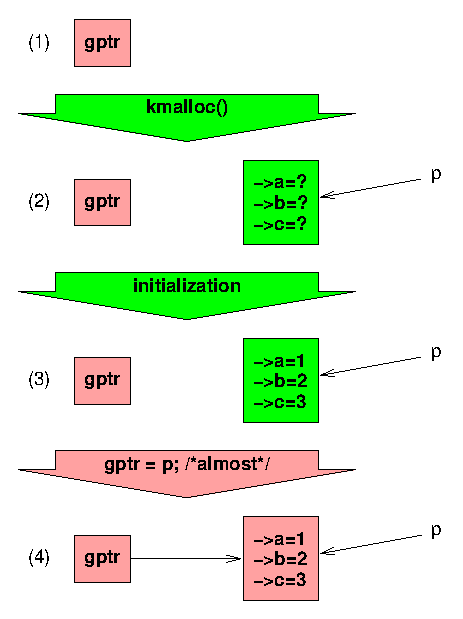
\includegraphics{defer/RCUListInsertClassic}}
\caption{Insertion With Concurrent Readers}
\label{fig:defer:Insertion With Concurrent Readers}
\end{figure}

A classic approach for insertion is shown in
Figure~\ref{fig:defer:Insertion With Concurrent Readers}.
The first row shows the default state, with \co{gptr} equal to \co{NULL}.
In the second row, we have allocated a structure which is uninitialized,
as indicated by the question marks.
In the third row, we have initialized the structure.
Next, we assign \co{gptr} to reference this new element.\footnote{
	On many computer systems, simple assignment is insufficient
	due to interference from both the compiler and the CPU.
	These issues will be covered in
	Section~\ref{sec:defer:RCU Fundamentals}.}
On modern general-purpose systems, this assignment is atomic in the
sense that concurrent readers will see either a \co{NULL} pointer
or a pointer to the new structure \co{p}, but not some mash-up
containing bits from both values.
Each reader is therefore guaranteed to either get the
default value of \co{NULL} or to get the newly installed
non-default values, but either way each reader will see
a consistent result.
Even better, readers need not use any expensive synchronization
primitives, so this approach is quite suitable for real-time use.\footnote{
	Again, on many computer systems, additional work is required
	to prevent interference from the compiler, and, on DEC Alpha
	systems, the CPU as well.
	This will be covered in
	Section~\ref{sec:defer:RCU Fundamentals}.}

\begin{figure}[tb]
\centering
\resizebox{3in}{!}{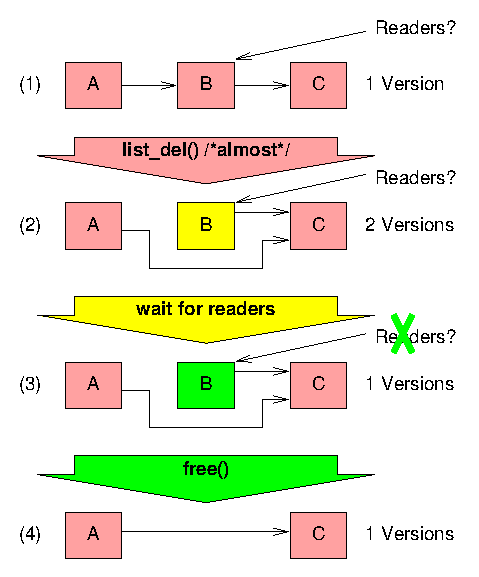
\includegraphics{defer/RCUListDeleteClassic}}
\caption{Deletion From Linked List With Concurrent Readers}
\label{fig:defer:Deletion From Linked List With Concurrent Readers}
\end{figure}

But sooner or later, it will be necessary to remove data that is
being referenced by concurrent readers.
Let us move to a more complex example where we are removing an element
from a linked list, as shown in
Figure~\ref{fig:defer:Deletion From Linked List With Concurrent Readers}.
This list initially contains elements~\co{A}, \co{B}, and \co{C},
and we need to remove element~\co{B}.
First, we use \co{list_del()} to carry out the removal,\footnote{
	And yet again, this approximates reality, which will be expanded
	on in Section~\ref{sec:defer:RCU Fundamentals}.}
at which point all new readers will see element~\co{B} as having been
deleted from the list.
However, there might be old readers still referencing this element.
Once all these old readers have finished, we can safely free
element~\co{B}, resulting in the situation shown at the bottom of
the figure.

But how can we tell when the readers are finished?

It is tempting to consider a reference-counting scheme, but
Figure~\ref{fig:count:Atomic Increment Scalability on Nehalem}
in
Chapter~\ref{chp:Counting}
shows that this can also result in long delays, just as can
the locking and sequence-locking approaches that we already rejected.

Let's consider the logical extreme where the readers do absolutely
nothing to announce their presence.
This approach clearly allows optimal performance for readers
(after all, free is a very good price),
but leaves open the question of how the updater can possibly
determine when all the old readers are done.
We clearly need some additional constraints if we are to provide
a reasonable answer to this question.

One constraint that fits well with some operating-system kernels is to
consider the case where threads are not subject to preemption.
In such non-preemptible environments, each thread runs until it
explicitly and voluntarily blocks.
This means that an infinite loop without blocking will render a CPU
useless for any other purpose from the start of the infinite loop
onwards.\footnote{
	In contrast, an infinite loop in a preemptible environment
	might be preempted.
	This infinite loop might still waste considerable CPU time,
	but the CPU in question would nevertheless be able to do
	other work.}
Non-preemptibility also requires that threads be prohibited from blocking
while holding spinlocks.
Without this prohibition, all CPUs might be consumed by threads
spinning attempting to acquire a spinlock held by a blocked thread.
The spinning threads will not relinquish their CPUs until they acquire
the lock, but the thread holding the lock cannot possibly release it
until one of the spinning threads relinquishes a CPU.
This is a classic deadlock situation.

Let us impose this same constraint on reader threads traversing the
linked list: such threads are not allowed to block until after
completing their traversal.
Returning to the second row of
Figure~\ref{fig:defer:Deletion From Linked List With Concurrent Readers},
where the updater has just completed executing \co{list_del()},
imagine that CPU~0 executes a context switch.
Because readers are not permitted to block while traversing the linked
list, we are guaranteed that all prior readers that might have been running on
CPU~0 will have completed.
Extending this line of reasoning to the other CPUs, once each CPU has
been observed executing a context switch, we are guaranteed that all
prior readers have completed, and that there are no longer any reader
threads referencing element~\co{B}.
The updater can then safely free element~\co{B}, resulting in the
state shown at the bottom of
Figure~\ref{fig:defer:Deletion From Linked List With Concurrent Readers}.

\begin{figure}[tb]
\centering
\resizebox{3in}{!}{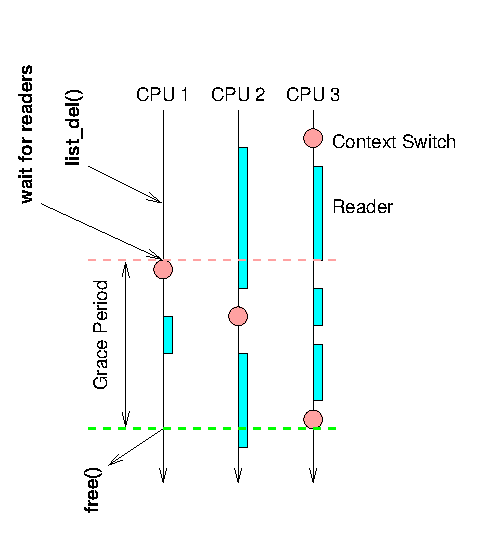
\includegraphics{defer/QSBRGracePeriod}}
\caption{RCU QSBR: Waiting for Pre-Existing Readers}
\label{fig:defer:RCU QSBR: Waiting for Pre-Existing Readers}
\end{figure}

This approach is termed \emph{quiescent state based reclamation}
(QSBR)~\cite{ThomasEHart2006a}.
A QSBR schematic is shown in
Figure~\ref{fig:defer:RCU QSBR: Waiting for Pre-Existing Readers},
with time advancing from the top of the figure to the bottom.

Although production-quality implementations of this approach can be
quite complex, a toy implementation is exceedingly simple:

\vspace{5pt}
\begin{minipage}[t]{\columnwidth}
\scriptsize
\begin{verbatim}
  1 for_each_online_cpu(cpu)
  2   run_on(cpu);
\end{verbatim}
\end{minipage}
\vspace{5pt}

The \co{for_each_online_cpu()} primitive iterates over all CPUs, and
the \co{run_on()} function causes the current thread to execute on the
specified CPU, which forces the destination CPU to execute a context
switch.
Therefore, once the \co{for_each_online_cpu()} has completed, each CPU
has executed a context switch, which in turn guarantees that
all pre-existing reader threads have completed.

Please note that this approach is \emph{not} production quality.
Correct handling of a number of corner cases and the need for a number
of powerful optimizations mean that production-quality implementations
have significant additional complexity.
In addition, RCU implementations for preemptible environments
require that readers actually do something.
However, this simple non-preemptible approach is conceptually complete,
and forms a good initial basis for understanding the RCU fundamentals
covered in the following section.

% defer/rcufundamental.tex

\subsection{RCU Fundamentals}
\label{sec:defer:RCU Fundamentals}
\OriginallyPublished{Section}{sec:defer:RCU Fundamentals}{RCU Fundamentals}{Linux Weekly News}{PaulEMcKenney2007WhatIsRCUFundamentally}

Authors: Paul E. McKenney and Jonathan Walpole

Read-copy update (RCU) is a synchronization mechanism that was added to
the Linux kernel in October of 2002.
RCU achieves scalability
improvements by allowing reads to occur concurrently with updates.
In contrast with conventional locking primitives that ensure mutual exclusion
among concurrent threads regardless of whether they be readers or
updaters, or with reader-writer locks that allow concurrent reads but not in
the presence of updates, RCU supports concurrency between a single
updater and multiple readers.
RCU ensures that reads are coherent by
maintaining multiple versions of objects and ensuring that they are not
freed up until all pre-existing read-side critical sections complete.
RCU defines and uses efficient and scalable mechanisms for publishing
and reading new versions of an object, and also for deferring the collection
of old versions.
These mechanisms distribute the work among read and
update paths in such a way as to make read paths extremely fast. In some
cases (non-preemptible kernels), RCU's read-side primitives have zero
overhead.

\QuickQuiz{}
	But doesn't Section~\ref{sec:defer:Sequence Locks}'s seqlock
	also permit readers and updaters to get work done concurrently?
\QuickQuizAnswer{
	Yes and no.
	Although seqlock readers can run concurrently with
	seqlock writers, whenever this happens, the {\tt read\_seqretry()}
	primitive will force the reader to retry.
	This means that any work done by a seqlock reader running concurrently
	with a seqlock updater will be discarded and redone.
	So seqlock readers can \emph{run} concurrently with updaters,
	but they cannot actually get any work done in this case.

	In contrast, RCU readers can perform useful work even in presence
	of concurrent RCU updaters.
} \QuickQuizEnd

This leads to the question ``what exactly is RCU?'', and perhaps also
to the question ``how can RCU \emph{possibly} work?'' (or, not
infrequently, the assertion that RCU cannot possibly work).
This document addresses these questions from a fundamental viewpoint;
later installments look at them from usage and from API viewpoints.
This last installment also includes a list of references.

RCU is made up of three fundamental mechanisms, the first being
used for insertion, the second being used for deletion, and the third
being used to allow readers to tolerate concurrent insertions and deletions.
Section~\ref{sec:defer:Publish-Subscribe Mechanism}
describes the publish-subscribe mechanism used for insertion,
Section~\ref{sec:defer:Wait For Pre-Existing RCU Readers to Complete}
describes how waiting for pre-existing RCU readers enabled deletion,
and
Section~\ref{sec:defer:Maintain Multiple Versions of Recently Updated Objects}
discusses how maintaining multiple versions of recently updated objects
permits concurrent insertions and deletions.
Finally,
Section~\ref{sec:defer:Summary of RCU Fundamentals}
summarizes RCU fundamentals.

\subsubsection{Publish-Subscribe Mechanism}
\label{sec:defer:Publish-Subscribe Mechanism}

\begin{figure}[tbp]
{ \scriptsize
\begin{verbatim}
  1 struct foo {
  2   int a;
  3   int b;
  4   int c;
  5 };
  6 struct foo *gp = NULL;
  7
  8 /* . . . */
  9
 10 p = kmalloc(sizeof(*p), GFP_KERNEL);
 11 p->a = 1;
 12 p->b = 2;
 13 p->c = 3;
 14 gp = p;
\end{verbatim}
}
\caption{Data Structure Publication (Unsafe)}
\label{fig:defer:Data Structure Publication (Unsafe)}
\end{figure}

One key attribute of RCU is the ability to safely scan data, even
though that data is being modified concurrently.
To provide this ability for concurrent insertion,
RCU uses what can be thought of as a publish-subscribe mechanism.
For example, consider an initially \co{NULL} global pointer
\co{gp} that is to be modified to point to a newly allocated
and initialized data structure.
The code fragment shown in
Figure~\ref{fig:defer:Data Structure Publication (Unsafe)}
(with the addition of appropriate locking)
might be used for this purpose.

Unfortunately, there is nothing forcing the compiler and CPU to execute
the last four assignment statements in order.
If the assignment to \co{gp} happens before the initialization
of \co{p} fields, then concurrent readers could see the
uninitialized values.
Memory barriers are required to keep things ordered, but memory barriers
are notoriously difficult to use.
We therefore encapsulate them into a primitive
\co{rcu_assign_pointer()} that has publication semantics.
The last four lines would then be as follows:

\vspace{5pt}
\begin{minipage}[t]{\columnwidth}
\scriptsize
\begin{verbatim}
  1 p->a = 1;
  2 p->b = 2;
  3 p->c = 3;
  4 rcu_assign_pointer(gp, p);
\end{verbatim}
\end{minipage}
\vspace{5pt}

The \co{rcu_assign_pointer()}
would \emph{publish} the new structure, forcing both the compiler
and the CPU to execute the assignment to \co{gp} \emph{after}
the assignments to the fields referenced by \co{p}.

However, it is not sufficient to only enforce ordering at the
updater, as the reader must enforce proper ordering as well.
Consider for example the following code fragment:

\vspace{5pt}
\begin{minipage}[t]{\columnwidth}
\scriptsize
\begin{verbatim}
  1 p = gp;
  2 if (p != NULL) {
  3   do_something_with(p->a, p->b, p->c);
  4 }
\end{verbatim}
\end{minipage}
\vspace{5pt}

Although this code fragment might well seem immune to misordering,
unfortunately, the
DEC Alpha CPU~\cite{PaulMcKenney2005i,PaulMcKenney2005j}
and value-speculation compiler optimizations can, believe it or not,
cause the values of \co{p->a}, \co{p->b}, and
\co{p->c} to be fetched before the value of \co{p}.
This is perhaps easiest to see in the case of value-speculation
compiler optimizations, where the compiler guesses the value
of \co{p} fetches \co{p->a}, \co{p->b}, and
\co{p->c} then fetches the actual value of \co{p}
in order to check whether its guess was correct.
This sort of optimization is quite aggressive, perhaps insanely so,
but does actually occur in the context of profile-driven optimization.

Clearly, we need to prevent this sort of skullduggery on the
part of both the compiler and the CPU.
The \co{rcu_dereference()} primitive uses
whatever memory-barrier instructions and compiler
directives are required for this purpose:

\vspace{5pt}
\begin{minipage}[t]{\columnwidth}
\scriptsize
\begin{verbatim}
  1 rcu_read_lock();
  2 p = rcu_dereference(gp);
  3 if (p != NULL) {
  4   do_something_with(p->a, p->b, p->c);
  5 }
  6 rcu_read_unlock();
\end{verbatim}
\end{minipage}
\vspace{5pt}

The \co{rcu_dereference()} primitive can thus be thought of
as \emph{subscribing} to a given value of the specified pointer,
guaranteeing that subsequent dereference operations will see any
initialization that occurred before the corresponding
\co{rcu_assign_pointer()} operation that published that pointer.
The \co{rcu_read_lock()} and \co{rcu_read_unlock()}
calls are absolutely required: they define the extent of the
RCU read-side critical section.
Their purpose is explained in
Section~\ref{sec:defer:Wait For Pre-Existing RCU Readers to Complete},
however, they never spin or block, nor do they prevent the
\co{list_add_rcu()} from executing concurrently.
In fact, in non-\co{CONFIG_PREEMPT} kernels, they generate
absolutely no code.

\begin{figure}[tb]
\begin{center}
\resizebox{3in}{!}{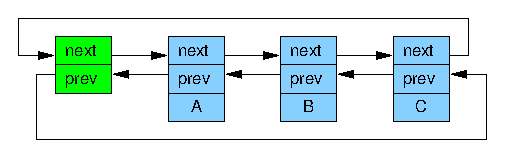
\includegraphics{defer/Linux_list}}
\end{center}
\caption{Linux Circular Linked List}
\label{fig:defer:Linux Circular Linked List}
\end{figure}

\begin{figure}[tb]
\begin{center}
\resizebox{3in}{!}{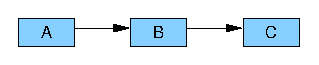
\includegraphics{defer/Linux_list_abbr}}
\end{center}
\caption{Linux Linked List Abbreviated}
\label{fig:defer:Linux Linked List Abbreviated}
\end{figure}

Although \co{rcu_assign_pointer()} and
\co{rcu_dereference()} can in theory be used to construct any
conceivable RCU-protected data structure, in practice it is often better
to use higher-level constructs.
Therefore, the \co{rcu_assign_pointer()} and
\co{rcu_dereference()}
primitives have been embedded in special RCU variants of Linux's
list-manipulation API.
Linux has two variants of doubly linked list, the circular
{\tt struct list\_head} and the linear
{\tt struct hlist\_head}/{\tt struct hlist\_node} pair.
The former is laid out as shown in
Figure~\ref{fig:defer:Linux Circular Linked List},
where the green boxes represent
the list header and the blue boxes represent the elements in the
list.
This notation is cumbersome, and will therefore be abbreviated as shown in
Figure~\ref{fig:defer:Linux Linked List Abbreviated}.

\begin{figure}[tbp]
{ \scriptsize
\begin{verbatim}
  1 struct foo {
  2   struct list_head *list;
  3   int a;
  4   int b;
  5   int c;
  6 };
  7 LIST_HEAD(head);
  8
  9 /* . . . */
 10
 11 p = kmalloc(sizeof(*p), GFP_KERNEL);
 12 p->a = 1;
 13 p->b = 2;
 14 p->c = 3;
 15 list_add_rcu(&p->list, &head);
\end{verbatim}
}
\caption{RCU Data Structure Publication}
\label{fig:defer:RCU Data Structure Publication}
\end{figure}

Adapting the pointer-publish example for the linked list results in
the code shown in
Figure~\ref{fig:defer:RCU Data Structure Publication}.

Line~15 must be protected by some synchronization mechanism (most
commonly some sort of lock) to prevent multiple \co{list_add()}
instances from executing concurrently.
However, such synchronization does not prevent this \co{list_add()}
instance from executing concurrently with RCU readers.

Subscribing to an RCU-protected list is straightforward:

\vspace{5pt}
\begin{minipage}[t]{\columnwidth}
\scriptsize
\begin{verbatim}
  1 rcu_read_lock();
  2 list_for_each_entry_rcu(p, head, list) {
  3   do_something_with(p->a, p->b, p->c);
  4 }
  5 rcu_read_unlock();
\end{verbatim}
\end{minipage}
\vspace{5pt}

The \co{list_add_rcu()} primitive publishes
an entry into the specified list, guaranteeing that the corresponding
\co{list_for_each_entry_rcu()} invocation will properly
subscribe to this same entry.

\QuickQuiz{}
	What prevents the {\tt list\_for\_each\_entry\_rcu()} from
	getting a segfault if it happens to execute at exactly the same
	time as the {\tt list\_add\_rcu()}?
\QuickQuizAnswer{
	On all systems running Linux, loads from and stores
	to pointers are atomic, that is, if a store to a pointer occurs at
	the same time as a load from that same pointer, the load will return
	either the initial value or the value stored, never some bitwise
	mashup of the two.
	In addition, the {\tt list\_for\_each\_entry\_rcu()} always proceeds
	forward through the list, never looking back.
	Therefore, the {\tt list\_for\_each\_entry\_rcu()} will either see
	the element being added by {\tt list\_add\_rcu()} or it will not,
	but either way, it will see a valid well-formed list.
} \QuickQuizEnd

\begin{figure}[tb]
\begin{center}
\resizebox{3in}{!}{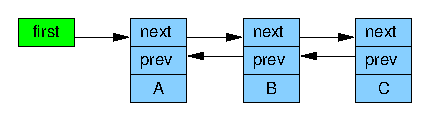
\includegraphics{defer/Linux_hlist}}
\end{center}
\caption{Linux Linear Linked List}
\label{fig:defer:Linux Linear Linked List}
\end{figure}

Linux's other doubly linked list, the hlist,
is a linear list, which means that
it needs only one pointer for the header rather than the two
required for the circular list, as shown in
Figure~\ref{fig:defer:Linux Linear Linked List}.
Thus, use of hlist can halve the memory consumption for the hash-bucket
arrays of large hash tables.
As before, this notation is cumbersome, so hlists will be abbreviated
in the same way lists are, as shown in
Figure~\ref{fig:defer:Linux Linked List Abbreviated}.

\begin{figure}[tbp]
{ \scriptsize
\begin{verbatim}
  1 struct foo {
  2   struct hlist_node *list;
  3   int a;
  4   int b;
  5   int c;
  6 };
  7 HLIST_HEAD(head);
  8
  9 /* . . . */
 10
 11 p = kmalloc(sizeof(*p), GFP_KERNEL);
 12 p->a = 1;
 13 p->b = 2;
 14 p->c = 3;
 15 hlist_add_head_rcu(&p->list, &head);
\end{verbatim}
}
\caption{RCU {\tt hlist} Publication}
\label{fig:defer:RCU hlist Publication}
\end{figure}

Publishing a new element to an RCU-protected hlist is quite similar
to doing so for the circular list,
as shown in Figure~\ref{fig:defer:RCU hlist Publication}.

As before, line~15 must be protected by some sort of synchronization
mechanism, for example, a lock.

Subscribing to an RCU-protected hlist is also similar to the
circular list:

\vspace{5pt}
\begin{minipage}[t]{\columnwidth}
\scriptsize
\begin{verbatim}
  1 rcu_read_lock();
  2 hlist_for_each_entry_rcu(p, q, head, list) {
  3   do_something_with(p->a, p->b, p->c);
  4 }
  5 rcu_read_unlock();
\end{verbatim}
\end{minipage}
\vspace{5pt}

\QuickQuiz{}
	Why do we need to pass two pointers into
	{\tt hlist\_for\_each\_entry\_rcu()}
	when only one is needed for {\tt list\_for\_each\_entry\_rcu()}?
\QuickQuizAnswer{
	Because in an hlist it is necessary to check for
	NULL rather than for encountering the head.
	(Try coding up a single-pointer {\tt hlist\_for\_each\_entry\_rcu()}
	If you come up with a nice solution, it would be a very good thing!)
} \QuickQuizEnd

\begin{table*}[tb]
\begin{center}
\scriptsize
\begin{tabular}{l||l|l|l}
Category  & Publish	& Retract	& Subscribe \\
\hline
\hline
Pointers  & \co{rcu_assign_pointer()}
			& \co{rcu_assign_pointer(..., NULL)}~~
					& \co{rcu_dereference()} \\
\hline
Lists     & \parbox{1.5in}{
		\co{list_add_rcu()} \\
		\co{list_add_tail_rcu()} \\
		\co{list_replace_rcu()} }
			& \co{list_del_rcu()}
					& \co{list_for_each_entry_rcu()}~~~ \\
\hline
Hlists    & \parbox{1.5in}{
		\co{hlist_add_after_rcu()} \\
		\co{hlist_add_before_rcu()}  \\
		\co{hlist_add_head_rcu()} \\
		\co{hlist_replace_rcu()} }
			& \co{hlist_del_rcu()}
					& \co{hlist_for_each_entry_rcu()}~~~~~
\end{tabular}
\end{center}
\caption{RCU Publish and Subscribe Primitives}
\label{tab:defer:RCU Publish and Subscribe Primitives}
\end{table*}

The set of RCU publish and subscribe primitives are shown in
Table~\ref{tab:defer:RCU Publish and Subscribe Primitives},
along with additional primitives to ``unpublish'', or retract.

Note that the \co{list_replace_rcu()}, \co{list_del_rcu()},
\co{hlist_replace_rcu()}, and \co{hlist_del_rcu()}
APIs add a complication.
When is it safe to free up the data element that was replaced or
removed?
In particular, how can we possibly know when all the readers
have released their references to that data element?

These questions are addressed in the following section.

\subsubsection{Wait For Pre-Existing RCU Readers to Complete}
\label{sec:defer:Wait For Pre-Existing RCU Readers to Complete}

In its most basic form, RCU is a way of waiting for things to finish.
Of course, there are a great many other ways of waiting for things to
finish, including reference counts, reader-writer locks, events, and so on.
The great advantage of RCU is that it can wait for each of
(say) 20,000 different things without having to explicitly
track each and every one of them, and without having to worry about
the performance degradation, scalability limitations, complex deadlock
scenarios, and memory-leak hazards that are inherent in schemes
using explicit tracking.

In RCU's case, the things waited on are called
``RCU read-side critical sections''.
An RCU read-side critical section starts with an
\co{rcu_read_lock()} primitive, and ends with a corresponding
\co{rcu_read_unlock()} primitive.
RCU read-side critical sections can be nested, and may contain pretty
much any code, as long as that code does not explicitly block or sleep
(although a special form of RCU called SRCU~\cite{PaulEMcKenney2006c}
does permit general sleeping in SRCU read-side critical sections).
If you abide by these conventions, you can use RCU to wait for \emph{any}
desired piece of code to complete.

RCU accomplishes this feat by indirectly determining when these
other things have finished~\cite{PaulEMcKenney2007whatisRCU,
PaulEMcKenney2007PreemptibleRCU}, as is described in detail in
Appendix~\ref{app:rcuimpl:Read-Copy Update Implementations}.

\begin{figure}[tb]
\begin{center}
\resizebox{3in}{!}{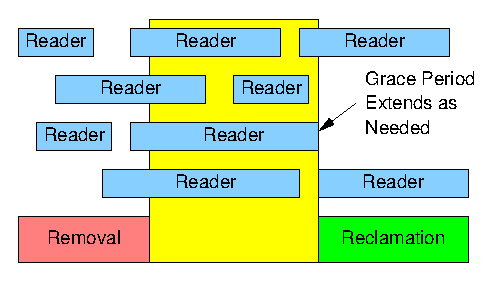
\includegraphics{defer/GracePeriodGood}}
\end{center}
\caption{Readers and RCU Grace Period}
\label{fig:defer:Readers and RCU Grace Period}
\end{figure}

In particular, as shown in
Figure~\ref{fig:defer:Readers and RCU Grace Period},
RCU is a way of
waiting for pre-existing RCU read-side critical sections to completely
finish, including memory operations executed by those critical sections.
However, note that RCU read-side critical sections
that begin after the beginning
of a given grace period can and will extend beyond the end of that grace
period.

The following pseudocode shows the basic form of algorithms that use
RCU to wait for readers:

\begin{enumerate}
\item	Make a change, for example, replace an element in a linked list.
\item	Wait for all pre-existing RCU read-side critical sections to
	completely finish (for example, by using the
	\co{synchronize_rcu()} primitive).
	The key observation here is that subsequent RCU read-side critical
	sections have no way to gain a reference to the newly removed
	element.
\item	Clean up, for example, free the element that was replaced above.
\end{enumerate}

\begin{figure}[tbp]
{ \scriptsize
\begin{verbatim}
  1 struct foo {
  2   struct list_head *list;
  3   int a;
  4   int b;
  5   int c;
  6 };
  7 LIST_HEAD(head);
  8
  9 /* . . . */
 10
 11 p = search(head, key);
 12 if (p == NULL) {
 13   /* Take appropriate action, unlock, & return. */
 14 }
 15 q = kmalloc(sizeof(*p), GFP_KERNEL);
 16 *q = *p;
 17 q->b = 2;
 18 q->c = 3;
 19 list_replace_rcu(&p->list, &q->list);
 20 synchronize_rcu();
 21 kfree(p);
\end{verbatim}
}
\caption{Canonical RCU Replacement Example}
\label{fig:defer:Canonical RCU Replacement Example}
\end{figure}

The code fragment shown in
Figure~\ref{fig:defer:Canonical RCU Replacement Example},
adapted from those in Section~\ref{sec:defer:Publish-Subscribe Mechanism},
demonstrates this process, with field \co{a} being the search key.

Lines~19, 20, and 21 implement the three steps called out above.
Lines~16-19 gives RCU (``read-copy update'') its name: while permitting
concurrent \emph{reads}, line~16 \emph{copies} and lines~17-19
do an \emph{update}.

As discussed in Section~\ref{sec:defer:Introduction to RCU},
the \co{synchronize_rcu()} primitive can be quite simple
(see Section~\ref{sec:defer:``Toy'' RCU Implementations}
for additional ``toy'' RCU implementations).
However, production-quality implementations must deal with
difficult corner cases and also incorporate
powerful optimizations, both of which result in significant complexity.
Although it is good to know that there is a simple conceptual
implementation of \co{synchronize_rcu()}, other questions remain.
For example, what exactly do RCU
readers see when traversing a concurrently updated list?
This question is addressed in the following section.

\subsubsection{Maintain Multiple Versions of Recently Updated Objects}
\label{sec:defer:Maintain Multiple Versions of Recently Updated Objects}

This section demonstrates how RCU maintains multiple versions of
lists to accommodate synchronization-free readers.
Two examples are presented showing how an element
that might be referenced by a given reader must remain intact
while that reader remains in its RCU read-side critical section.
The first example demonstrates deletion of a list element,
and the second example demonstrates replacement of an element.

\paragraph{Example 1: Maintaining Multiple Versions During Deletion}
\label{sec:defer:Example 1: Maintaining Multiple Versions During Deletion}

We can now revisit the deletion example from
Section~\ref{sec:defer:Introduction to RCU},
but now with the benefit of a firm understanding of the fundamental
concepts underlying RCU.
To begin this new version of the deletion example,
we will modify lines~11-21 in
Figure~\ref{fig:defer:Canonical RCU Replacement Example}
to read as follows:

\vspace{5pt}
\begin{minipage}[t]{\columnwidth}
\scriptsize
\begin{verbatim}
  1 p = search(head, key);
  2 if (p != NULL) {
  3   list_del_rcu(&p->list);
  4   synchronize_rcu();
  5   kfree(p);
  6 }
\end{verbatim}
\end{minipage}
\vspace{5pt}

\begin{figure}[tb]
\begin{center}
\resizebox{3in}{!}{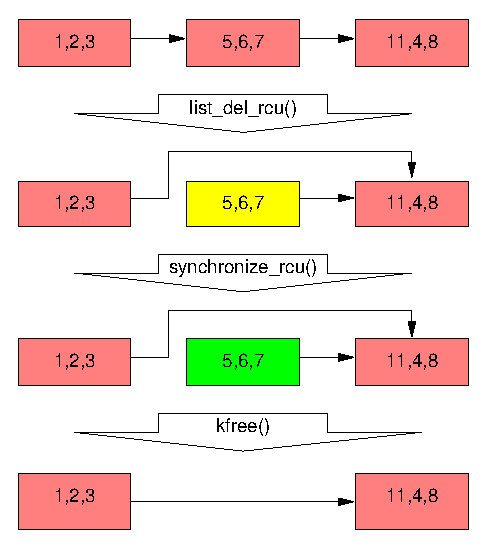
\includegraphics{defer/RCUDeletion}}
\end{center}
\caption{RCU Deletion From Linked List}
\label{fig:defer:RCU Deletion From Linked List}
\end{figure}

This code will update the list as shown in
Figure~\ref{fig:defer:RCU Deletion From Linked List}.
The triples in each element represent the values of fields \co{a},
\co{b}, and \co{c}, respectively.
The red-shaded elements
indicate that RCU readers might be holding references to them.
Please note that
we have omitted the backwards pointers and the link from the tail
of the list to the head for clarity.

After the \co{list_del_rcu()} on
line~3 has completed, the \co{5,6,7}~element
has been removed from the list, as shown in the second row of
Figure~\ref{fig:defer:RCU Deletion From Linked List}.
Since readers do not synchronize directly with updaters,
readers might be concurrently scanning this list.
These concurrent readers might or might not see the newly removed element,
depending on timing.
However, readers that were delayed (e.g., due to interrupts, ECC memory
errors, or, in \co{CONFIG_PREEMPT_RT} kernels, preemption)
just after fetching a pointer to the newly removed element might
see the old version of the list for quite some time after the
removal.
Therefore, we now have two versions of the list, one with element
\co{5,6,7} and one without.
The \co{5,6,7}~element is
shaded yellow, indicating
that old readers might still be referencing it, but that new
readers cannot obtain a reference to it.

Please note that readers are not permitted to maintain references to
element~\co{5,6,7} after exiting from their RCU read-side
critical sections.
Therefore,
once the \co{synchronize_rcu()} on
line~4 completes, so that all pre-existing readers are
guaranteed to have completed,
there can be no more readers referencing this
element, as indicated by its green shading on the third row of
Figure~\ref{fig:defer:RCU Deletion From Linked List}.
We are thus back to a single version of the list.

At this point, the \co{5,6,7}~element may safely be
freed, as shown on the final row of
Figure~\ref{fig:defer:RCU Deletion From Linked List}.
At this point, we have completed the deletion of
element~\co{5,6,7}.
The following section covers replacement.

\paragraph{Example 2: Maintaining Multiple Versions During Replacement}
\label{sec:defer:Example 2: Maintaining Multiple Versions During Replacement}

To start the replacement example,
here are the last few lines of the
example shown in
Figure~\ref{fig:defer:Canonical RCU Replacement Example}:

\vspace{5pt}
\begin{minipage}[t]{\columnwidth}
\scriptsize
\begin{verbatim}
  1 q = kmalloc(sizeof(*p), GFP_KERNEL);
  2 *q = *p;
  3 q->b = 2;
  4 q->c = 3;
  5 list_replace_rcu(&p->list, &q->list);
  6 synchronize_rcu();
  7 kfree(p);
\end{verbatim}
\end{minipage}
\vspace{5pt}

\begin{figure}[tbp]
\begin{center}
\resizebox{2.7in}{!}{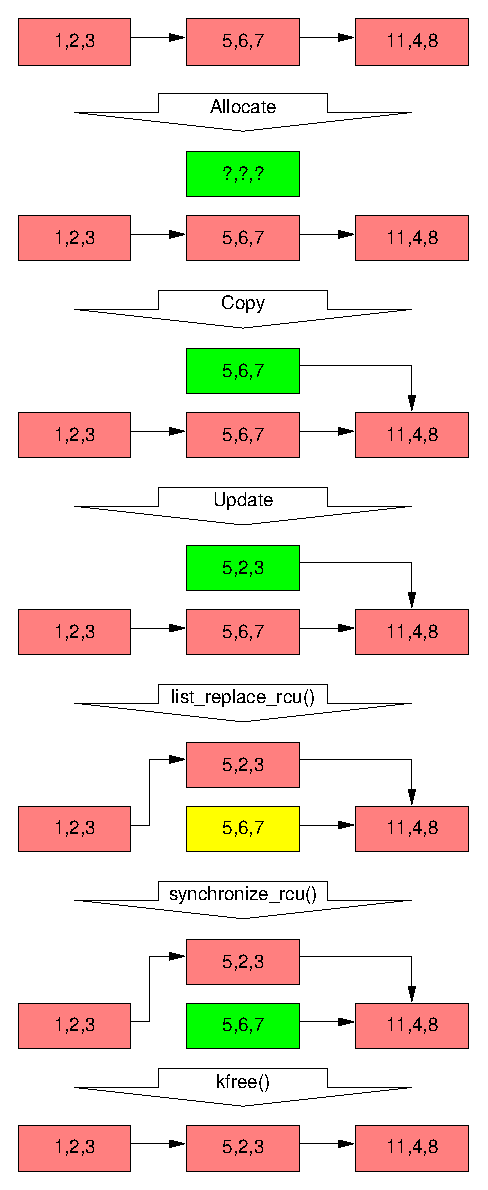
\includegraphics{defer/RCUReplacement}}
\end{center}
\caption{RCU Replacement in Linked List}
\label{fig:defer:RCU Replacement in Linked List}
\end{figure}

The initial state of the list, including the pointer \co{p},
is the same as for the deletion example, as shown on the
first row of
Figure~\ref{fig:defer:RCU Replacement in Linked List}.

As before,
the triples in each element represent the values of fields \co{a},
\co{b}, and \co{c}, respectively.
The red-shaded elements might be referenced by readers,
and because readers do not synchronize directly with updaters,
readers might run concurrently with this entire replacement process.
Please note that
we again omit the backwards pointers and the link from the tail
of the list to the head for clarity.

The following text describes how to replace the \co{5,6,7} element
with \co{5,2,3} in such a way that any given reader sees one of these
two values.

Line~1 \co{kmalloc()}s a replacement element, as follows,
resulting in the state as shown in the second row of
Figure~\ref{fig:defer:RCU Replacement in Linked List}.
At this point, no reader can hold a reference to the newly allocated
element (as indicated by its green shading), and it is uninitialized
(as indicated by the question marks).

Line~2 copies the old element to the new one, resulting in the
state as shown in the third row of
Figure~\ref{fig:defer:RCU Replacement in Linked List}.
The newly allocated element still cannot be referenced by readers, but
it is now initialized.

Line~3 updates \co{q->b} to the value ``2'', and
line~4 updates \co{q->c} to the value ``3'', as shown on the fourth row of
Figure~\ref{fig:defer:RCU Replacement in Linked List}.

Now, line~5 does the replacement, so that the new element is
finally visible to readers, and hence is shaded red, as shown on
the fifth row of
Figure~\ref{fig:defer:RCU Replacement in Linked List}.
At this point, as shown below, we have two versions of the list.
Pre-existing readers might see the \co{5,6,7} element (which is
therefore now shaded yellow), but
new readers will instead see the \co{5,2,3} element.
But any given reader is guaranteed to see some well-defined list.

After the \co{synchronize_rcu()} on line~6 returns,
a grace period will have elapsed, and so all reads that started before the
\co{list_replace_rcu()} will have completed.
In particular, any readers that might have been holding references
to the \co{5,6,7} element are guaranteed to have exited
their RCU read-side critical sections, and are thus prohibited from
continuing to hold a reference.
Therefore, there can no longer be any readers holding references
to the old element, as indicated its green shading in the sixth row of
Figure~\ref{fig:defer:RCU Replacement in Linked List}.
As far as the readers are concerned, we are back to having a single version
of the list, but with the new element in place of the old.

After the \co{kfree()} on line 7 completes, the list will
appear as shown on the final row of
Figure~\ref{fig:defer:RCU Replacement in Linked List}.

Despite the fact that RCU was named after the replacement case,
the vast majority of RCU usage within the Linux kernel relies on
the simple deletion case shown in
Section~\ref{sec:defer:Maintain Multiple Versions of Recently Updated Objects}.

\paragraph{Discussion}
\label{sec:defer:Discussion}

These examples assumed that a mutex was held across the entire
update operation, which would mean that there could be at most two
versions of the list active at a given time.

\QuickQuiz{}
	How would you modify the deletion example to permit more than two
	versions of the list to be active?
\QuickQuizAnswer{
	One way of accomplishing this is as shown in
	Figure~\ref{fig:defer:Concurrent RCU Deletion}.

\begin{figure}[htbp]
{ \centering
\begin{verbatim}
  1 spin_lock(&mylock);
  2 p = search(head, key);
  3 if (p == NULL)
  4   spin_unlock(&mylock);
  5 else {
  6   list_del_rcu(&p->list);
  7   spin_unlock(&mylock);
  8   synchronize_rcu();
  9   kfree(p);
 10 }
\end{verbatim}
}
\caption{Concurrent RCU Deletion}
\label{fig:defer:Concurrent RCU Deletion}
\end{figure}

	Note that this means that multiple concurrent deletions might be
	waiting in {\tt synchronize\_rcu()}.
} \QuickQuizEnd

\QuickQuiz{}
	How many RCU versions of a given list can be
	active at any given time?
\QuickQuizAnswer{
	That depends on the synchronization design.
	If a semaphore protecting the update is held across the grace period,
	then there can be at most two versions, the old and the new.

	However, if only the search, the update, and the
	{\tt list\_replace\_rcu()} were protected by a lock, then
	there could be an arbitrary number of versions active, limited only
	by memory and by how many updates could be completed within a
	grace period.
	But please note that data structures that are updated so frequently
	probably are not good candidates for RCU.
	That said, RCU can handle high update rates when necessary.
} \QuickQuizEnd

This sequence of events shows how RCU updates use multiple versions
to safely carry out changes in presence of concurrent readers.
Of course, some algorithms cannot gracefully handle multiple versions.
There are techniques
for adapting such algorithms to RCU~\cite{PaulEdwardMcKenneyPhD},
but these are beyond the scope of this section.

\subsubsection{Summary of RCU Fundamentals}
\label{sec:defer:Summary of RCU Fundamentals}

This section has described the three fundamental components of RCU-based
algorithms:

\begin{enumerate}
\item	a publish-subscribe mechanism for adding new data,

\item	a way of waiting for pre-existing RCU readers to finish, and

\item	a discipline of maintaining multiple versions to permit
	change without harming or unduly delaying concurrent RCU readers.
\end{enumerate}

\QuickQuiz{}
	How can RCU updaters possibly delay RCU readers, given that the
	{\tt rcu\_read\_lock()} and {\tt rcu\_read\_unlock()}
	primitives neither spin nor block?
\QuickQuizAnswer{
	The modifications undertaken by a given RCU updater will cause the
	corresponding CPU to invalidate cache lines containing the data,
	forcing the CPUs running concurrent RCU readers to incur expensive
	cache misses.
	(Can you design an algorithm that changes a data structure
	\emph{without}
	inflicting expensive cache misses on concurrent readers?
	On subsequent readers?)
} \QuickQuizEnd

These three RCU components
allow data to be updated in face of concurrent readers, and
can be combined in different ways to
implement a surprising variety of different types of RCU-based algorithms,
some of which are described in the following section.

% defer/rcuusage.tex

\subsection{RCU Usage}
\label{sec:defer:RCU Usage}

\begin{table}[tb]
\begin{center}
\scriptsize
\begin{tabular}{l|l}
Mechanism RCU Replaces & Section \\
\hline
\hline
Reader-writer locking &
	Section~\ref{sec:defer:RCU is a Reader-Writer Lock Replacement} \\
Restricted reference-counting mechanism &
	Section~\ref{sec:defer:RCU is a Restricted Reference-Counting Mechanism} \\
Bulk reference-counting mechanism &
	Section~\ref{sec:defer:RCU is a Bulk Reference-Counting Mechanism} \\
Poor man's garbage collector &
	Section~\ref{sec:defer:RCU is a Poor Man's Garbage Collector} \\
Existence Guarantees &
	Section~\ref{sec:defer:RCU is a Way of Providing Existence Guarantees} \\
Type-Safe Memory &
	Section~\ref{sec:deferRCU is a Way of Providing Type-Safe Memory} \\
Wait for things to finish &
	Section~\ref{sec:deferRCU is a Way of Waiting for Things to Finish} \\
\end{tabular}
\end{center}
\caption{RCU Usage}
\label{tab:defer:RCU Usage}
\end{table}

This section answers the question "what is RCU?" from the viewpoint
of the uses to which RCU can be put.
Because RCU is most frequently used to replace some existing mechanism,
we look at it primarily in terms of its relationship to such mechanisms,
as listed in Table~\ref{tab:defer:RCU Usage}.
Following the sections listed in this table,
Section~\ref{sec:defer:RCU Usage Summary} provides a summary.

\subsubsection{RCU is a Reader-Writer Lock Replacement}
\label{sec:defer:RCU is a Reader-Writer Lock Replacement}

Perhaps the most common use of RCU within the Linux kernel is as
a replacement for reader-writer locking in read-intensive situations.
Nevertheless, this use of RCU was not immediately apparent to me
at the outset, in fact, I chose to implement something similar to
\url{brlock} before implementing a general-purpose RCU implementation
back in the early 1990s.
Each and every one of the uses I envisioned for the proto-brlock
primitive was instead implemented using RCU.
In fact, it was more than
three years before the proto-\url{brlock} primitive saw its first use.
Boy, did I feel foolish!

The key similarity between RCU and reader-writer locking is that
both have read-side critical sections that can execute in parallel.
In fact, in some cases, it is possible to mechanically substitute RCU API
members for the corresponding reader-writer lock API members.
But first, why bother?

Advantages of RCU include performance,
deadlock immunity, and realtime latency.
There are, of course, limitations to RCU, including the fact that
readers and updaters run concurrently, that low-priority RCU readers
can block high-priority threads waiting for a grace period to elapse,
and that grace-period latencies can extend for many milliseconds.
These advantages and limitations are discussed in the following sections.

\paragraph{Performance}

\begin{figure}[tb]
\begin{center}
\resizebox{3in}{!}{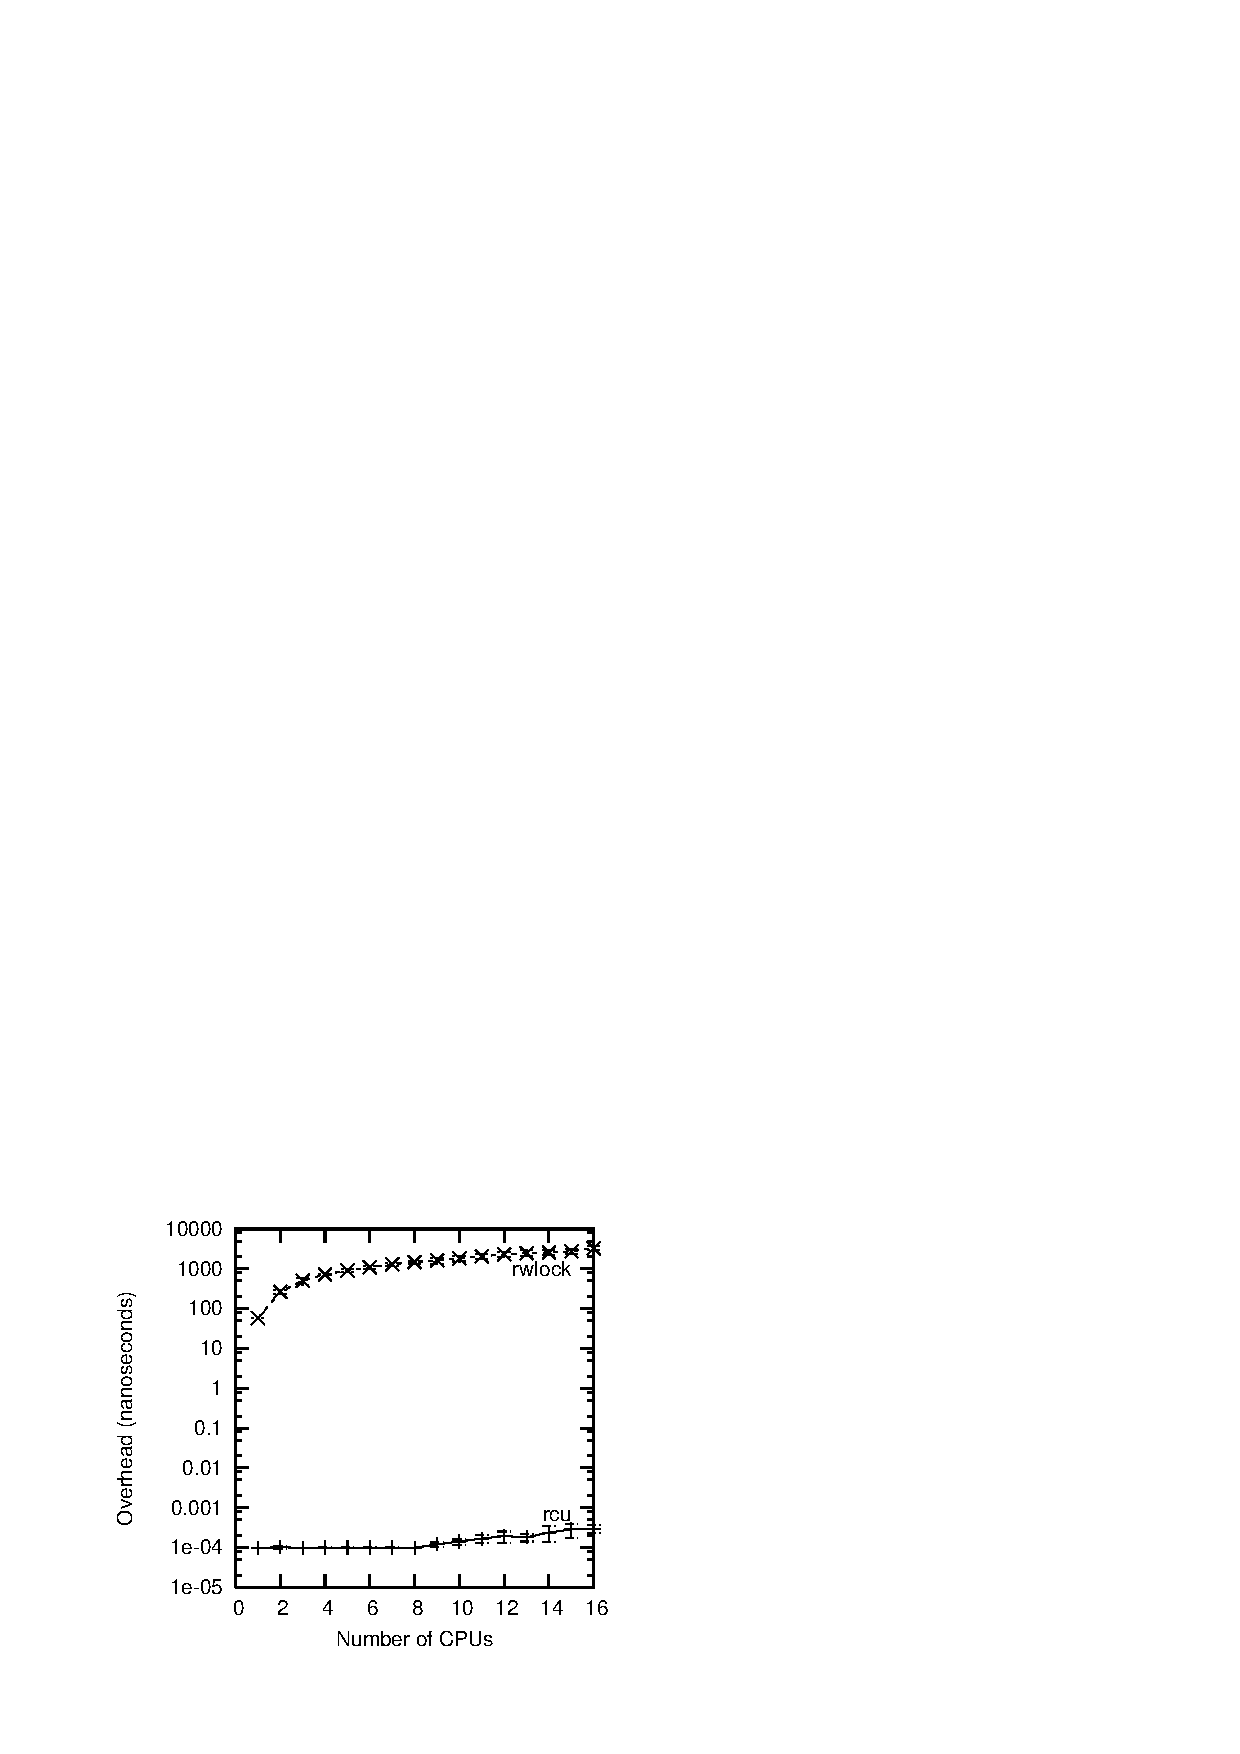
\includegraphics{defer/rwlockRCUperf}}
\end{center}
\caption{Performance Advantage of RCU Over Reader-Writer Locking}
\label{fig:defer:Performance Advantage of RCU Over Reader-Writer Locking}
\end{figure}

The read-side performance advantages of RCU over reader-writer locking
are shown in
Figure~\ref{fig:defer:Performance Advantage of RCU Over Reader-Writer Locking}.

\QuickQuiz{
WTF???
How the heck do you expect me to believe that RCU has a
100-femtosecond overhead when the clock period at 3GHz is more than
300 \emph{picoseconds}?}
\QuickQuizAnswer{
First, consider that the inner loop used to
take this measurement is as follows:

\vspace{5pt}
\begin{minipage}[t]{\columnwidth}
\small
\begin{verbatim}
  1 for (i = 0; i < CSCOUNT_SCALE; i++) {
  2   rcu_read_lock();
  3   rcu_read_unlock();
  4 }
\end{verbatim}
\end{minipage}
\vspace{5pt}

Next, consider the effective definitions of \url{rcu_read_lock()}
and \url{rcu_read_unlock()}:

\vspace{5pt}
\begin{minipage}[t]{\columnwidth}
\small
\begin{verbatim}
  1 #define rcu_read_lock()   do { } while (0)
  2 #define rcu_read_unlock() do { } while (0)
\end{verbatim}
\end{minipage}
\vspace{5pt}

Consider also that the compiler does simple optimizations,
allowing it to replace the loop with:

\vspace{5pt}
\begin{minipage}[t]{\columnwidth}
\small
\begin{verbatim}
i = CSCOUNT_SCALE;
\end{verbatim}
\end{minipage}
\vspace{5pt}

So the "measurement" of 100 femtoseconds is simply the fixed
overhead of the timing measurements divided by the number of
passes through the inner loop containing the calls
to \url{rcu_read_lock()} and \url{rcu_read_unlock()}.
And therefore, this measurement really is in error, in fact,
in error by an arbitrary number of orders of magnitude.
As you can see by the definition of \url{rcu_read_lock()}
and \url{rcu_read_unlock()} above, the actual overhead
is precisely zero.

It certainly is not every day that a timing measurement of
100 femtoseconds turns out to be an overestimate!
} \QuickQuizEnd

Note that reader-writer locking is orders of magnitude slower than RCU
on a single CPU, and is almost two \emph{additional} orders of magnitude
slower on 16 CPUs.
In contrast, RCU scales quite well.
In both cases, the error bars span a single standard deviation in either
direction.

\begin{figure}[tb]
\begin{center}
\resizebox{3in}{!}{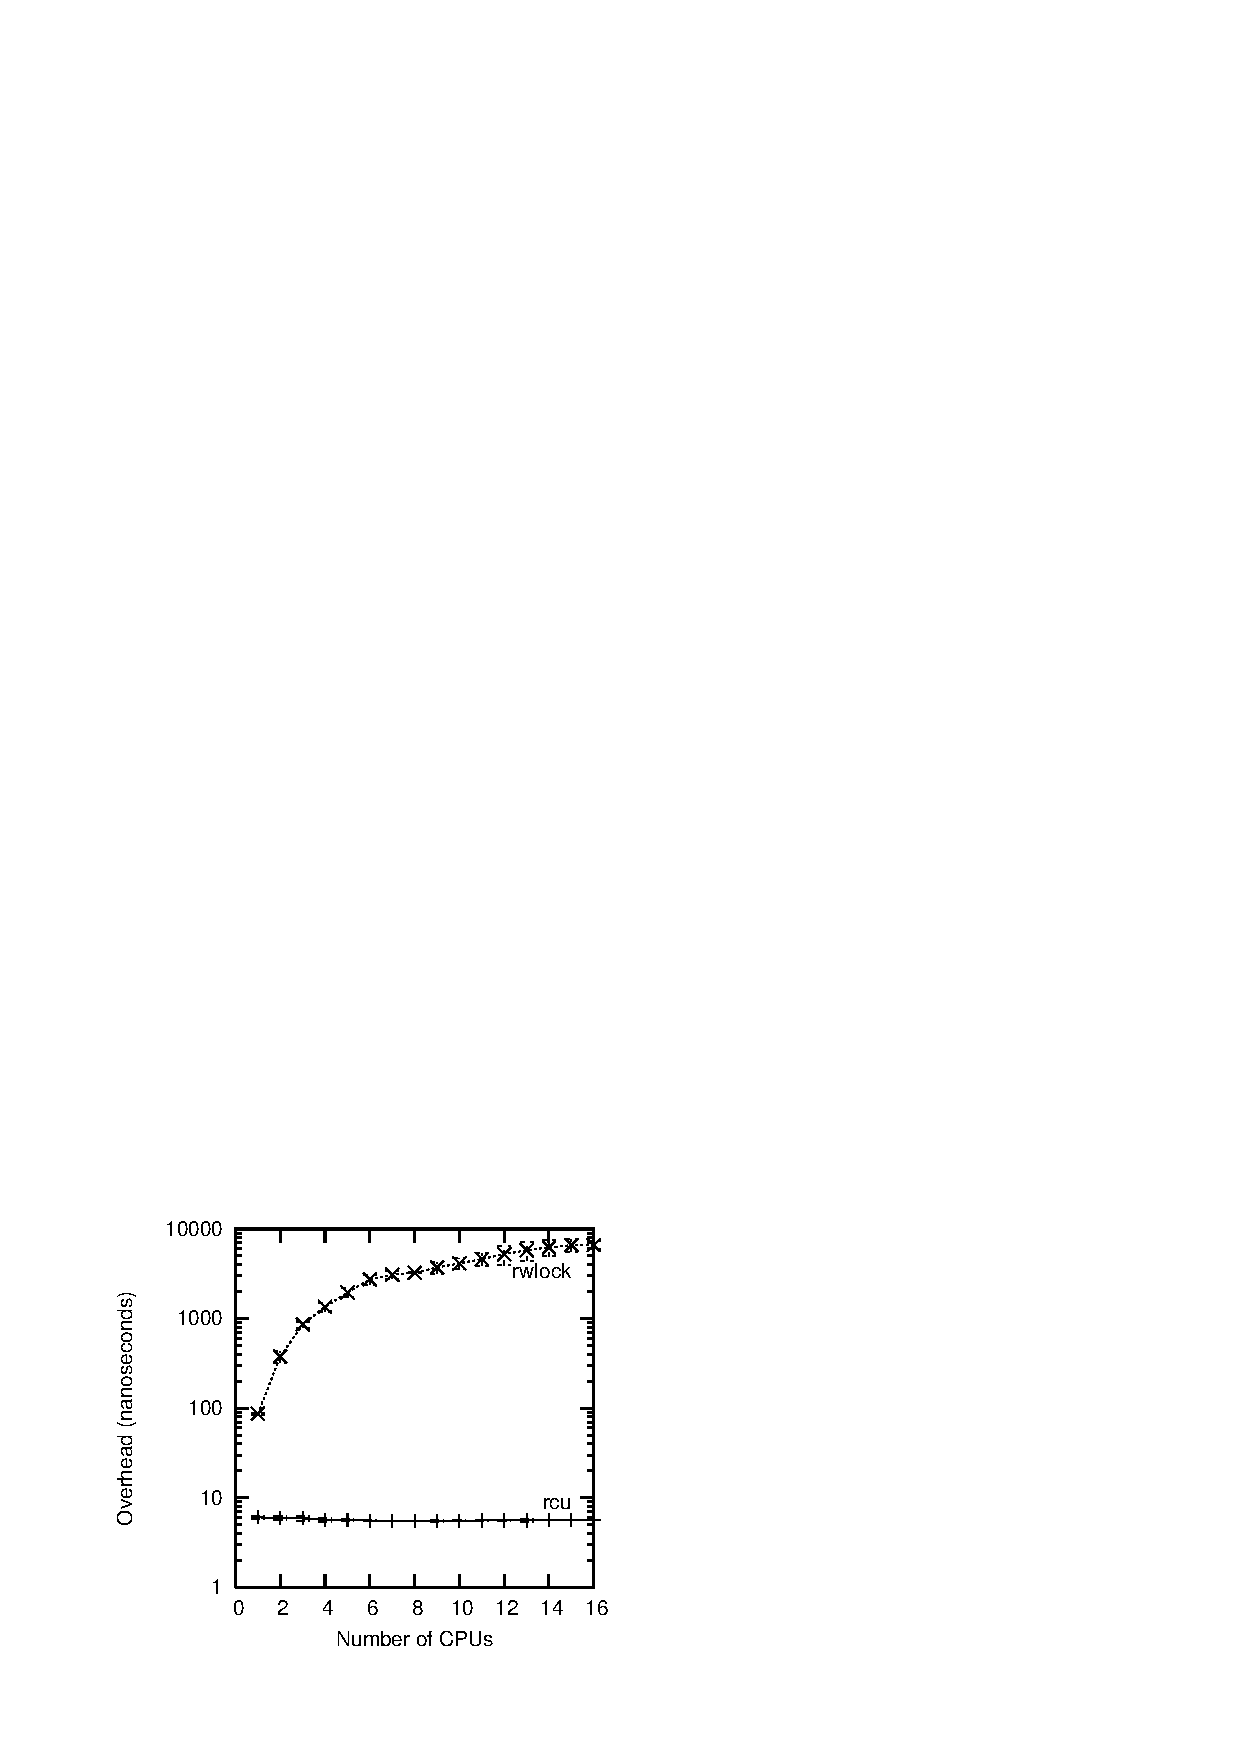
\includegraphics{defer/rwlockRCUperfPREEMPT}}
\end{center}
\caption{Performance Advantage of Preemptable RCU Over Reader-Writer Locking}
\label{fig:defer:Performance Advantage of Preemptable RCU Over Reader-Writer Locking}
\end{figure}

A more moderate view may be obtained from a \url{CONFIG_PREEMPT}
kernel, though RCU still beats reader-writer locking by between one and
three orders of magnitude, as shown in
Figure~\ref{fig:defer:Performance Advantage of Preemptable RCU Over Reader-Writer Locking}.
Note the high variability of reader-writer locking at larger numbers of CPUs.
The error bars span a single standard deviation in either direction.

\begin{figure}[tb]
\begin{center}
\resizebox{3in}{!}{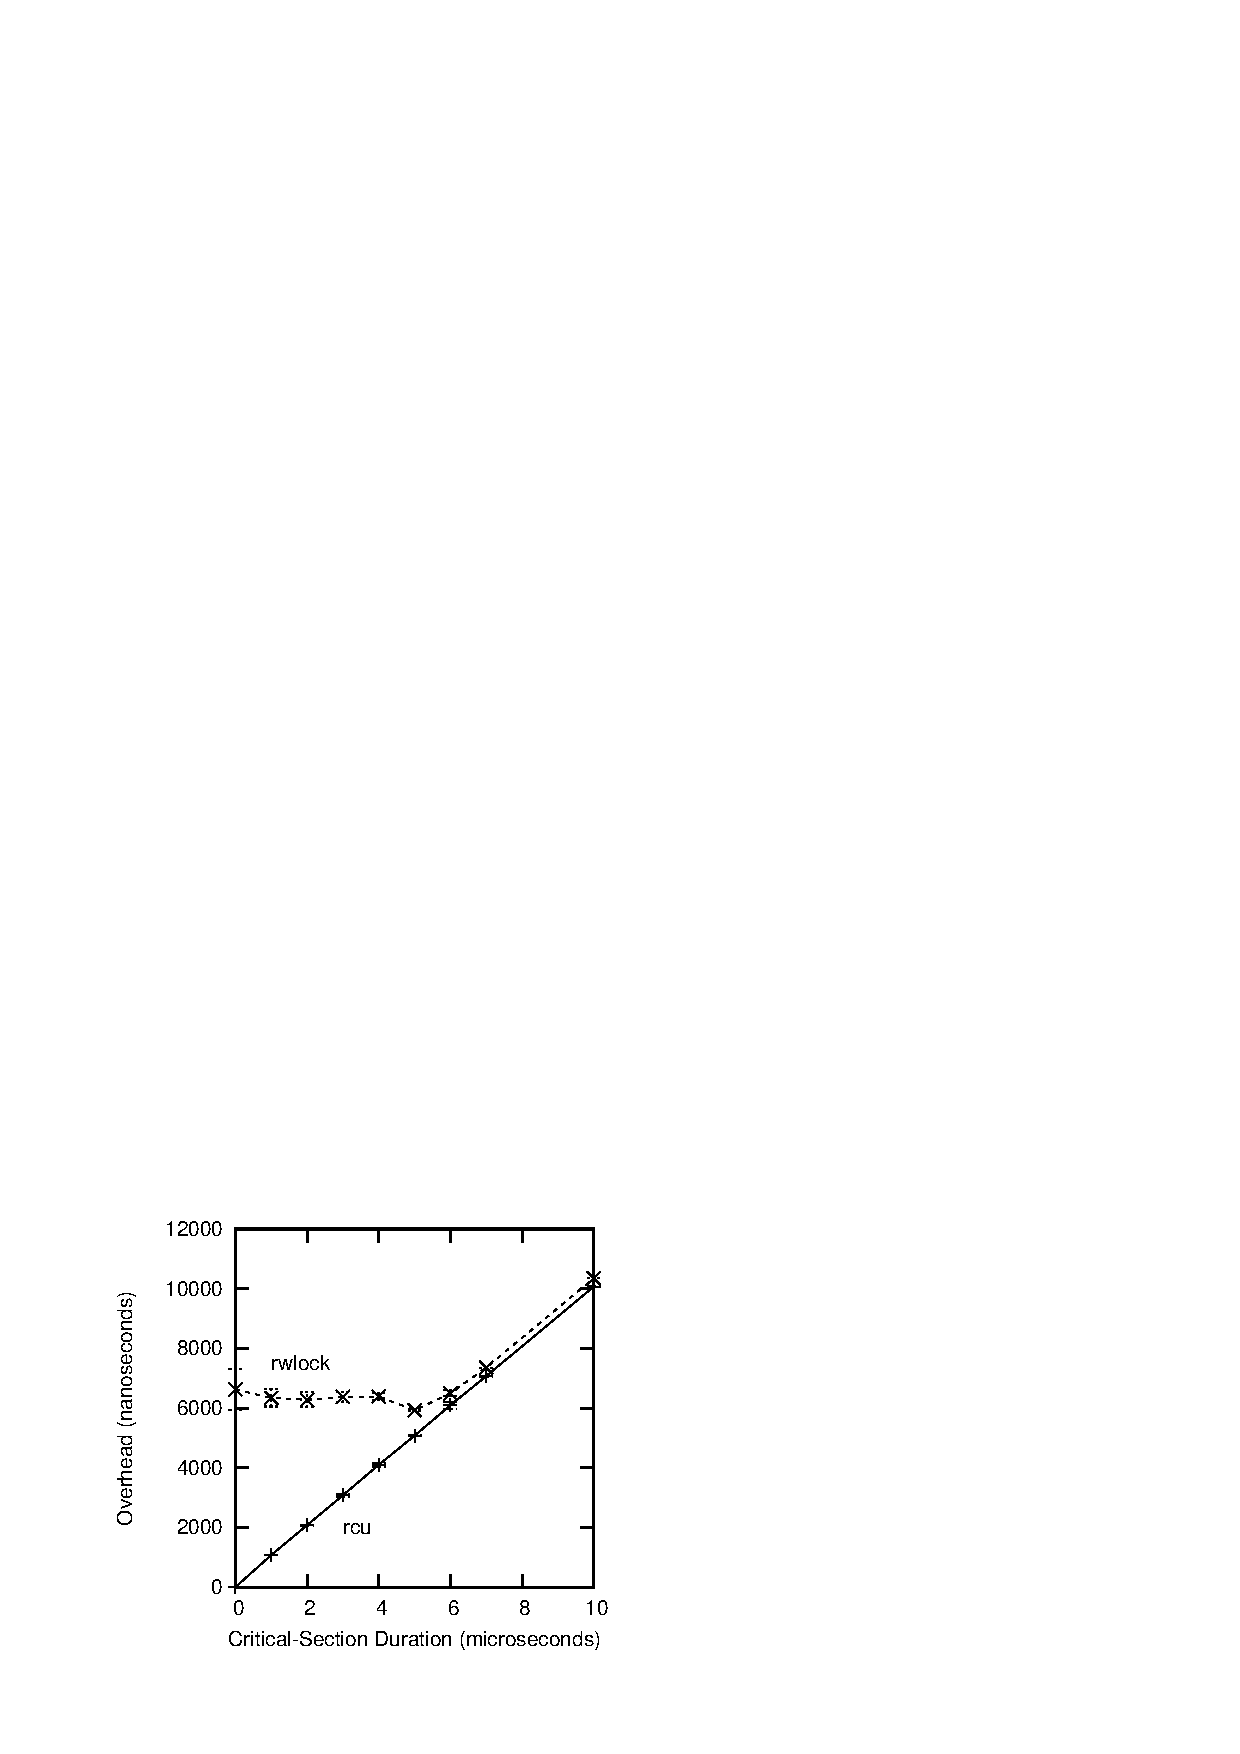
\includegraphics{defer/rwlockRCUperfwtPREEMPT}}
\end{center}
\caption{Comparison of RCU to Reader-Writer Locking as Function of Critical-Section Duration}
\label{fig:defer:Comparison of RCU to Reader-Writer Locking as Function of Critical-Section Duration}
\end{figure}

Of course, the low performance of reader-writer locking in
Figure~\ref{fig:defer:Performance Advantage of Preemptable RCU Over Reader-Writer Locking}
is exaggerated by the unrealistic zero-length critical sections.
The performance advantages of RCU become less significant as the overhead
of the critical section increases, as shown in
Figure~\ref{fig:defer:Comparison of RCU to Reader-Writer Locking as Function of Critical-Section Duration}
for a 16-CPU system,
in which the y-axis represents the sum of the overhead
of the read-side primitives and that of the critical section.

\QuickQuiz{
Why does both the variability and overhead of rwlock decrease as the
critical-section overhead increases?}
\QuickQuizAnswer{
Because the contention on the underlying
\url{rwlock_t} decreases as the critical-section overhead
increases.
However, the rwlock overhead will not quite drop to that on a single
CPU because of cache-thrashing overhead.
} \QuickQuizEnd

However, this observation must be tempered by the fact that
a number of system calls (and thus any RCU read-side critical sections
that they contain) can complete within a few microseconds.

In addition, as is discussed in the next section,
RCU read-side primitives are almost entirely deadlock-immune.


\paragraph{Deadlock Immunity}

Although RCU offers significant performance advantages for
read-mostly workloads, one of the primary reasons for creating
RCU in the first place was in fact its immunity to read-side
deadlocks.
This immunity stems from the fact that
RCU read-side primitives do not block, spin, or even
do backwards branches, so that their execution time is deterministic.
It is therefore impossible for them to participate in a deadlock
cycle.

\QuickQuiz{
Is there an exception to this deadlock immunity, and if so,
what sequence of events could lead to deadlock?}
\QuickQuizAnswer{
One way to cause a deadlock cycle involving
RCU read-side primitives is via the following (illegal) sequence
of statements:

\vspace{5pt}
\begin{minipage}[t]{\columnwidth}
\small
\begin{verbatim}
idx = srcu_read_lock(&srcucb);
synchronize_srcu(&srcucb);
srcu_read_unlock(&srcucb, idx);
\end{verbatim}
\end{minipage}
\vspace{5pt}

The \url{synchronize_rcu()} cannot return until all
pre-existing SRCU read-side critical sections complete, but
is enclosed in an SRCU read-side critical section that cannot
complete until the \url{synchronize_srcu()} returns.
The result is a classic self-deadlock--you get the same
effect when attempting to write-acquire a reader-writer lock
while read-holding it.

Note that this self-deadlock scenario does not apply to
RCU Classic, because the context switch performed by the
\url{synchronize_rcu()} would act as a quiescent state
for this CPU, allowing a grace period to complete.
However, this is if anything even worse, because data used
by the RCU read-side critical section might be freed as a
result of the grace period completing.

In short, do not invoke synchronous RCU update-side primitives
from within an RCU read-side critical section.
} \QuickQuizEnd

An interesting consequence of RCU's read-side deadlock immunity is
that it is possible to unconditionally upgrade an RCU
reader to an RCU updater.
Attempting to do such an upgrade with reader-writer locking results
in deadlock.
A sample code fragment that does an RCU read-to-update upgrade follows:

\vspace{5pt}
\begin{minipage}[t]{\columnwidth}
\scriptsize
\begin{verbatim}
  1 rcu_read_lock();
  2 list_for_each_entry_rcu(p, \&head, list_field) {
  3   do_something_with(p);
  4   if (need_update(p)) {
  5     spin_lock(\my_lock);
  6     do_update(p);
  7     spin_unlock(\&my_lock);
  8   }
  9 }
 10 rcu_read_unlock();
\end{verbatim}
\end{minipage}
\vspace{5pt}

Note that \url{do_update()} is executed under
the protection of the lock \emph{and} under RCU read-side protection.

Another interesting consequence of RCU's deadlock immunity is its
immunity to a large class of priority inversion problems.
For example, low-priority RCU readers cannot prevent a high-priority
RCU updater from acquiring the update-side lock.
Similarly, a low-priority RCU updater cannot prevent high-priority
RCU readers from entering an RCU read-side critical section.

\paragraph{Realtime Latency}

Because RCU read-side primitives neither spin nor block, they offer
excellent realtime latencies.
In addition, as noted earlier, this means that they are
immune to priority inversion
involving the RCU read-side primitives and locks.

However, RCU is susceptible to more subtle priority-inversion scenarios,
for example, a high-priority process blocked waiting for an RCU
grace period to elapse can be blocked by low-priority RCU readers
in -rt kernels.
This can be solved by using RCU priority
boosting~\cite{PaulEMcKenney2007BoostRCU,DinakarGuniguntala2008IBMSysJ}.

\paragraph{RCU Readers and Updaters Run Concurrently}

Because RCU readers never spin nor block, and because updaters are not
subject to any sort of rollback or abort semantics, RCU readers and
updaters must necessarily run concurrently.
This means that RCU readers might access stale data, and might even
see inconsistencies, either of which can render conversion from reader-writer
locking to RCU non-trivial.

\begin{figure}[tb]
\begin{center}
\resizebox{3in}{!}{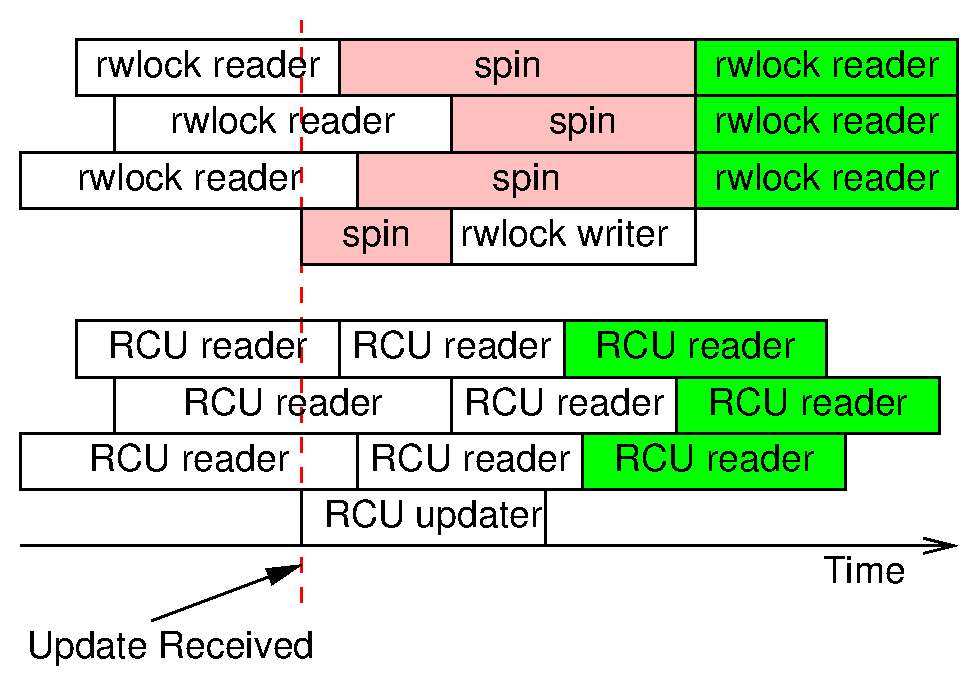
\includegraphics{defer/rwlockRCUupdate}}
\end{center}
\caption{Response Time of RCU vs. Reader-Writer Locking}
\label{fig:defer:Response Time of RCU vs. Reader-Writer Locking}
\end{figure}

However, in a surprisingly large number of situations, inconsistencies and
stale data are not problems.
The classic example is the networking routing table.
Because routing updates can take considerable time to reach a given
system (seconds or even minutes), the system will have been sending
packets the wrong way for quite some time when the update arrives.
It is usually not a problem to continue sending updates the wrong
way for a few additional milliseconds.
Furthermore, because RCU updaters can make changes without waiting for
RCU readers to finish,
the RCU readers might well see the change more quickly than would
batch-fair
reader-writer-locking readers, as shown in
Figure~\ref{fig:defer:Response Time of RCU vs. Reader-Writer Locking}.

Once the update is received, the rwlock writer cannot proceed until the
last reader completes, and subsequent readers cannot proceed until the
writer completes.
However, these subsequent readers are guaranteed to see the new value,
as indicated by the green background.
In contrast, RCU readers and updaters do not block each other, which permits
the RCU readers to see the updated values sooner.
Of course, because their execution overlaps that of the RCU updater,
\emph{all} of the RCU readers might well see updated values, including
the three readers that started before the update.
Nevertheless only the RCU readers with green backgrounds
are \emph{guaranteed} to see the updated values, again, as indicated
by the green background.

Reader-writer locking and RCU simply provide different guarantees.
With reader-writer locking, any reader that begins after the writer begins
is guaranteed to see new values, and any reader that attempts to
begin while the writer is spinning might or might not see new values,
depending on the reader/writer preference of the rwlock implementation in
question.
In contrast, with RCU, any reader that begins after the updater completes
is guaranteed to see new values, and any reader that completes after the
updater begins might or might not see new values, depending on timing.

The key point here is that, although reader-writer locking does
indeed guarantee consistency within the confines of the computer system,
there are situations where this consistency comes at the price of
increased \emph{inconsistency} with the outside world.
In other words, reader-writer locking obtains internal consistency at the
price of silently stale data with respect to the outside world.

Nevertheless, there are situations where inconsistency and stale
data within the confines of the system cannot be tolerated.
Fortunately,
there are a number of approaches that avoid inconsistency and stale
data~\cite{PaulEdwardMcKenneyPhD,Arcangeli03}, and some
methods based on reference counting are discussed in
Section~@@@.

\paragraph{Low-Priority RCU Readers Can Block High-Priority Reclaimers}

In Realtime RCU~\cite{DinakarGuniguntala2008IBMSysJ},
SRCU~\cite{PaulEMcKenney2006c}, or
QRCU~\cite{PaulEMcKenney2007QRCUspin},
each of which is described in
the final installment of this series,
a preempted reader will prevent
a grace period from completing, even if a high-priority task is
blocked waiting for that grace period to complete.
Realtime RCU can avoid this problem by substituting \url{call_rcu()}
for \url{synchronize_rcu()} or by using RCU priority
boosting~\cite{PaulEMcKenney2007BoostRCU,DinakarGuniguntala2008IBMSysJ}.
which is still in experimental status as of early 2008.
It might become necessary to augment SRCU and QRCU with priority boosting,
but not before a clear real-world need is demonstrated.

\paragraph{RCU Grace Periods Extend for Many Milliseconds}

With the exception of QRCU, RCU grace periods extend for multiple
milliseconds.
Although there are a number of techniques to render such long delays
harmless, including use of the asynchronous interfaces where available
(\url{call_rcu()} and \url{call_rcu_bh()}), this situation
is a major reason for the rule of thumb that RCU be used in read-mostly
situations.

\paragraph{Comparison of Reader-Writer Locking and RCU Code}

In the best case, the conversion from reader-writer locking to RCU
is quite simple, as shown in
Figures~\ref{fig:defer:Converting Reader-Writer Locking to RCU: Data},
\ref{fig:defer:Converting Reader-Writer Locking to RCU: Search},
and
\ref{fig:defer:Converting Reader-Writer Locking to RCU: Deletion},
all taken from
Wikipedia~\cite{WikipediaRCU}.

\begin{figure*}[htbp]
{ \scriptsize \centering
\begin{verbatim}
 1 struct el {                           1 struct el {
 2   struct list_head lp;                2   struct list_head lp;
 3   long key;                           3   long key;
 4   spinlock_t mutex;                   4   spinlock_t mutex;
 5   int data;                           5   int data;
 6   /* Other data fields */             6   /* Other data fields */
 7 };                                    7 };
 8 DEFINE_RWLOCK(listmutex);             8 DEFINE_SPINLOCK(listmutex);
 9 LIST_HEAD(head);                      9 LIST_HEAD(head);
\end{verbatim}
}
\caption{Converting Reader-Writer Locking to RCU: Data}
\label{fig:defer:Converting Reader-Writer Locking to RCU: Data}
\end{figure*}

\begin{figure*}[htbp]
{ \scriptsize \centering
\begin{verbatim}
 1 int search(long key, int *result)     1 int search(long key, int *result)
 2 {                                     2 {
 3   struct el *p;                       3   struct el *p;
 4                                       4
 5   read_lock(&listmutex);              5   rcu_read_lock();
 6   list_for_each_entry(p, &head, lp) { 6   list_for_each_entry_rcu(p, &head, lp) {
 7     if (p->key == key) {              7     if (p->key == key) {
 8       *result = p->data;              8       *result = p->data;
 9       read_unlock(&listmutex);        9       rcu_read_unlock();
10       return 1;                      10       return 1;
11     }                                11     }
12   }                                  12   }
13   read_unlock(&listmutex);           13   rcu_read_unlock();
14   return 0;                          14   return 0;
15 }                                    15 }
\end{verbatim}
}
\caption{Converting Reader-Writer Locking to RCU: Search}
\label{fig:defer:Converting Reader-Writer Locking to RCU: Search}
\end{figure*}

\begin{figure*}[htbp]
{ \scriptsize \centering
\begin{verbatim}
 1 int delete(long key)                  1 int delete(long key)
 2 {                                     2 {
 3   struct el *p;                       3   struct el *p;
 4                                       4
 5   write_lock(&listmutex);             5   spin_lock(&listmutex);
 6   list_for_each_entry(p, &head, lp) { 6   list_for_each_entry(p, &head, lp) {
 7     if (p->key == key) {              7     if (p->key == key) {
 8       list_del(&p->lp);               8       list_del_rcu(&p->lp);
 9       write_unlock(&listmutex);       9       spin_unlock(&listmutex);
                                        10       synchronize_rcu();
10       kfree(p);                      11       kfree(p);
11       return 1;                      12       return 1;
12     }                                13     }
13   }                                  14   }
14   write_unlock(&listmutex);          15   spin_unlock(&listmutex);
15   return 0;                          16   return 0;
16 }                                    17 }
\end{verbatim}
}
\caption{Converting Reader-Writer Locking to RCU: Deletion}
\label{fig:defer:Converting Reader-Writer Locking to RCU: Deletion}
\end{figure*}

More-elaborate cases of replacing reader-writer locking with RCU
are beyond the scope of this document.

\subsubsection{RCU is a Restricted Reference-Counting Mechanism}
\label{sec:defer:RCU is a Restricted Reference-Counting Mechanism}

Because grace periods are not allowed to complete while
there is an RCU read-side critical section in progress,
the RCU read-side primitives may be used as a restricted
reference-counting mechanism.
For example, consider the following code fragment:

\vspace{5pt}
\begin{minipage}[t]{\columnwidth}
\scriptsize
\begin{verbatim}
  1 rcu_read_lock();  /* acquire reference. */
  2 p = rcu_dereference(head);
  3 /* do something with p. */
  4 rcu_read_unlock();  /* release reference. */
\end{verbatim}
\end{minipage}
\vspace{5pt}

The \url{rcu_read_lock()} primitive can be thought of as
acquiring a reference to \url{p}, because a grace period
starting after the \url{rcu_dereference()} assigns to \url{p}
cannot possibly end until after we reach the matching
\url{rcu_read_unlock()}.
This reference-counting scheme is restricted in that
we are not allowed to block in RCU read-side critical sections,
nor are we permitted to hand off an RCU read-side critical section
from one task to another.

Regardless of these restrictions,
the following code can safely delete \url{p}:

\vspace{5pt}
\begin{minipage}[t]{\columnwidth}
\scriptsize
\begin{verbatim}
  1 spin_lock(\&mylock);
  2 p = head;
  3 rcu_assign_pointer(head, NULL);
  4 spin_unlock(\&mylock);
  5 /* Wait for all references to be released. */
  6 synchronize_rcu();
  7 kfree(p);
\end{verbatim}
\end{minipage}
\vspace{5pt}

The assignment to \url{head} prevents any future references
to \url{p} from being acquired, and the \url{synchronize_rcu()}
waits for any previously acquired references to be released.

\QuickQuiz{
But wait!
This is exactly the same code that might be used when thinking
of RCU as a replacement for reader-writer locking!
What gives?}
\QuickQuizAnswer{
This is an effect of the Law of Toy Examples:
beyond a certain point, the code fragments look the same.
The only difference is in how we think about the code.
However, this difference can be extremely important.
For but one example of the importance, consider that if we think
of RCU as a restricted reference counting scheme, we would never
be fooled into thinking that the updates would exclude the RCU
read-side critical sections.
\\ ~ \\
It nevertheless is often useful to think of RCU as a replacement
for reader-writer locking, for example, when you are replacing reader-writer
locking with RCU.
} \QuickQuizEnd

Of course, RCU can also be combined with traditional reference counting,
as has been discussed on LKML and as summarized in
Section~\ref{sec:defer:Reference Counting}.

\begin{figure}[tb]
\begin{center}
\resizebox{3in}{!}{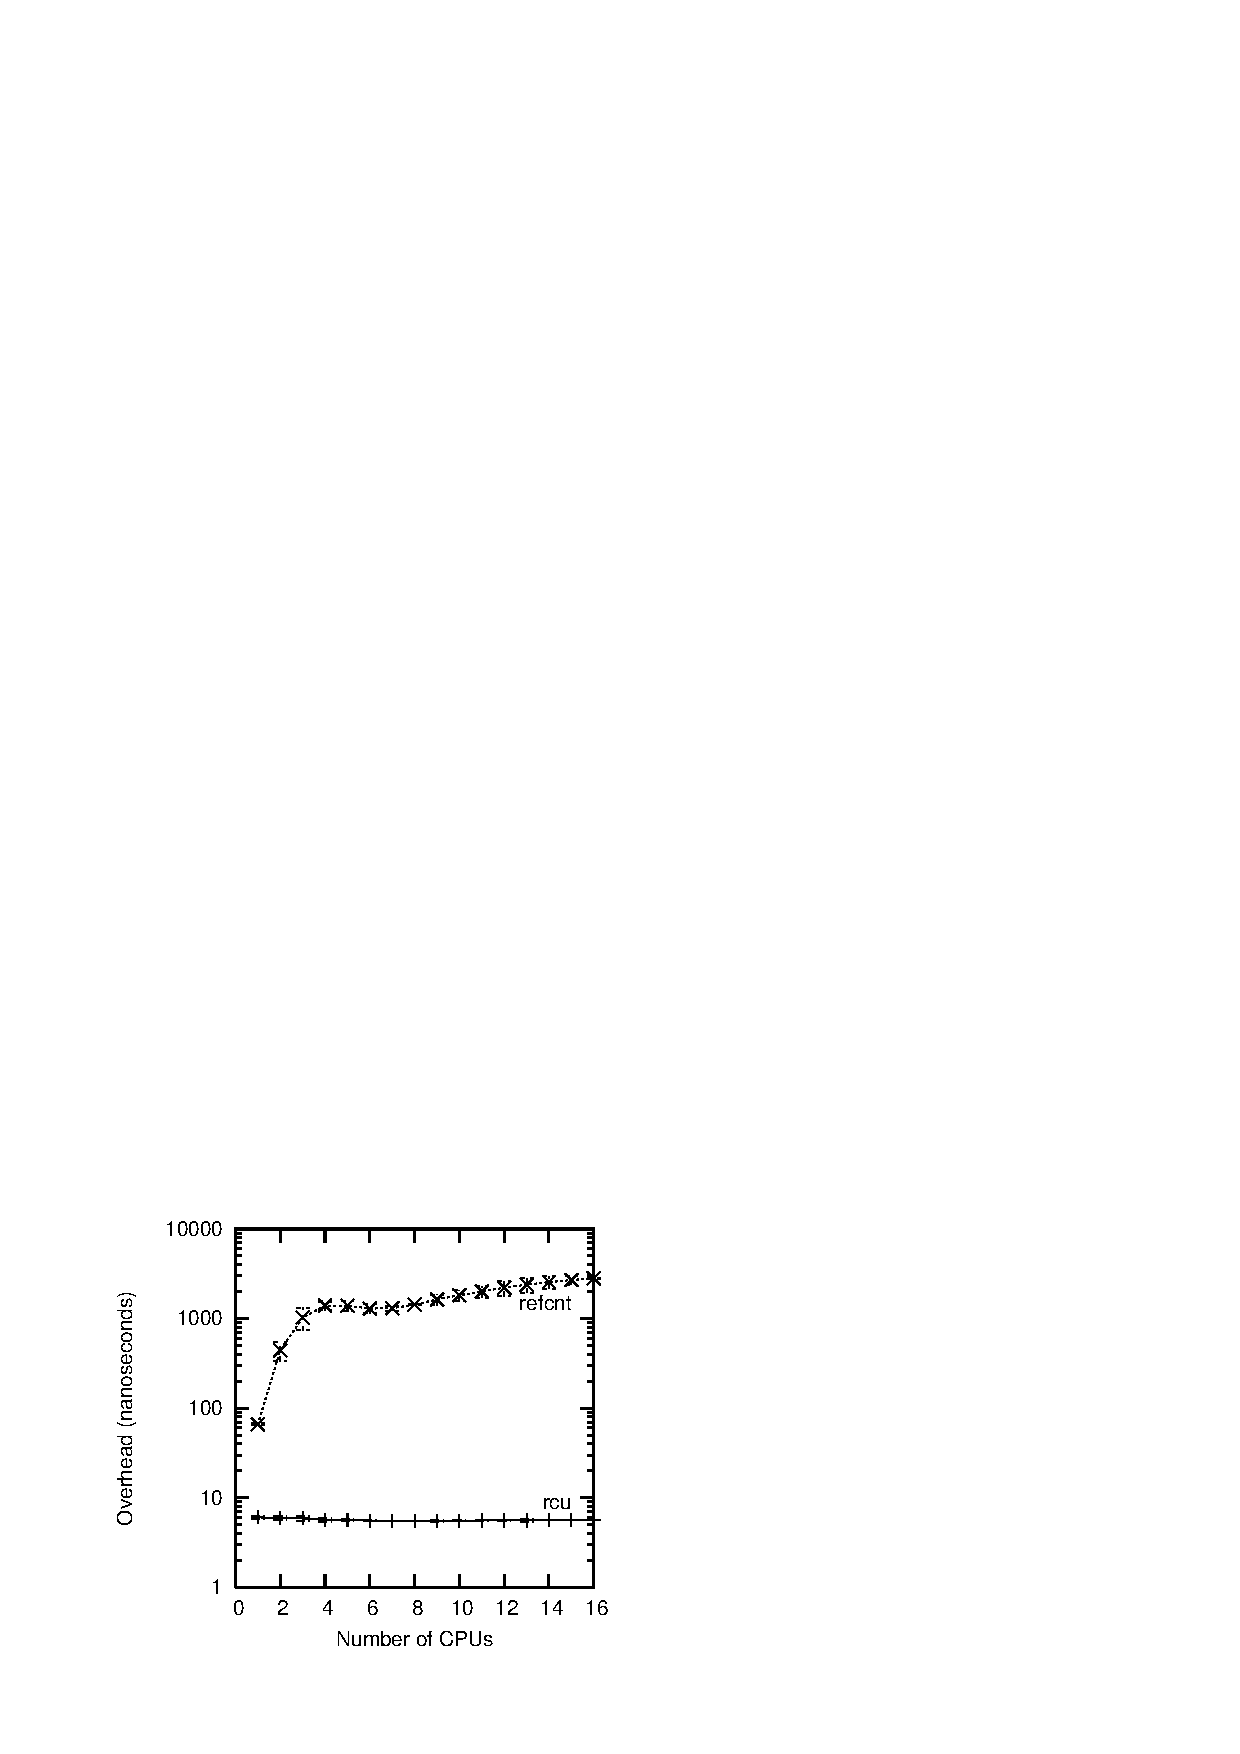
\includegraphics{defer/refRCUperfPREEMPT}}
\end{center}
\caption{Performance of RCU vs. Reference Counting}
\label{fig:defer:Performance of RCU vs. Reference Counting}
\end{figure}

But why bother?
Again, part of the answer is performance, as shown in
Figure~\ref{fig:defer:Performance of RCU vs. Reference Counting},
again showing data taken on a 16-CPU 3GHz Intel x86 system.

\QuickQuiz{
Why the dip in refcnt overhead near 6 CPUs?}
\QuickQuizAnswer{
Most likely NUMA effects.
However, there is substantial variance in the values measured for the
refcnt line, as can be seen by the error bars.
In fact, standard deviations range in excess of 10% of measured
values in some cases.
The dip in overhead therefore might well be a statistical aberration.
} \QuickQuizEnd

\begin{figure}[tb]
\begin{center}
\resizebox{3in}{!}{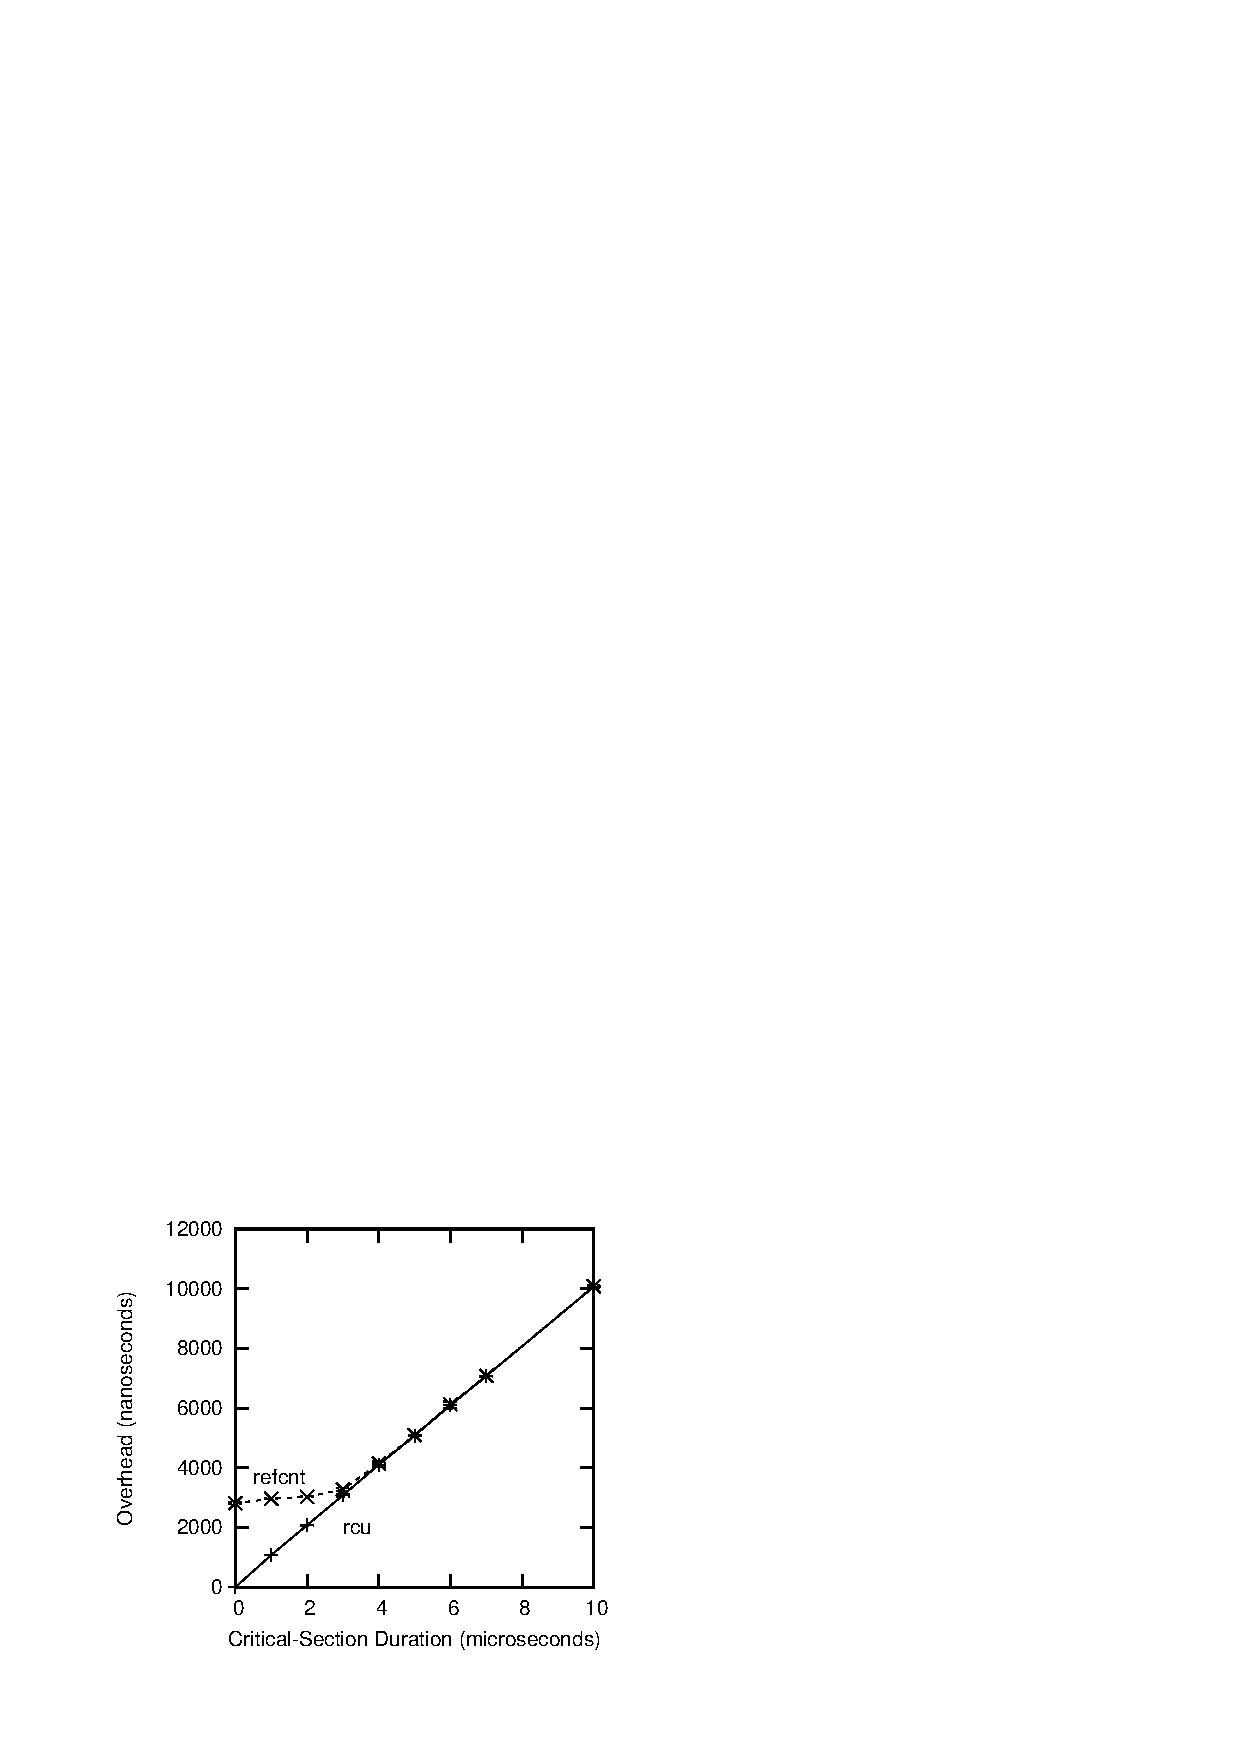
\includegraphics{defer/refRCUperfwtPREEMPT}}
\end{center}
\caption{Response Time of RCU vs. Reference Counting}
\label{fig:defer:Response Time of RCU vs. Reference Counting}
\end{figure}

And, as with reader-writer locking, the performance advantages
of RCU are most pronounced for short-duration critical sections, as shown
Figure~\ref{fig:defer:Response Time of RCU vs. Reference Counting}
for a 16-CPU system.
In addition, as with reader-writer locking, many system calls (and thus
any RCU read-side critical sections that they contain) complete in
a few microseconds.

However, the restrictions that go with RCU can be quite onerous.
For example, in many cases, the prohibition against sleeping while in an RCU
read-side critical section would defeat the entire purpose.
The next section looks at ways of addressing this problem, while also
reducing the complexity of traditional reference counting, at least in
some cases.

\subsubsection{RCU is a Bulk Reference-Counting Mechanism}
\label{sec:defer:RCU is a Bulk Reference-Counting Mechanism}

As noted in the preceding section,
traditional reference counters are usually associated with a specific
data structure, or perhaps a specific group of data structures.
However, maintaining a single global reference counter for a large
variety of data structures typically results in bouncing
the cache line containing the reference count.
Such cache-line bouncing can severely degrade performance.

In contrast, RCU's light-weight read-side primitives permit
extremely frequent read-side usage with negligible performance
degradation, permitting RCU to be used as a "bulk reference-counting"
mechanism with little or no performance penalty.
Situations where a reference must be held by a single task across a
section of code that blocks may be accommodated with
Sleepable RCU (SRCU)~\cite{PaulEMcKenney2006c}.
This fails to cover the not-uncommon situation where a reference is "passed"
from one task to another, for example, when a reference is acquired
when starting an I/O and released in the corresponding completion
interrupt handler.
(In principle, this could be handled by the SRCU implementation,
but in practice, it is not yet clear whether this is a good tradeoff.)

Of course, SRCU brings restrictions of its own, namely that the
return value from \url{srcu_read_lock()} be passed into the
corresponding \url{srcu_read_unlock()}, and that no SRCU primitives
be invoked from hardware irq handlers or from NMI/SMI handlers.
The jury is still out as to how much of a problem is presented by
these restrictions, and as to how they can best be handled.

\subsubsection{RCU is a Poor Man's Garbage Collector}
\label{sec:defer:RCU is a Poor Man's Garbage Collector}

A not-uncommon exclamation made by people first learning about
RCU is "RCU is sort of like a garbage collector!".
This exclamation has a large grain of truth, but it can also be
misleading.

Perhaps the best way to think of the relationship between RCU
and automatic garbage collectors (GCs) is that RCU resembles 
a GC in that the \emph{timing} of collection is automatically
determined, but that RCU differs from a GC in that: (1) the programmer
must manually indicate when a given data structure is eligible
to be collected, and (2) the programmer must manually mark the
RCU read-side critical sections where references might legitimately
be held.

Despite these differences, the resemblance does go quite deep,
and has appeared in at least one theoretical analysis of RCU.
Furthermore, the first RCU-like mechanism I am aware of used
a garbage collector to handle the grace periods.
Nevertheless, a better way of thinking of RCU is described in the
following section.

\subsubsection{RCU is a Way of Providing Existence Guarantees}
\label{sec:defer:RCU is a Way of Providing Existence Guarantees}

Gamsa et al.~\cite{Gamsa99}
discuss existence guarantees and describe how a mechanism
resembling RCU can be used to provide these existence guarantees
(see section~5 on page 7 of the PDF).
The effect is that if any RCU-protected data element is accessed
within an RCU read-side critical section, that data element is
guaranteed to remain in existence for the duration of that RCU
read-side critical section.

Alert readers will recognize this as only a slight variation on
the original "RCU is a way of waiting for things to finish" theme,
which is addressed in the following section.

\subsubsection{RCU is a Way of Providing Type-Safe Memory}
\label{sec:deferRCU is a Way of Providing Type-Safe Memory}

A number of lockless algorithms do not require that a given data
element keep the same identity through a given RCU read-side critical
section referencing it---but only if that data element retains the
same type.
In other words, these lockless algorithms can tolerate a given data
element being freed and reallocated as the same type of structure
while they are referencing it, but must prohibit a change in type.
This guarantee, called ``type-safe memory'' in
academic literature~\cite{Cheriton96a},
is weaker than the existence guarantees in the
previous section, and is therefore quite a bit harder to work with.
Type-safe memory algorithms in the Linux kernel make use of slab caches,
specially marking these caches so that RCU is used when returning a freed-up
slab to system memory.
This use of RCU guarantees that any in-use element of
such a slab will remain in that slab, thus retaining its type,
for the duration of any pre-existing RCU read-side critical sections.

\QuickQuiz{
	But what if there is an arbitrarily long series of RCU
	read-side critical sections in multiple threads, so that at
	any point in time there is at least one thread in the system
	executing in an RCU read-side critical section?
	Wouldn't that prevent any data from a \url{SLAB_DESTROY_BY_RCU}
	slab ever being returned to the system, possibly resulting
	in OOM events?}
\QuickQuizAnswer{
	There could certainly be an arbitrarily long period of time
	during which at least one thread is always in an RCU read-side
	critical section.
	However, the key words in the description in
	Section~\ref{sec:deferRCU is a Way of Providing Type-Safe Memory}
	are ``in-use'' and ``pre-existing''.
	Keep in mind that a given RCU read-side critical section is
	conceptually only permitted to gain references to data elements
	that were in use at the beginning of that critical section.
	Furthermore, remember that a slab cannot be returned to the
	system until all of its data elements have been freed, in fact,
	the RCU grace period cannot start until after they have all been
	freed.

	Therefore, the slab cache need only wait for those RCU read-side
	critical sections that started before the freeing of the last element
	of the slab.
	This in turn means that any RCU grace period that begins after
	the freeing of the last element will do---the slab may be returned
	to the system after that grace period ends.
} \QuickQuizEnd

These algorithms typically use a validation step that checks to make
sure that the newly referenced data structure really is the one that
was requested.
These validation checks require that portions of the data structure
remain untouched by the free-reallocate process.
Such validation checks are usually very hard to get right, and can
hide subtle and difficult bugs.

Therefore, although type-safety-based lockless algorithms can be extremely
helpful in a very few difficult situations, you should instead use existence
guarantees where possible.
Simpler is after all almost always better.

\subsubsection{RCU is a Way of Waiting for Things to Finish}
\label{sec:deferRCU is a Way of Waiting for Things to Finish}

As noted in Section~\ref{sec:defer:RCU Fundamentals}
an important component
of RCU is a way of waiting for RCU readers to finish.
One of
RCU's great strengths is that it allows you to wait for each of
thousands of different things to finish without having to explicitly
track each and every one of them, and without having to worry about
the performance degradation, scalability limitations, complex deadlock
scenarios, and memory-leak hazards that are inherent in schemes that
use explicit tracking.

In this section, we will show how \url{synchronize_sched()}'s
read-side counterparts (which include anything that disables preemption,
along with hardware operations and
primitives that disable irq) permit you to implement interactions with
non-maskable interrupt (NMI)
handlers that would be quite difficult if using locking.
This approach has been called "Pure RCU"~\cite{PaulEdwardMcKenneyPhD},
and it is used in a number of places in the Linux kernel.

The basic form of such "Pure RCU" designs is as follows:

\begin{enumerate}
\item	Make a change, for example, to the way that the OS reacts to an NMI.
\item	Wait for all pre-existing read-side critical sections to
	completely finish (for example, by using the
	\url{synchronize_sched()} primitive).
	The key observation here is that subsequent RCU read-side critical
	sections are guaranteed to see whatever change was made.
\item	Clean up, for example, return status indicating that the
	change was successfully made.
\end{enumerate}

The remainder of this section presents example code adapted from
the Linux kernel.
In this example, the \url{timer_stop} function uses
\url{synchronize_sched()} to ensure that all in-flight NMI
notifications have completed before freeing the associated resources.
A simplified version of this code is shown
Figure~\ref{fig:defer:Using RCU to Wait for NMIs to Finish}.

\begin{figure}[tbp]
{ \scriptsize
\begin{verbatim}
  1 struct profile_buffer {
  2   long size;
  3   atomic_t entry[0];
  4 };
  5 static struct profile_buffer *buf = NULL;
  6 
  7 void nmi_profile(unsigned long pcvalue)
  8 {
  9   struct profile_buffer *p = rcu_dereference(buf);
 10 
 11   if (p == NULL)
 12     return;
 13   if (pcvalue >= p->size)
 14     return;
 15   atomic_inc(\&p->entry[pcvalue]);
 16 }
 17 
 18 void nmi_stop(void)
 19 {
 20   struct profile_buffer *p = buf;
 21 
 22   if (p == NULL)
 23     return;
 24   rcu_assign_pointer(buf, NULL);
 25   synchronize_sched();
 26   kfree(p);
 27 }
\end{verbatim}
}
\caption{Using RCU to Wait for NMIs to Finish}
\label{fig:defer:Using RCU to Wait for NMIs to Finish}
\end{figure}

Lines~1-4 define a \url{profile_buffer} structure, containing a
size and an indefinite array of entries.
Line~5 defines a pointer to a profile buffer, which is
presumably initialized elsewhere to point to a dynamically allocated
region of memory.

Lines~7-16 define the \url{nmi_profile()} function,
which is called from within an NMI handler.
As such, it cannot be preempted, nor can it be interrupted by a normal
irq handler, however, it is still subject to delays due to cache misses,
ECC errors, and cycle stealing by other hardware threads within the same
core.
Line~9 gets a local pointer to the profile buffer using the
\url{rcu_dereference()} primitive to ensure memory ordering on
DEC Alpha, and
lines~11 and 12 exit from this function if there is no
profile buffer currently allocated, while lines~13 and 14
exit from this function if the \url{pcvalue} argument
is out of range.
Otherwise, line~15 increments the profile-buffer entry indexed
by the \url{pcvalue} argument.
Note that storing the size with the buffer guarantees that the
range check matches the buffer, even if a large buffer is suddenly
replaced by a smaller one.

Lines~18-27 define the \url{nmi_stop()} function,
where the caller is responsible for mutual exclusion (for example,
holding the correct lock).
Line~20 fetches a pointer to the profile buffer, and
lines~22 and 23 exit the function if there is no buffer.
Otherwise, line~24 NULLs out the profile-buffer pointer
(using the \url{rcu_assign_pointer()} primitive to maintain
memory ordering on weakly ordered machines),
and line~25 waits for an RCU Sched grace period to elapse,
in particular, waiting for all non-preemptible regions of code,
including NMI handlers, to complete.
Once execution continues at line~26, we are guaranteed that
any instance of \url{nmi_profile()} that obtained a
pointer to the old buffer has returned.
It is therefore safe to free the buffer, in this case using the
\url{kfree()} primitive.

\QuickQuiz{
Suppose that the \url{nmi_profile()} function was preemptible.
What would need to change to make this example work correctly?}
\QuickQuizAnswer{
One approach would be to use
\url{rcu_read_lock()} and \url{rcu_read_unlock()}
in \url{nmi_profile()}, and to replace the
\url{synchronize_sched()} with \url{synchronize_rcu()},
perhaps as shown in
Figure~\ref{fig:defer:Using RCU to Wait for Mythical Preemptable NMIs to Finish}.
\\ ~ \\
\begin{figure}[tbp]
{ \tt \scriptsize
\begin{verbatim}
  1 struct profile_buffer {
  2   long size;
  3   atomic_t entry[0];
  4 };
  5 static struct profile_buffer *buf = NULL;
  6 
  7 void nmi_profile(unsigned long pcvalue)
  8 {
  9   struct profile_buffer *p;
 10 
 11   rcu_read_lock();
 12   p = rcu_dereference(buf);
 13   if (p == NULL) {
 14     rcu_read_unlock();
 15     return;
 16   }
 17   if (pcvalue >= p->size) {
 18     rcu_read_unlock();
 19     return;
 20   }
 21   atomic_inc(&p->entry[pcvalue]);
 22   rcu_read_unlock();
 23 }
 24 
 25 void nmi_stop(void)
 26 {
 27   struct profile_buffer *p = buf;
 28 
 29   if (p == NULL)
 30     return;
 31   rcu_assign_pointer(buf, NULL);
 32   synchronize_rcu();
 33   kfree(p);
 34 }
\end{verbatim}
}
\caption{Using RCU to Wait for Mythical Preemptable NMIs to Finish}
\label{fig:defer:Using RCU to Wait for Mythical Preemptable NMIs to Finish}
\end{figure}

} \QuickQuizEnd

In short, RCU makes it easy to dynamically switch among profile
buffers (you just \emph{try} doing this efficiently with atomic
operations, or at all with locking!).
However, RCU is normally used at a higher level of abstraction, as
was shown in the previous sections.

\subsubsection{RCU Usage Summary}
\label{sec:defer:RCU Usage Summary}

At its core, RCU is nothing more nor less than an API that provides:

\begin{enumerate}
\item	a publish-subscribe mechanism for adding new data,
\item	a way of waiting for pre-existing RCU readers to finish, and
\item	a discipline of maintaining multiple versions to permit change
	without harming or unduly delaying concurrent RCU readers.
\end{enumerate}

That said, it is possible to build higher-level constructs
on top of RCU, including the reader-writer-locking, reference-counting,
and existence-guarantee constructs listed in the earlier sections.
Furthermore, I have no doubt that the Linux community will continue to
find interesting new uses for RCU,
as well as for any of a number of other synchronization primitives.

% <h3>Acknowledgements</h3> @@@
% 
% We are all indebted to Andy Whitcroft, Jon Walpole, and Gautham Shenoy,
% whose review of an early draft of this document greatly improved it.
% I owe thanks to the members of the Relativistic Programming project
% and to members of PNW TEC for many valuable discussions.
% I am grateful to Dan Frye for his support of this effort.

% defer/rcuAPI.tex

\subsection{RCU Linux-Kernel API}
\label{sec:defer:RCU Linux-Kernel API}

This section looks at RCU from the viewpoint of its Linux-kernel API.
Section~\ref{sec:defer:RCU has a Family of Wait-to-Finish APIs}
presents RCU's wait-to-finish APIs, and
Section~\ref{sec:defer:RCU has Publish-Subscribe and Version-Maintenance APIs}
presents RCU's publish-subscribe and version-maintenance APIs.
Finally,
Section~\ref{sec:defer:So, What is RCU Really?}
presents concluding remarks.

\subsubsection{RCU has a Family of Wait-to-Finish APIs}
\label{sec:defer:RCU has a Family of Wait-to-Finish APIs}

\begin{table*}[p]
\begin{center}
\scriptsize
\begin{tabular}{p{1.1in}|p{1.0in}|p{1.1in}|p{1.0in}|p{0.9in}}
Attribute &
    RCU Classic &
	RCU BH &
	    RCU Sched &
		Realtime RCU \\
\hline
\hline
Purpose &
    Original &
	Prevent DDoS attacks &
	    { \raggedright Wait for preempt-disable regions,
	      hardirqs, \& NMIs } &
	        Realtime response \\
\hline
Availability &
    2.5.43 &
	2.6.9 &
	    2.6.12 &
	        2.6.26 \\
\hline
Read-side primitives &
    { \raggedright
      \url{rcu_read_lock()}~! \\
      \url{rcu_read_unlock()}~! } &
	{ \raggedright
	  \url{rcu_read_lock_bh()} \\
	  \url{rcu_read_unlock_bh()} } &
	    { \raggedright
	      \url{preempt_disable()} \\
	      \url{preempt_enable()} \\
	      (and friends) } &
	        { \raggedright
		  \url{rcu_read_lock()} \\
		  \url{rcu_read_unlock()} } \\
\hline
{ Update-side primitives (synchronous) } &
    { \url{synchronize_rcu()} \url{synchronize_net()} } &
	&
	    \url{synchronize_sched()} &
	        { \url{synchronize_rcu()} \url{synchronize_net()} } \\
\hline
{ Update-side primitives (asynchronous/callback) } &
    \url{call_rcu()} ! &
	\url{call_rcu_bh()} &
	    &
	        \url{call_rcu()} \\
\hline
{ Update-side primitives (wait for callbacks) } &
    \url{rcu_barrier()} &
	\url{rcu_barrier_bh()} &
	    \url{rcu_barrier_sched()} &
	        \url{rcu_barrier()} \\
\hline
Read side constraints &
    No blocking &
	No irq enabling &
	    No blocking &
	        No blocking except preemption and lock acquisition \\
\hline
Read side overhead &
    Preempt disable/enable (free on non-PREEMPT) &
	BH disable/enable &
	    Preempt disable/enable (free on non-PREEMPT) &
	        Simple instructions, irq disable/enable \\
\hline
Asynchronous update-side overhead (for example, \url{call_rcu()}) &
    sub-microsecond &
	sub-microsecond &
	    &
	        sub-microsecond \\
\hline
Grace-period latency &
    10s of milliseconds &
	10s of milliseconds &
	    10s of milliseconds &
	        10s of milliseconds \\
\hline
Non-\url{PREEMPT_RT} implementation &
    RCU Classic &
	RCU BH &
	    RCU Classic &
	        Preemptable RCU \\
\hline
\url{PREEMPT_RT} implementation &
    Preemptable RCU &
	Realtime RCU &
	    Forced Schedule on all CPUs &
	        Realtime RCU \\
\end{tabular}
\end{center}
\caption{RCU Wait-to-Finish APIs}
\label{tab:defer:RCU Wait-to-Finish APIs}
\end{table*}

\begin{table*}[p]
\begin{center}
\scriptsize
\begin{tabular}{p{1.1in}|p{1.5in}|p{1.5in}}
Attribute &
    SRCU &
	QRCU \\
\hline
\hline
Purpose &
    Sleeping readers &
	Sleeping readers and fast grace periods \\
\hline
Availability &
    2.6.19 &
	\\
\hline
Read-side primitives &
    { \raggedright
      \url{srcu_read_lock()} \\
      \url{srcu_read_unlock()} } &
	{ \raggedright
	  \url{qrcu_read_lock()} \\
	  \url{qrcu_read_unlock()} } \\
\hline
{ Update-side primitives (synchronous) } &
    \url{synchronize_srcu()} &
	\url{synchronize_qrcu()} \\
\hline
{ Update-side primitives (asynchronous/callback) } &
    N/A &
	N/A \\
\hline
{ Update-side primitives (wait for callbacks) } &
    N/A &
	N/A \\
\hline
Read side constraints &
    No \url{synchronize_srcu()} &
	No \url{synchronize_qrcu()} \\
\hline
Read side overhead &
    Simple instructions, preempt disable/enable &
	Atomic increment and decrement of shared variable \\
\hline
Asynchronous update-side overhead (for example, \url{call_rcu()}) &
    N/A &
	N/A \\
\hline
Grace-period latency &
    10s of milliseconds &
	10s of \emph{nanoseconds} in absence of readers \\
\hline
Non-\url{PREEMPT_RT} implementation &
    SRCU &
	N/A \\
\hline
\url{PREEMPT_RT} implementation &
    SRCU &
	N/A \\
\end{tabular}
\end{center}
\caption{Sleepable RCU Wait-to-Finish APIs}
\label{tab:defer:Sleepable RCU Wait-to-Finish APIs}
\end{table*}

The most straightforward answer to ``what is RCU'' is that RCU is
an API used in the Linux kernel, as summarized by
Tables~\ref{tab:defer:RCU Wait-to-Finish APIs} and
\ref{tab:defer:Sleepable RCU Wait-to-Finish APIs},
which shows the wait-for-RCU-readers portions of the non-sleepable and
sleepable APIs, respectively,
and by
Table~\ref{tab:defer:RCU Publish-Subscribe and Version Maintenance APIs},
which shows the publish/subscribe portions of the API.

If you are new to RCU, you might consider focusing on just one
of the columns in
Table~\ref{tab:defer:RCU Wait-to-Finish APIs},
each of which summarizes one member of the Linux kernel's RCU API family..
For example, if you are primarily interested in understanding how RCU
is used in the Linux kernel, ``RCU Classic'' would be the place to start,
as it is used most frequently.
On the other hand, if you want to understand RCU for its own sake,
``SRCU'' has the simplest API.
You can always come back for the other columns later.

If you are already familiar with RCU, these tables can
serve as a useful reference.

\QuickQuiz{Why do some of the cells in
Table~\ref{tab:defer:RCU Wait-to-Finish APIs}
have exclamation marks (``!'')?}
\QuickQuizAnswer{
The green API members (\url{rcu_read_lock()},
\url{rcu_read_unlock()}, and \url{call_rcu()}) were the
only members of the Linux RCU API that Paul E. McKenney was aware of back
in the mid-90s.
During this timeframe, he was under the mistaken impression that
he knew all that there is to know about RCU.
} \QuickQuizEnd

The ``RCU Classic'' column corresponds to the original RCU implementation,
in which RCU read-side critical sections are delimited by
\url{rcu_read_lock()} and \url{rcu_read_unlock()}, which
may be nested.
The corresponding synchronous update-side primitives,
\url{synchronize_rcu()}, along with its synonym
\url{synchronize_net()}, wait for any currently executing
RCU read-side critical sections to complete.
The length of this wait is known as a ``grace period''.
The asynchronous update-side primitive, \url{call_rcu()},
invokes a specified function with a specified argument after a
subsequent grace period.
For example, \url{call_rcu(p,f);} will result in
the ``RCU callback'' \url{f(p)}
being invoked after a subsequent grace period.
There are situations,
such as when unloading a Linux-kernel module that uses \url{call_rcu()},
when it is necessary to wait for all
outstanding RCU callbacks to complete~\cite{PaulEMcKenney2007rcubarrier}.
The \url{rcu_barrier()} primitive does this job.

In the ``RCU BH'' column, \url{rcu_read_lock_bh()} and
\url{rcu_read_unlock_bh()} delimit RCU read-side critical
sections, and \url{call_rcu_bh()} invokes the specified
function and argument after a subsequent grace period.
Note that RCU BH does not have a synchronous \url{synchronize_rcu_bh()}
interface,
though one could easily be added if required.

\QuickQuiz{What happens if you mix and match?
For example, suppose you use \url{rcu_read_lock()} and
\url{rcu_read_unlock()} to delimit RCU read-side critical
sections, but then use \url{call_rcu_bh()} to post an
RCU callback?}
\QuickQuizAnswer{
If there happened to be no RCU read-side critical
sections delimited by \url{rcu_read_lock_bh()} and
\url{rcu_read_unlock_bh()} at the time \url{call_rcu_bh()}
was invoked, RCU would be within its rights to invoke the callback
immediately, possibly freeing a data structure still being used by
the RCU read-side critical section!
This is not merely a theoretical possibility: a long-running RCU
read-side critical section delimited by \url{rcu_read_lock()}
and \url{rcu_read_unlock()} is vulnerable to this failure mode.

This vulnerability disappears in -rt kernels, where
RCU Classic and RCU BH both map onto a common implementation.
} \QuickQuizEnd

In the ``RCU Sched'' column, anything that disables preemption
acts as an RCU read-side critical section, and \url{synchronize_sched()}
waits for the corresponding RCU grace period.
This RCU API family was added in the 2.6.12 kernel, which split the
old \url{synchronize_kernel()} API into the current
\url{synchronize_rcu()} (for RCU Classic) and
\url{synchronize_sched()} (for RCU Sched).
Note that RCU Sched does not have an asynchronous
\url{call_rcu_sched()} interface,
though one could be added if required.

\QuickQuiz{What happens if you mix and match RCU Classic and RCU Sched?}
\QuickQuizAnswer{
In a non-\url{PREEMPT} or a \url{PREEMPT} kernel, mixing these
two works "by accident" because in those kernel builds, RCU Classic and RCU
Sched map to the same implementation.
However, this mixture is fatal in \url{PREEMPT_RT} builds using the -rt
patchset, due to the fact that Realtime RCU's read-side critical
sections can be preempted, which would permit
\url{synchronize_sched()} to return before the
RCU read-side critical section reached its \url{rcu_read_unlock()}
call.
This could in turn result in a data structure being freed before the
read-side critical section was finished with it,
which could in turn greatly increase the actuarial risk experienced
by your kernel.

In fact, the split between RCU Classic and RCU Sched was inspired
by the need for preemptible RCU read-side critical sections.
} \QuickQuizEnd

The ``Realtime RCU'' column has the same API as does
RCU Classic, the only difference being that RCU read-side critical
sections may be preempted and may block while acquiring spinlocks.
The design of Realtime RCU is described
elsewhere~\cite{PaulEMcKenney2007PreemptibleRCU}.

\QuickQuiz{Why do both SRCU and QRCU lack asynchronous \url{call_srcu()}
or \url{call_qrcu()} interfaces?}
\QuickQuizAnswer{
Given an asynchronous interface, a single task
could register an arbitrarily large number of SRCU or QRCU callbacks,
thereby consuming an arbitrarily large quantity of memory.
In contrast, given the current synchronous
\url{synchronize_srcu()} and \url{synchronize_qrcu()}
interfaces, a given task must finish waiting for a given grace period
before it can start waiting for the next one.
} \QuickQuizEnd

The ``SRCU'' column displays a specialized RCU API that permits
general sleeping in RCU read-side critical sections
(see Appendix~\ref{app:Sleepable Read-Copy Update} for more details).
Of course,
use of \url{synchronize_srcu()} in an SRCU read-side
critical section can result in
self-deadlock, so should be avoided.
SRCU differs from earlier RCU implementations in that the caller
allocates an \url{srcu_struct} for each distinct SRCU
usage.
This approach prevents SRCU read-side critical sections from blocking
unrelated \url{synchronize_srcu()} invocations.
In addition, in this variant of RCU, \url{srcu_read_lock()}
returns a value that must be passed into the corresponding
\url{srcu_read_unlock()}.

The ``QRCU'' column presents an RCU implementation with the same
API structure as SRCU, but optimized for extremely low-latency
grace periods in absence of readers, as described
elsewhere~\cite{PaulEMcKenney2007QRCUspin}.
As with SRCU, use of \url{synchronize_qrcu()} can result in
self-deadlock, so should be avoided.
Although QRCU has not yet been accepted into the Linux kernel, it
is worth mentioning given that it is the only RCU implementation
that can boast deep sub-microsecond grace-period latencies.

\QuickQuiz{Under what conditions can \url{synchronize_srcu()} be safely
used within an SRCU read-side critical section?}
\QuickQuizAnswer{
In principle, you can use
\url{synchronize_srcu()} with a given \url{srcu_struct}
within an SRCU read-side critical section that uses some other
\url{srcu_struct}.
In practice, however, doing this is almost certainly a bad idea.
In particular, the following could still result in deadlock:
\\
\vspace{5pt}
\begin{minipage}[t]{\columnwidth}
{\tt
~~1 idx = srcu\_read\_lock(\&ssa);\\
~~2 synchronize\_srcu(\&ssb);\\
~~3 srcu\_read\_unlock(\&ssa, idx);\\
~~4 \\
~~5 /* . . . */\\
~~6 \\
~~7 idx = srcu\_read\_lock(\&ssb);\\
~~8 synchronize\_srcu(\&ssa);\\
~~9 srcu\_read\_unlock(\&ssb, idx);\\
}
\end{minipage}

} \QuickQuizEnd

The Linux kernel currently has a surprising number of RCU APIs and
implementations.
There is some hope of reducing this number, evidenced by the fact
that a given build of the Linux kernel currently has at most
three implementations behind four APIs (given that RCU Classic
and Realtime RCU share the same API).
However, careful inspection and analysis will be required, just as
would be required for one of the many locking APIs.

\subsubsection{RCU has Publish-Subscribe and Version-Maintenance APIs}
\label{sec:defer:RCU has Publish-Subscribe and Version-Maintenance APIs}

Fortunately, the RCU publish-subscribe and version-maintenance
primitives shown in the following
table apply to all of the variants of RCU discussed above.
This commonality can in some cases allow more code to be shared,
which certainly reduces the API proliferation that would otherwise
occur.

\begin{table*}[tb]
\begin{center}
% \scriptsize
\begin{tabular}{p{1.1in}|p{1.9in}|p{0.7in}|p{1.3in}}
Category &
	Primitives &
		Availability &
			Overhead \\
\hline
\hline
List traversal &
	\url{list_for_each_entry_rcu()} &
		2.5.59 &
			{ \raggedright
			  Simple instructions (memory barrier on Alpha) } \\
\hline
List update &
	\url{list_add_rcu()} &
		2.5.44 &
			Memory barrier \\
&
	\url{list_add_tail_rcu()} &
		2.5.44 &
			Memory barrier \\
&
	\url{list_del_rcu()} &
		2.5.44 &
			Simple instructions \\
&
	\url{list_replace_rcu()} &
		2.6.9 &
			Memory barrier \\
&
	\url{list_splice_init_rcu()} &
		2.6.21 &
			Grace-period latency \\
\hline
Hlist traversal &
	\url{hlist_for_each_entry_rcu()} &
		2.6.8 &
			{ \raggedright
			  Simple instructions (memory barrier on Alpha) } \\
&
	\url{hlist_add_after_rcu()} &
		2.6.14 &
			Memory barrier \\
&
	\url{hlist_add_before_rcu()} &
		2.6.14 &
			Memory barrier \\
&
	\url{hlist_add_head_rcu()} &
		2.5.64 &
			Memory barrier \\
&
	\url{hlist_del_rcu()} &
		2.5.64 &
			Simple instructions \\
&
	\url{hlist_replace_rcu()} &
		2.6.15 &
			Memory barrier \\
\hline
Pointer traversal &
	\url{rcu_dereference()} &
		2.6.9 &
			{ \raggedright
			  Simple instructions (memory barrier on Alpha) } \\
\hline
Pointer update &
	\url{rcu_assign_pointer()} &
		2.6.10 &
			Memory barrier \\
\end{tabular}
\end{center}
\caption{RCU Publish-Subscribe and Version Maintenance APIs}
\label{tab:defer:RCU Publish-Subscribe and Version Maintenance APIs}
\end{table*}

The first pair of categories operate on Linux
\url{struct}~\url{list_head} lists, which are circular, doubly-linked
lists.
The \url{list_for_each_entry_rcu()} primitive traverses an
RCU-protected list in a type-safe manner, while also enforcing
memory ordering for situations where a new list element is inserted
into the list concurrently with traversal.
On non-Alpha platforms, this primitive incurs little or no performance
penalty compared to \url{list_for_each_entry()}.
The \url{list_add_rcu()}, \url{list_add_tail_rcu()},
and \url{list_replace_rcu()} primitives are analogous to
their non-RCU counterparts, but incur the overhead of an additional
memory barrier on weakly-ordered machines.
The \url{list_del_rcu()} primitive is also analogous to its
non-RCU counterpart, but oddly enough is very slightly faster due to the
fact that it poisons only the \url{prev} pointer rather than
both the \url{prev} and \url{next} pointers as
\url{list_del()} must do.
Finally, the \url{list_splice_init_rcu()} primitive is similar
to its non-RCU counterpart, but incurs a full grace-period latency.
The purpose of this grace period is to allow RCU readers to finish
their traversal of the source list before completely disconnecting
it from the list header -- failure to do this could prevent such
readers from ever terminating their traversal.

\QuickQuiz{Why doesn't \url{list_del_rcu()} poison both the \url{next}
and \url{prev} pointers?}
\QuickQuizAnswer{
Poisoning the \url{next} pointer would interfere
with concurrent RCU readers, who must use this pointer.
However, RCU readers are forbidden from using the \url{prev}
pointer, so it may safely be poisoned.
} \QuickQuizEnd

The second pair of categories operate on Linux's
\url{struct}~\url{hlist_head}, which is a linear linked list.
One advantage of \url{struct}~\url{hlist_head} over
\url{struct}~\url{list_head} is that the former requires only
a single-pointer list header, which can save significant memory in
large hash tables.
The \url{struct}~\url{hlist_head} primitives in the table
relate to their non-RCU counterparts in much the same way as do the
\url{struct}~\url{list_head} primitives.

The final pair of categories operate directly on pointers, and
are useful for creating RCU-protected non-list data structures,
such as RCU-protected arrays and trees.
The \url{rcu_assign_pointer()} primitive ensures that any
prior initialization remains ordered before the assignment to the
pointer on weakly ordered machines.
Similarly, the \url{rcu_dereference()} primitive ensures that subsequent
code dereferencing the pointer will see the effects of initialization code
prior to the corresponding \url{rcu_assign_pointer()} on
Alpha CPUs.
On non-Alpha CPUs, \url{rcu_dereference()} documents which pointer
dereferences are protected by RCU.

\QuickQuiz{Normally, any pointer subject to \url{rcu_dereference()} \emph{must}
always be updated using \url{rcu_assign_pointer()}.
What is an exception to this rule?}
\QuickQuizAnswer{
One such exception is when a multi-element linked
data structure is initialized as a unit while inaccessible to other
CPUs, and then a single \url{rcu_assign_pointer()} is used
to plant a global pointer to this data structure.
The initialization-time pointer assignments need not use
\url{rcu_assign_pointer()}, though any such assignments that
happen after the structure is globally visible \url{must} use
\url{rcu_assign_pointer()}.
\\
However, unless this initialization code is on an impressively hot
code-path, it is probably wise to use \url{rcu_assign_pointer()}
anyway, even though it is in theory unnecessary.
It is all too easy for a "minor" change to invalidate your cherished
assumptions about the initialization happening privately.
} \QuickQuizEnd

\QuickQuiz{Are there any downsides to the fact that these traversal and update
primitives can be used with any of the RCU API family members?}
\QuickQuizAnswer{
It can sometimes be difficult for automated
code checkers such as "sparse" (or indeed for human beings) to
work out which type of RCU read-side critical section a given
RCU traversal primitive corresponds to.
For example, consider the following:
\\
\vspace{5pt}
\begin{minipage}[t]{\columnwidth}
{ \tt
~~1 rcu\_read\_lock();\\
~~2 preempt\_disable();\\
~~3 p = rcu\_dereference(global\_pointer);\\
~~4 \\
~~5 /* . . . */\\
~~6 \\
~~7 preempt\_enable();\\
~~8 rcu\_read\_unlock();\\
}
\end{minipage}
\vspace{5pt}
\\
Is the \url{rcu_dereference()} primitive in an RCU Classic
or an RCU Sched critical section?
What would you have to do to figure this out?
} \QuickQuizEnd

\subsubsection{So, What \emph{is} RCU Really?}
\label{sec:defer:So, What is RCU Really?}

At its core, RCU is nothing more nor less than an API that supports
publication and subscription for insertions, waiting for all RCU readers
to complete, and maintenance of multiple versions.
That said, it is possible to build higher-level constructs
on top of RCU, including the reader-writer-locking, reference-counting,
and existence-guarantee constructs listed in the companion article.
Furthermore, I have no doubt that the Linux community will continue to
find interesting new uses for RCU,
just as they do for any of a number of synchronization
primitives throughout the kernel.

Finally, a complete view of RCU would also include
all of the things you can do with these APIs.

% Acknowledgements @@@

% We are all indebted to Andy Whitcroft, Jon Walpole, and Gautham Shenoy,
% whose review of an early draft of this document greatly improved it.
% I owe thanks to the members of the Relativistic Programming project
% and to members of PNW TEC for many valuable discussions.
% I am grateful to Dan Frye for his support of this effort.
%
% Also those commenting on the LWN article.

% defer/toyrcu.tex

\subsection{``Toy'' RCU Implementations}
\label{defer:``Toy'' RCU Implementations}

The toy RCU implementations in this section are designed not for
high performance, practicality, or any kind of production use,
but rather for clarity.
Nevertheless, you will need a thorough understanding of
Chapters~\ref{chp:Introduction} and
\ref{chp:defer:Deferred Processing}
for even these toy RCU implementations to be easily understandable.

Section~\ref{defer:Lock-Based RCU} presents a rudimentary
RCU implementation based on simple locking, while
Section~\ref{defer:Simple Counter-Based RCU} through
\ref{defer:Scalable Counter-Based RCU With Shared Grace Periods}
present a series of
simple RCU implementations based on locking, reference counters,
and free-running counters.

\subsubsection{Lock-Based RCU}
\label{defer:Lock-Based RCU}

\begin{figure}[bp]
{ \scriptsize
\begin{verbatim}
  1 static void rcu_read_lock(void)
  2 {
  3   spin_lock(&rcu_gp_lock);
  4 }
  5 
  6 static void rcu_read_unlock(void)
  7 {
  8   spin_unlock(&rcu_gp_lock);
  9 }
 10 
 11 void synchronize_rcu(void)
 12 {
 13   spin_lock(&rcu_gp_lock);
 14   spin_unlock(&rcu_gp_lock);
 15 }
\end{verbatim}
}
\caption{Lock-Based RCU Implementation}
\label{fig:defer:Lock-Based RCU Implementation}
\end{figure}

Perhaps the simplest RCU implementation leverages locking, as
shown in
Figure~\ref{fig:defer:Lock-Based RCU Implementation}
(\url{rcu_lock.h} and \url{rcu_lock.c}).
In this implementation, \url{rcu_read_lock()} acquires a global
spinlock, \url{rcu_read_unlock()} releases it, and
\url{synchronize_rcu()} acquires it then immediately releases it.

Because \url{synchronize_rcu()} does not return until it has acquired
(and released) the lock, it cannot return until all prior RCU read-side
critical sections have completed, thus faithfully implementing
RCU semantics.
Of course, only one RCU reader may be in its read-side critical section
at a time, which almost entirely defeats the purpose of RCU.
In addition, the lock operations in \url{rcu_read_lock()} and
\url{rcu_read_unlock()} are extremely heavyweight,
with read-side overhead ranging from about 100~nanoseconds on a single Power5
CPU up to more than 17~\emph{microseconds} on a 64-CPU system.
Worse yet,
these same lock operations permit \url{rcu_read_lock()}
to participate in deadlock cycles.
Furthermore, in absence of recursive locks, 
RCU read-side critical sections cannot be nested, and, finally,
although concurrent RCU updates could in principle be satisfied by
a common grace period, this implementation serializes grace periods,
preventing grace-period sharing.

\QuickQuiz{}
	Why wouldn't any deadlock in the RCU implementation in
	Figure~\ref{fig:defer:Lock-Based RCU Implementation}
	also be a deadlock in any other RCU implementation?
\QuickQuizAnswer{

\begin{figure}[tbp]
{ \scriptsize
\begin{verbatim}
  1 void foo(void)
  2 {
  3   spin_lock(&my_lock);
  4   rcu_read_lock();
  5   do_something();
  6   rcu_read_unlock();
  7   do_something_else();
  8   spin_unlock(&my_lock);
  9 }
 10 
 11 void bar(void)
 12 {
 13   rcu_read_lock();
 14   spin_lock(&my_lock);
 15   do_some_other_thing();
 16   spin_unlock(&my_lock);
 17   do_whatever();
 18   rcu_read_unlock();
 19 }
\end{verbatim}
}
\caption{Deadlock in Lock-Based RCU Implementation}
\label{fig:defer:Deadlock in Lock-Based RCU Implementation}
\end{figure}

	Suppose the functions \url{foo()} and \url{bar()} in
	Figure~\ref{fig:defer:Deadlock in Lock-Based RCU Implementation}
	are invoked concurrently from different CPUs.
	Then \url{foo()} will acquire \url{my_lock()} on line~3,
	while \url{bar()} will acquire \url{rcu_gp_lock} on
	line~13.
	When \url{foo()} advances to line~4, it will attempt to
	acquire \url{rcu_gp_lock}, which is held by \url{bar()}.
	Then when \url{bar()} advances to line~14, it will attempt
	to acquire \url{my_lock}, which is held by \url{foo()}.

	Each function is then waiting for a lock that the other
	holds, a classic deadlock.

	Other RCU implementations neither spin nor block in
	\url{rcu_read_lock()}, hence avoiding deadlocks.
} \QuickQuizEnd

\QuickQuiz{}
	Why not simply use reader-writer locks in the RCU implementation
	in
	Figure~\ref{fig:defer:Lock-Based RCU Implementation}
	in order to allow RCU readers to proceed in parallel?
\QuickQuizAnswer{
	One could in fact use reader-writer locks in this manner.
	However, textbook reader-writer locks suffer from memory
	contention, so that the RCU read-side critical sections would
	need to be quite long to actually permit parallel execution.
	@@@ add reference to reader-writer locking discussion from LJ2003 @@@

	On the other hand, use of a reader-writer lock that is
	read-acquired in \url{rcu_read_lock()} would avoid the
	deadlock condition noted above.
} \QuickQuizEnd

It is hard to imagine this implementation being useful
in a production setting, though it does have the virtue
of being implementable in almost any user-level application.
Furthermore, similar implementations having one lock per CPU
or using reader-writer locks have been used in production
in the 2.4 Linux kernel.

A modified version of this one-lock-per-CPU approach, but instead using
one lock per thread, is described
in the next section.

\subsubsection{Per-Thread Lock-Based RCU}
\label{defer:Per-Thread Lock-Based RCU}

\begin{figure}[bp]
{ \scriptsize
\begin{verbatim}
  1 static void rcu_read_lock(void)
  2 {
  3   spin_lock(&__get_thread_var(rcu_gp_lock));
  4 }
  5 
  6 static void rcu_read_unlock(void)
  7 {
  8   spin_unlock(&__get_thread_var(rcu_gp_lock));
  9 }
 10 
 11 void synchronize_rcu(void)
 12 {
 13   int t;
 14 
 15   for_each_running_thread(t) {
 16     spin_lock(&per_thread(rcu_gp_lock, t));
 17     spin_unlock(&per_thread(rcu_gp_lock, t));
 18   }
 19 }
\end{verbatim}
}
\caption{Per-Thread Lock-Based RCU Implementation}
\label{fig:defer:Per-Thread Lock-Based RCU Implementation}
\end{figure}

Figure~\ref{fig:defer:Per-Thread Lock-Based RCU Implementation}
(\url{rcu_lock_percpu.h} and \url{rcu_lock_percpu.c})
shows an implementation based on one lock per thread.
The \url{rcu_read_lock()} and \url{rcu_read_unlock()} functions
acquire and release, respectively, the current thread's lock.
The \url{synchronize_rcu()} function acquires and releases each thread's
lock in turn.
Therefore, all RCU read-side critical sections running
when \url{synchronize_rcu()} starts must have completed before
\url{synchronize_rcu()} can return.

This implementation does have the virtue of permitting concurrent
RCU readers, and does avoid the deadlock condition that can arise
with a single global lock.
Furthermore, the read-side overhead, though high at roughly 140 nanoseconds,
remains at about 140 nanoseconds regardless of the number of CPUs.
However, the update-side overhead ranges from about 600 nanoseconds
on a single Power5 CPU
up to more than 100 \emph{microseconds} on 64 CPUs.

\QuickQuiz{}
	Wouldn't it be cleaner to acquire all the locks, and then
	release them all in the loop from lines~15-18 of
	Figure~\ref{fig:defer:Per-Thread Lock-Based RCU Implementation}?
	After all, with this change, there would be a point in time
	when there were no readers, simplifying things greatly.
\QuickQuizAnswer{
	Making this change would re-introduce the deadlock, so
	no, it would not be cleaner.
} \QuickQuizEnd

\QuickQuiz{}
	Is the implementation shown in
	Figure~\ref{fig:defer:Per-Thread Lock-Based RCU Implementation}
	free from deadlocks?
	Why or why not?
\QuickQuizAnswer{
	One deadlock is where a lock is
	held across \url{synchronize_rcu()}, and that same lock is
	acquired within an RCU read-side critical section.
	However, this situation will deadlock any correctly designed
	RCU implementation.
	After all, the \url{synchronize_rcu()} primitive must wait for all
	pre-existing RCU read-side critical sections to complete,
	but if one of those critical sections is spinning on a lock
	held by the thread executing the \url{synchronize_rcu()},
	we have a deadlock inherent in the definition of RCU.

	Another deadlock happens when attempting to nest RCU read-side
	critical sections.
	This deadlock is peculiar to this implementation, and might
	be avoided by using recursive locks, or by using reader-writer
	locks that are read-acquired by \url{rcu_read_lock()} and
	write-acquired by \url{synchronize_rcu()}.

	However, if we exclude the above two cases,
	this implementation of RCU does not introduce any deadlock
	situations.
	This is because only time some other thread's lock is acquired is when
	executing \url{synchronize_rcu()}, and in that case, the lock
	is immediately released, prohibiting a deadlock cycle that
	does not involve a lock held across the \url{synchronize_rcu()}
	which is the first case above.
} \QuickQuizEnd

The counter-based RCU implementation described next overcomes some of
the shortcomings of the lock-based implementation.

\subsubsection{Simple Counter-Based RCU}
\label{defer:Simple Counter-Based RCU}

\begin{figure}[tbp]
{ \scriptsize
\begin{verbatim}
  1 atomic_t rcu_refcnt;
  2 
  3 static void rcu_read_lock(void)
  4 {
  5   atomic_inc(&rcu_refcnt);
  6   smp_mb();
  7 }
  8 
  9 static void rcu_read_unlock(void)
 10 {
 11   smp_mb();
 12   atomic_dec(&rcu_refcnt);
 13 }
 14 
 15 void synchronize_rcu(void)
 16 {
 17   smp_mb();
 18   while (atomic_read(&rcu_refcnt) != 0) {
 19     poll(NULL, 0, 10);
 20   }
 21   smp_mb();
 22 }
\end{verbatim}
}
\caption{RCU Implementation Using Single Global Reference Counter}
\label{fig:defer:RCU Implementation Using Single Global Reference Counter}
\end{figure}

A slightly more sophisticated RCU implementation is shown in
Figure~\ref{fig:defer:RCU Implementation Using Single Global Reference Counter}
(\url{rcu_rcg.h} and \url{rcu_rcg.c}).
This implementation makes use of a global reference counter
\url{rcu_refcnt} defined on line~1.
The \url{rcu_read_lock()} primitive atomically increments this
counter, then executes a memory barrier to ensure that the
RCU read-side critical section is ordered after the atomic
increment.
Similarly, \url{rcu_read_unlock()} executes a memory barrier to
confine the RCU read-side critical section, then atomically
decrements the counter.
The \url{synchronize_rcu()} primitive spins waiting for the reference
counter to reach zero, surrounded by memory barriers.
The \url{poll()} on line~19 merely provides pure delay, and from
a pure RCU-semantics point of view could be omitted.
Again, once \url{synchronize_rcu()} returns, all prior
RCU read-side critical sections are guaranteed to have completed.

In happy contrast to the lock-based implementation shown in
Section~\ref{defer:Lock-Based RCU}, this implementation
allows parallel execution of RCU read-side critical sections.
In happy contrast to the per-thread lock-based implementation shown in
Section~\ref{defer:Per-Thread Lock-Based RCU},
it also allows them to be nested.
In addition, the \url{rcu_read_lock()} primitive cannot possibly
participate in deadlock cycles, as it never spins nor blocks.

\QuickQuiz{}
	But what if you hold a lock across a call to
	\url{synchronize_rcu()}, and then acquire that same lock within
	an RCU read-side critical section?
\QuickQuizAnswer{
	Indeed, this would deadlock any legal RCU implementation.
	But is \url{rcu_read_lock()} \emph{really} participating in
	the deadlock cycle?
	If you believe that it is, then please
	ask yourself this same question when looking at the
	RCU implementation in
	Section~\ref{defer:RCU Based on Quiescent States}.
} \QuickQuizEnd

However, this implementations still has some serious shortcomings.
First, the atomic operations in \url{rcu_read_lock()} and
\url{rcu_read_unlock()} are still quite  heavyweight,
with read-side overhead ranging from about 100~nanoseconds on
a single Power5 CPU up to almost 40~\emph{microseconds}
on a 64-CPU system.
This means that the RCU read-side critical sections
have to be extremely long in order to get any real
read-side parallelism.
On the other hand, in the absence of readers, grace periods elapse
in about 40~\emph{nanoseconds}, many orders of magnitude faster
than production-quality implementations in the Linux kernel.

\QuickQuiz{}
	How can the grace period possibly elapse in 40 nanoseconds when
	\url{synchronize_rcu()} contains a 10-millisecond delay?
\QuickQuizAnswer{
	The update-side test was run in absence of readers, so the
	\url{poll()} system call was never invoked.
	In addition, the actual code has this \url{poll()}
	system call commented out, the better to evaluate the
	true overhead of the update-side code.
	Any production uses of this code would be better served by
	using the \url{poll()} system call, but then again,
	production uses would be even better served by other implementations
	shown later in this section.
} \QuickQuizEnd

Second, if there are many concurrent \url{rcu_read_lock()}
and \url{rcu_read_unlock()} operations, there will
be extreme memory contention on \url{rcu_refcnt},
resulting in expensive cache misses.
Both of these first two shortcomings largely defeat a major purpose of
RCU, namely to provide low-overhead read-side synchronization primitives.

Third, a large number of RCU readers with long read-side
critical sections could prevent \url{synchronize_rcu()}
from ever completing, as the global counter might
never reach zero.
This could result in starvation of RCU updates, which
is of course unacceptable in production settings.

Finally, although concurrent RCU updates could in principle be
satisfied by a common grace period, this implementation
serializes grace periods, preventing grace-period
sharing.

\QuickQuiz{}
	Why not simply make \url{rcu_read_lock()} wait when a concurrent
	\url{synchronize_rcu()} has been waiting too long in
	the RCU implementation in
	Figure~\ref{fig:defer:RCU Implementation Using Single Global Reference Counter}?
	Wouldn't that prevent \url{synchronize_rcu()} from starving?
\QuickQuizAnswer{
	Although this would in fact eliminate the starvation, it would
	also mean that \url{rcu_read_lock()} would spin or block waiting
	for the writer, which is in turn waiting on readers.
	If one of these readers is attempting to acquire a lock that
	the spinning/blocking \url{rcu_read_lock()} holds, we again
	have deadlock.

	In short, the cure is worse than the disease.
	See Section~\ref{defer:Starvation-Free Counter-Based RCU}
	for a proper cure.
} \QuickQuizEnd

Therefore, it is still hard to imagine this implementation being useful
in a production setting, though it has a bit more potential
than the lock-based mechanism, for example, as an RCU implementation
suitable for a high-stress debugging environment.
The next section describes a variation on the reference-counting
scheme that is more favorable to writers.

\subsubsection{Starvation-Free Counter-Based RCU}
\label{defer:Starvation-Free Counter-Based RCU}

\begin{figure}[tbp]
{ \scriptsize
\begin{verbatim}
  1 static void rcu_read_lock(void)
  2 {
  3   int i;
  4   int n;
  5 
  6   n = __get_thread_var(rcu_nesting);
  7   if (n == 0) {
  8     i = atomic_read(&rcu_idx);
  9     __get_thread_var(rcu_read_idx) = i;
 10     atomic_inc(&rcu_refcnt[i]);
 11   }
 12   __get_thread_var(rcu_nesting) = n + 1;
 13   smp_mb();
 14 }
 15 
 16 static void rcu_read_unlock(void)
 17 {
 18   int i;
 19   int n;
 20 
 21   smp_mb();
 22   n = __get_thread_var(rcu_nesting);
 23   if (n == 1) {
 24      i = __get_thread_var(rcu_read_idx);
 25     atomic_dec(&rcu_refcnt[i]);
 26   }
 27   __get_thread_var(rcu_nesting) = n - 1;
 28 }
\end{verbatim}
}
\caption{RCU Read-Side Using Global Reference-Count Pair}
\label{fig:defer:RCU Read-Side Using Global Reference-Count Pair}
\end{figure}

Figure~\ref{fig:defer:RCU Read-Side Using Global Reference-Count Pair}
(\url{rcu_rcgp.h})
shows the read-side primitives of an RCU implementation that uses a pair
of reference counters (\url{rcu_refcnt[]}),
along with a global index that
selects one counter out of the pair (\url{rcu_idx}),
a per-thread nesting counter \url{rcu_nesting},
a per-thread snapshot of the global index (\url{rcu_read_idx}),
and a global lock (\url{rcu_gp_lock}).

The \url{rcu_read_lock()} primitive atomically increments the member of the
\url{rcu_refcnt[]} pair indexed by \url{rcu_idx}, and keeps a
snapshot of this index in the per-thread variable \url{rcu_read_idx}.
The \url{rcu_read_unlock()} primitive then atomically decrements
whichever counter of the pair that the corresponding \url{rcu_read_lock()}
incremented.
However, because only one value of \url{rcu_idx} is remembered per thread,
additional measures must be taken to permit nesting.
These additional measures use the per-thread \url{rcu_nesting} variable
to track nesting.

To make all this work, line~6 of \url{rcu_read_lock()} in
Figure~\ref{fig:defer:RCU Read-Side Using Global Reference-Count Pair}
picks up the
current thread's instance of \url{rcu_nesting}, and if line~7 finds
that this is the outermost \url{rcu_read_lock()},
then lines~8-10 pick up the current value of
\url{rcu_idx}, save it in this thread's instance of \url{rcu_read_idx},
and atomically increment the selected element of \url{rcu_refcnt}.
Regardless of the value of \url{rcu_nesting}, line~12 increments it.
Line~13 executes a memory barrier to ensure that the RCU read-side
critical section does not bleed out before the \url{rcu_read_lock()} code.

Similarly, the \url{rcu_read_unlock()} function executes a memory barrier
at line~21
to ensure that the RCU read-side critical section does not bleed out
after the \url{rcu_read_unlock()} code.
Line~22 picks up this thread's instance of \url{rcu_nesting}, and if
line~23 finds that this is the outermost \url{rcu_read_unlock()},
then lines~24 and 25 pick up this thread's instance of \url{rcu_read_idx}
(saved by the outermost \url{rcu_read_lock()}) and atomically decrements
the selected element of \url{rcu_refcnt}.
Regardless of the nesting level, line~27 decrements this thread's
instance of \url{rcu_nesting}.

\begin{figure}[tbp]
{ \scriptsize
\begin{verbatim}
  1 void synchronize_rcu(void)
  2 {
  3   int i;
  4 
  5   smp_mb();
  6   spin_lock(&rcu_gp_lock);
  7   i = atomic_read(&rcu_idx);
  8   atomic_set(&rcu_idx, !i);
  9   smp_mb();
 10   while (atomic_read(&rcu_refcnt[i]) != 0) {
 11     poll(NULL, 0, 10);
 12   }
 13   smp_mb();
 14   atomic_set(&rcu_idx, i);
 15   smp_mb();
 16   while (atomic_read(&rcu_refcnt[!i]) != 0) {
 17     poll(NULL, 0, 10);
 18   }
 19   spin_unlock(&rcu_gp_lock);
 20   smp_mb();
 21 }
\end{verbatim}
}
\caption{RCU Update Using Global Reference-Count Pair}
\label{fig:defer:RCU Update Using Global Reference-Count Pair}
\end{figure}

Figure~\ref{fig:defer:RCU Update Using Global Reference-Count Pair}
(\url{rcu_rcpg.c})
shows the corresponding \url{synchronize_rcu()} implementation.
Lines~6 and 19 acquire and release \url{rcu_gp_lock} in order to
prevent more than one concurrent instance of \url{synchronize_rcu()}.
Lines~7-8 pick up the value of \url{rcu_idx} and complement it,
respectively, so that subsequent instances of \url{rcu_read_lock()}
will use a different element of \url{rcu_idx} that did preceding
instances.
Lines~10-12 then wait for the prior element of \url{rcu_idx} to
reach zero, with the memory barrier on line~9 ensuring that the check
of \url{rcu_idx} is not reordered to precede the complementing of
\url{rcu_idx}.
Lines~13-18 repeat this process, and line~20 ensures that any
subsequent reclamation operations are not reordered to precede the
checking of \url{rcu_refcnt}.

\QuickQuiz{}
	Why the memory barrier on line~5 of \url{synchronize_rcu()} in
	Figure~\ref{fig:defer:RCU Update Using Global Reference-Count Pair}
	given that there is a spin-lock acquisition immediately after?
\QuickQuizAnswer{
	The spin-lock acquisition only guarantees that the spin-lock's
	critical section will not ``bleed out'' to precede the
	acquisition.
	It in no way guarantees that code preceding the spin-lock
	acquisitoin won't be reordered into the critical section.
	Such reordering could cause a removal from an RCU-protected
	list to be reordered to follow the complementing of
	\url{rcu_idx}, which could allow a newly starting RCU
	read-side critical section to see the recently removed
	data element.

	Exercise for the reader: use a tool such as Promela/spin
	to determine which (if any) of the memory barriers in
	Figure~\ref{fig:defer:RCU Update Using Global Reference-Count Pair}
	are really needed.
	See Section~\ref{app:formal:Formal Verification}
	for information on using these tools.
	The first correct and complete response will be credited.
} \QuickQuizEnd

\QuickQuiz{}
	Why is the counter flipped twice in
	Figure~\ref{fig:defer:RCU Update Using Global Reference-Count Pair}?
	Shouldn't a single flip-and-wait cycle be sufficient?
\QuickQuizAnswer{
	Both flips are absolutely required.
	To see this, consider the following sequence of events:
	\begin{enumerate}
	\item	Line~8 of \url{rcu_read_lock()} in
		Figure~\ref{fig:defer:RCU Read-Side Using Global Reference-Count Pair}
		picks up \url{rcu_idx}, finding its value to be zero.
	\item	Line~8 of \url{synchronize_rcu()} in
		Figure~\ref{fig:defer:RCU Update Using Global Reference-Count Pair}
		complements the value of \url{rcu_idx}, setting its
		value to one.
	\item	Lines~10-13 of \url{synchronize_rcu()} find that the
		value of \url{rcu_refcnt[0]} is zero, and thus
		returns.
		(Recall that the question is asking what happens if
		lines~14-20 are omitted.)
	\item	Lines~9 and 10 of \url{rcu_read_lock()} store the
		value zero to this thread's instance of \url{rcu_read_idx}
		and increments \url{rcu_refcnt[0]}, respectively.
		Execution then proceeds into the RCU read-side critical
		section.
		\label{defer:rcu_rcgp:RCU Read Side Start}
	\item	Another instance of \url{synchronize_rcu()} again complements
		\url{rcu_idx}, this time setting its value to zero.
		Because \url{rcu_refcnt[1]} is zero, \url{synchronize_rcu()}
		returns immediately.
		(Recall that \url{rcu_read_lock()} incremented
		\url{rcu_refcnt[0]}, not \url{rcu_refcnt[1]}!)
		\label{defer:rcu_rcgp:RCU Grace Period Start}
	\item	The grace period that started in
		step~\ref{defer:rcu_rcgp:RCU Grace Period Start}
		has been allowed to end, despite
		the fact that the RCU read-side critical section
		that started beforehand in
		step~\ref{defer:rcu_rcgp:RCU Read Side Start}
		has not completed.
		This violates RCU semantics, and could allow the update
		to free a data element that the RCU read-side critical
		section was still referencing.
	\end{enumerate}

	Exercise for the reader: What happens if \url{rcu_read_lock()}
	is preempted for a very long time (hours!) just after
	line~8?
	Does this implementation operate correctly in that case?
	Why or why not?
	The first correct and complete response will be credited.
} \QuickQuizEnd

This implementation avoids the update-starvation issues that could
occur in the single-counter implementation shown in
Figure~\ref{fig:defer:RCU Implementation Using Single Global Reference Counter}.

There are still some serious shortcomings.
First, the atomic operations in \url{rcu_read_lock()}
and \url{rcu_read_unlock()}
are still quite heavyweight.
In fact, they are more complex than those
of the single-counter variant shown in
Figure~\ref{fig:defer:RCU Implementation Using Single Global Reference Counter},
with the read-side primitives consuming about 150~nanoseconds on a single
Power5 CPU and almost 40~\emph{microseconds} on a 64-CPU system.
The updates-side \url{synchronize_rcu()} primitive is more costly as
well, ranging from about 200~nanoseconds on a single Power5 CPU to
more than 40~\emph{microseconds} on a 64-CPU system.
This means that the RCU read-side critical sections
have to be extremely long in order to get any real
read-side parallelism.

Second, if there are many concurrent \url{rcu_read_lock()}
and \url{rcu_read_unlock()} operations, there will
be extreme memory contention on the \url{rcu_refcnt}
elements, resulting in expensive cache misses.
This further extends the RCU read-side critical-section
duration required to provide parallel read-side access.
These first two shortcomings defeat the purpose of RCU in most
situations.

Third, the need to flip \url{rcu_idx} twice imposes substantial
overhead on updates, especially if there are large
numbers of threads.

Finally, despite the fact that concurrent RCU updates could in principle be
satisfied by a common grace period, this implementation
serializes grace periods, preventing grace-period
sharing.

\QuickQuiz{}
	Given that atomic increment and decrement are so expensive,
	why not just use non-atomic increment on line~10 and a
	non-atomic decrement on line~25 of
	Figure~\ref{fig:defer:RCU Read-Side Using Global Reference-Count Pair}?
\QuickQuizAnswer{
	Using non-atomic operations would cause increments and decrements
	to be lost, in turn causing the implementation to fail.
	See Section~\ref{defer:Scalable Counter-Based RCU}
	for a safe way to use non-atomic operations in
	\url{rcu_read_lock()} and \url{rcu_read_unlock()}.
} \QuickQuizEnd

Despite these shortcomings, one could imagine this variant
of RCU being used on small tightly coupled multiprocessors,
perhaps as a memory-conserving implementation that maintains
API compatibility with more complex implementations.
However, it would not not likely scale well beyond a few CPUs.

The next section describes yet another variation on the reference-counting
scheme that provides greatly improved read-side performance and scalability.

\subsubsection{Scalable Counter-Based RCU}
\label{defer:Scalable Counter-Based RCU}

\begin{figure}[tbp]
{ \scriptsize
\begin{verbatim}
  1 static void rcu_read_lock(void)
  2 {
  3   int i;
  4   int n;
  5 
  6   n = __get_thread_var(rcu_nesting);
  7   if (n == 0) {
  8     i = atomic_read(&rcu_idx);
  9     __get_thread_var(rcu_read_idx) = i;
 10     __get_thread_var(rcu_refcnt)[i]++;
 11   }
 12   __get_thread_var(rcu_nesting) = n + 1;
 13   smp_mb();
 14 }
 15 
 16 static void rcu_read_unlock(void)
 17 {
 18   int i;
 19   int n;
 20 
 21   smp_mb();
 22   n = __get_thread_var(rcu_nesting);
 23   if (n == 1) {
 24      i = __get_thread_var(rcu_read_idx);
 25     __get_thread_var(rcu_refcnt)[i]--;
 26   }
 27   __get_thread_var(rcu_nesting) = n - 1;
 28 }
\end{verbatim}
}
\caption{RCU Read-Side Using Per-Thread Reference-Count Pair}
\label{fig:defer:RCU Read-Side Using Per-Thread Reference-Count Pair}
\end{figure}

Figure~\ref{fig:defer:RCU Read-Side Using Per-Thread Reference-Count Pair}
(\url{rcu_rcpl.h})
shows the read-side primitives of an RCU implementation that uses per-thread
pairs of reference counters.
This implementation is quite similar to that shown in
Figure~\ref{fig:defer:RCU Read-Side Using Global Reference-Count Pair},
the only difference being that \url{rcu_refcnt} is now a per-thread
variable, so the \url{rcu_read_lock()} and
\url{rcu_read_unlock()} primitives no longer perform atomic operations.

\QuickQuiz{}
	Come off it!
	We can see the \url{atomic_read()} primitive in
	\url{rcu_read_lock()}!!!
	So why are you trying to pretend that \url{rcu_read_lock()}
	contains no atomic operations???
\QuickQuizAnswer{
	The \url{atomic_read()} primitives does not actually execute
	atomic machine instructions, but rather does a normal load
	from an \url{atomic_t}.
	Its sole purpose is to keep the compiler's type-checking happy.
} \QuickQuizEnd

\begin{figure}[tbp]
{ \scriptsize
\begin{verbatim}
  1 static void flip_counter_and_wait(int i)
  2 {
  3   int t;
  4 
  5   atomic_set(&rcu_idx, !i);
  6   smp_mb();
  7   for_each_thread(t) {
  8     while (per_thread(rcu_refcnt, t)[i] != 0) {
  9       poll(NULL, 0, 10);
 10     }
 11   }
 12   smp_mb();
 13 }
 14 
 15 void synchronize_rcu(void)
 16 {
 17   int i;
 18 
 19   smp_mb();
 20   spin_lock(&rcu_gp_lock);
 21   i = atomic_read(&rcu_idx);
 22   flip_counter_and_wait(i);
 23   flip_counter_and_wait(!i);
 24   spin_unlock(&rcu_gp_lock);
 25   smp_mb();
 26 }
\end{verbatim}
}
\caption{RCU Update Using Per-Thread Reference-Count Pair}
\label{fig:defer:RCU Update Using Per-Thread Reference-Count Pair}
\end{figure}

Figure~\ref{fig:defer:RCU Update Using Per-Thread Reference-Count Pair}
(\url{rcu_rcpl.c})
shows the implementation of \url{synchronize_rcu()}, along with a helper
function named \url{flip_counter_and_wait()}.
The \url{synchronize_rcu()} function resembles that shown in
Figure~\ref{fig:defer:RCU Update Using Global Reference-Count Pair},
except that the repeated counter flip is replaced by a pair of calls
on lines~22 and 23 to the new helper function.

The new \url{flip_counter_and_wait()} function updates the
\url{rcu_idx} variable on line~5, executes a memory barrier on line~6,
then lines~7-11 spin on each thread's prior \url{rcu_refcnt} element,
waiting for it to go to zero.
Once all such elements have gone to zero,
it executes another memory barrier on line~12 and returns.

This RCU implementation imposes important new requirements on its
software environment, namely, (1) that it be possible to declare
per-thread variables, (2) that these per-thread variables be accessible
from other threads, and (3) that it is possible to enumerate all threads.
These requirements can be met in almost all software environments,
but often result in fixed upper bounds on the number of threads.
More-complex implementations might avoid such bounds, for example, by using
expandable hash tables.
Such implementations might dynamically track threads, for example, by
adding them on their first call to \url{rcu_read_lock()}.

\QuickQuiz{}
	Great, if we have $N$ threads, we can have $2N$ ten-millisecond
	waits (one set per \url{flip_counter_and_wait()} invocation,
	and even that assumes that we wait only once for each thread.
	Don't we need the grace period to complete \emph{much} more quickly?
\QuickQuizAnswer{
	Keep in mind that we only wait for a given thread if that thread
	is still in a pre-existing RCU read-side critical section,
	and that waiting for one hold-out thread gives all the other
	threads a chance to complete any pre-existing RCU read-side
	critical sections that they might still be executing.
	So the only way that we would wait for $2N$ intervals
	would be if the last thread still remained in a pre-existing
	RCU read-side critical section despite all the waiting for
	all the prior threads.
	In short, this implementation will not wait unnecessarily.

	However, if you are stress-testing code that uses RCU, you
	might want to comment out the \url{poll()} statement in
	order to better catch bugs that incorrectly retain a reference
	to an RCU-protected data element outside of an RCU
	read-side critical section.
} \QuickQuizEnd

This implementation still has several shortcomings.
First, the need to flip \url{rcu_idx} twice imposes substantial overhead
on updates, especially if there are large numbers of threads.

Second, \url{synchronize_rcu()} must now examine a number of variables
that increases linearly with the number of threads, imposing substantial
overhead on applications with large numbers of threads.

Third, as before, although concurrent RCU updates could in principle
be satisfied by a common grace period, this implementation serializes
grace periods, preventing grace-period sharing.

Finally, as noted in the text, the need for per-thread variables
and for enumerating threads may be problematic in some software
environments.

That said, the read-side primitives scale very nicely, requiring about
115~nanoseconds regardless of whether running on a single-CPU or a 64-CPU
Power5 system.
As noted above, the \url{synchronize_rcu()} primitive does not scale,
ranging in overhead from almost a microsecond on a single Power5 CPU
up to almost 200~microseconds on a 64-CPU system.
this implementation could conceivably form the basis for a
production-quality user-level RCU implementation.

The next section describes an algorithm permitting more efficient
concurrent RCU updates.

\subsubsection{Scalable Counter-Based RCU With Shared Grace Periods}
\label{defer:Scalable Counter-Based RCU With Shared Grace Periods}

\begin{figure}[tbp]
{ \scriptsize
\begin{verbatim}
  1 static void rcu_read_lock(void)
  2 {
  3   int i;
  4   int n;
  5 
  6   n = __get_thread_var(rcu_nesting);
  7   if (n == 0) {
  8     i = ACCESS_ONCE(rcu_idx) & 0x1;
  9     __get_thread_var(rcu_read_idx) = i;
 10     __get_thread_var(rcu_refcnt)[i]++;
 11   }
 12   __get_thread_var(rcu_nesting) = n + 1;
 13   smp_mb();
 14 }
 15 
 16 static void rcu_read_unlock(void)
 17 {
 18   int i;
 19   int n;
 20 
 21   smp_mb();
 22   n = __get_thread_var(rcu_nesting);
 23   if (n == 1) {
 24      i = __get_thread_var(rcu_read_idx);
 25     __get_thread_var(rcu_refcnt)[i]--;
 26   }
 27   __get_thread_var(rcu_nesting) = n - 1;
 28 }
\end{verbatim}
}
\caption{RCU Read-Side Using Per-Thread Reference-Count Pair and Shared Update}
\label{fig:defer:RCU Read-Side Using Per-Thread Reference-Count Pair and Shared Update}
\end{figure}

Figure~\ref{fig:defer:RCU Read-Side Using Per-Thread Reference-Count Pair and Shared Update}
(\url{rcu_rcpls.h})
shows the read-side primitives for an RCU implementation using per-thread
reference count pairs, as before, but permitting updates to share
grace periods.
The main difference from the earlier implementation shown in
Figure~\ref{fig:defer:RCU Read-Side Using Per-Thread Reference-Count Pair}
is that \url{rcu_idx} is now a \url{long} that counts freely,
so that line~8 of
Figure~\ref{fig:defer:RCU Read-Side Using Per-Thread Reference-Count Pair and Shared Update}
must mask off the low-order bit.
We also switched from using \url{atomic_read()} and \url{atomic_set()}
to using \url{ACCESS_ONCE()}.

\begin{figure}[tbp]
{ \scriptsize
\begin{verbatim}
  1 static void flip_counter_and_wait(int ctr)
  2 {
  3   int i;
  4   int t;
  5 
  6   ACCESS_ONCE(rcu_idx) = ctr + 1;
  7   i = ctr & 0x1;
  8   smp_mb();
  9   for_each_thread(t) {
 10     while (per_thread(rcu_refcnt, t)[i] != 0) {
 11       poll(NULL, 0, 10);
 12     }
 13   }
 14   smp_mb();
 15 }
 16 
 17 void synchronize_rcu(void)
 18 {
 19   int ctr;
 20   int oldctr;
 21 
 22   smp_mb();
 23   oldctr = ACCESS_ONCE(rcu_idx);
 24   smp_mb();
 25   spin_lock(&rcu_gp_lock);
 26   ctr = ACCESS_ONCE(rcu_idx);
 27   if (ctr - oldctr >= 3) {
 28     spin_unlock(&rcu_gp_lock);
 29     smp_mb();
 30     return;
 31   }
 32   flip_counter_and_wait(ctr);
 33   if (ctr - oldctr < 2)
 34     flip_counter_and_wait(ctr + 1);
 35   spin_unlock(&rcu_gp_lock);
 36   smp_mb();
 37 }
\end{verbatim}
}
\caption{RCU Shared Update Using Per-Thread Reference-Count Pair}
\label{fig:defer:RCU Shared Update Using Per-Thread Reference-Count Pair}
\end{figure}

Figure~\ref{fig:defer:RCU Shared Update Using Per-Thread Reference-Count Pair}
(\url{rcu_rcpls.c})
shows the implementation of \url{synchronize_rcu()} and its helper
function \url{flip_counter_and_wait()}.
These are similar to those in
Figure~\ref{fig:defer:RCU Update Using Per-Thread Reference-Count Pair}.
The differences in \url{flip_counter_and_wait()} include:
\begin{enumerate}
\item	Line~6 uses \url{ACCESS_ONCE()} instead of \url{atomic_set()},
	and increments rather than complementing.
\item	A new line~7 masks the counter down to its bottom bit.
\end{enumerate}

The changes to \url{synchronize_rcu()} are more pervasive:
\begin{enumerate}
\item	There is a new \url{oldctr} local variable that captures
	the pre-lock-acquisition value of \url{rcu_idx} on
	line~23.
\item	Line~26 uses \url{ACCESS_ONCE()} instead of \url{atomic_read()}.
\item	Lines~27-30 check to see if at least three counter flips were
	performed by other threads while the lock was being acquired,
	and, if so, releases the lock, does a memory barrier, and returns.
	In this case, there were two full waits for the counters to
	go to zero, so those other threads already did all the required work.
\item	At lines~33-34, \url{flip_counter_and_wait()} is only
	invoked a second time if there were fewer than two counter flips
	while the lock was being acquired.
	On the other hand, if there were two counter flips, some other
	thread did one full wait for all the counters to go to zero,
	so only one more is required.
\end{enumerate}

With this approach, if an arbitrarily large number of threads invoke
\url{synchronize_rcu()} concurrently, with one CPU for each thread, there
will be a total of only three waits for counters to go to zero.

Despite the improvements, this implementation of RCU still
has a few shortcomings.
First, as before, the need to flip \url{rcu_idx} twice imposes substantial
overhead on updates, especially if there are large
numbers of threads.

Second, each updater still acquires \url{rcu_gp_lock}, even if there
is no work to be done.
This can result in a severe scalability limitation
if there are large numbers of concurrent updates.
Section~\ref{app:rcuimpl:Preemptable RCU} shows
one way to avoid this in a production-quality real-time
implementation of RCU for the Linux kernel.

Third, this implementation requires per-thread variables
and the ability to enumerate threads, which again can be
problematic in some software environments.

Finally, on 32-bit machines, a given update thread might be
preempted long enough for the \url{rcu_idx}
counter to overflow.
This could cause such a thread to force an unnecessary
pair of counter flips.
However, even if each grace period took only one
microsecond, the offending thread would need to be
preempted for more than an hour, in which case an
extra pair of counter flips is likely the least of
your worries.

As with the implementation described in
Section~\ref{defer:Simple Counter-Based RCU},
the read-side primitives scale extremely well, incurring roughly
115~nanoseconds of overhead regardless of the number of CPUs.
The \url{synchronize_rcu()} primitives is still expensive,
ranging from about one microsecond up to about 16~microseconds.
This is nevertheless much cheaper than the roughly 200~microseconds
incurred by the implementation in
Section~\ref{defer:Scalable Counter-Based RCU}.
So, despite its shortcomings, one could imagine this
RCU implementation being used in production in real-life applications.

\QuickQuiz{}
	All of these toy RCU implementations have either atomic operations
	in \url{rcu_read_lock()} and \url{rcu_read_unlock()},
	or \url{synchronize_rcu()}
	overhead that increases linearly with the number of threads.
	Under what circumstances could an RCU implementation enjoy
	light-weight implementations for all three of these primitives,
	all having deterministic ($O(1)$) overheads and latencies?
\QuickQuizAnswer{
	Special-purpose uniprocessor implementations of RCU can attain
	this ideal.
	See @@@.
} \QuickQuizEnd

Referring back to
Figure~\ref{fig:defer:RCU Read-Side Using Per-Thread Reference-Count Pair and Shared Update},
we see that there is one global-variable access and no fewer than four
accesses to thread-local variables.
Given the relatively high cost of thread-local accesses on systems
implementing POSIX threads, it is tempting to collapse the three
thread-local variables into a single structure, permitting
\url{rcu_read_lock()} and \url{rcu_read_unlock()} to access their
thread-local data with a single thread-local-storage access.
However, an even better approach would be to reduce the number of
thread-local accesses to one, as is done in the next section.

\subsubsection{RCU Based on Free-Running Counter}
\label{defer:RCU Based on Free-Running Counter}

\begin{figure}[tbp]
{ \scriptsize
\begin{verbatim}
  1 static void rcu_read_lock(void)
  2 {
  3   __get_thread_var(rcu_reader_gp) = rcu_gp_ctr + 1;
  4   smp_mb();
  5 }
  6 
  7 static void rcu_read_unlock(void)
  8 {
  9   smp_mb();
 10   __get_thread_var(rcu_reader_gp) = rcu_gp_ctr;
 11 }
 12 
 13 void synchronize_rcu(void)
 14 {
 15   int t;
 16 
 17   smp_mb();
 18   spin_lock(&rcu_gp_lock);
 19   rcu_gp_ctr += 2;
 20   smp_mb();
 21   for_each_thread(t) {
 22     while ((per_thread(rcu_reader_gp, t) & 0x1) &&
 23            ((per_thread(rcu_reader_gp, t) -
 24              rcu_gp_ctr) < 0)) {
 25       poll(NULL, 0, 10);
 26     }
 27   }
 28   spin_unlock(&rcu_gp_lock);
 29   smp_mb();
 30 }
\end{verbatim}
}
\caption{Free-Running Counter Using RCU}
\label{fig:defer:Free-Running Counter Using RCU}
\end{figure}

Figure~\ref{fig:defer:Free-Running Counter Using RCU}
(\url{rcu.h} and \url{rcu.c})
show an RCU implementation based on a single global free-running counter
that takes on only even-numbered values.
The resulting \url{rcu_read_lock()} implementation is extremely
straightforward.
Line~3 simply adds one to the global free-running \url{rcu_gp_ctr}
variable and stores the resulting odd-numbered value into the
\url{rcu_reader_gp} per-thread variable.
Line~4 executes a memory barrier to prevent the content of the
subsequent RCU read-side critical section from ``leaking out''.

The \url{rcu_read_unlock()} implementation is similar.
Line~9 executes a memory barrier, again to prevent the prior RCU
read-side critical section from ``leaking out''.
Line~10 then copies the \url{rcu_gp_ctr} global variable to the
\url{rcu_reader_gp} per-thread variable, leaving this per-thread
variable with an even-numbered value so that a concurrent instance
of \url{synchronize_rcu()} will know to ignore it.

\QuickQuiz{}
	If any even value is sufficient to tell \url{synchronize_rcu()}
	to ignore a given task, why doesn't line~10 of
	Figure~\ref{fig:defer:Free-Running Counter Using RCU}
	simply assign zero to \url{rcu_reader_gp}?
\QuickQuizAnswer{
	Assigning zero (or any other even-numbered constant)
	would in fact work, but assigning the value of
	\url{rcu_gp_ctr} can provide a valuable debugging aid,
	as it gives the developer an idea of when the corresponding
	thread last exited an RCU read-side critical section.
} \QuickQuizEnd

Thus, \url{synchronize_rcu()} could wait for all of the per-thread
\url{rcu_reader_gp} variables to take on even-numbered values.
However, it is possible to do much better than that because
\url{synchronize_rcu()} need only wait on \emph{pre-existing}
RCU read-side critical sections.
Line~17 executes a memory barrier to prevent prior manipulations
of RCU-protected data structures from being reordered (by either
the CPU or the compiler) to follow the increment on line~17.
Line~18 acquires the \url{rcu_gp_lock} (and line~28 releases it)
in order to prevent multiple
\url{synchronize_rcu()} instances from running concurrently.
Line~19 then increments the global \url{rcu_gp_ctr} variable by
two, so that all pre-existing RCU read-side critical sections will
have corresponding per-thread \url{rcu_reader_gp} variables with
values less than that of \url{rcu_gp_ctr}, modulo the machine's
word size.
Recall also that threads with even-numbered values of \url{rcu_reader_gp}
are not in an RCU read-side critical section,
so that lines~21-27 scan the \url{rcu_reader_gp} values until they
all are either even (line~22) or are greater than the global
\url{rcu_gp_ctr} (lines~23-24).
Line~25 blocks for a short period of time to wait for a
pre-existing RCU read-side critical section, but this can be replaced with
a spin-loop if grace-period latency is of the essence.
Finally, the memory barrier at line~29 ensures that any subsequent
destruction will not be reordered into the preceding loop.

\QuickQuiz{}
	Why are the memory barriers on lines~17 and 29 of
	Figure~\ref{fig:defer:Free-Running Counter Using RCU}
	needed?
	Aren't the memory barriers inherent in the locking
	primitives on lines~18 and 28 sufficient?
\QuickQuizAnswer{
	These memory barriers are required because the locking
	primitives are only guaranteed to confine the critical
	section.
	The locking primitives are under absolutely no obligation
	to keep other code from bleeding in to the critical section.
	The pair of memory barriers are therefore requires to prevent
	this sort of code motion, whether performed by the compiler
	or by the CPU.
} \QuickQuizEnd

This approach achieves much better read-side performance, incurring
roughly 63~nanoseconds of overhead regardless of the number of
Power5 CPUs.
Updates incur more overhead, ranging from about 500~nanoseconds on
a single Power5 CPU to more than 100~\emph{microseconds} on 64
such CPUs.

\QuickQuiz{}
	Couldn't the update-side optimization described in
	Section~\ref{defer:Scalable Counter-Based RCU With Shared Grace Periods}
	be applied to the implementation shown in
	Figure~\ref{fig:defer:Free-Running Counter Using RCU}?
\QuickQuizAnswer{
	Indeed it could, with a few modifications.
	This work is left as an exercise for the reader.
} \QuickQuizEnd

This implementation suffers from some serious shortcomings in
addition to the high update-side overhead noted earlier.
First, it is no longer permissible to nest RCU read-side critical
sections, a topic that is taken up in the next section.
Second and finally, this implementation requires that the enclosing software
environment be able to enumerate threads and maintain per-thread
variables.

\subsubsection{Nestable RCU Based on Free-Running Counter}
\label{defer:Nestable RCU Based on Free-Running Counter}

\begin{figure}[tbp]
{ \scriptsize
\begin{verbatim}
  1 static void rcu_read_lock(void)
  2 {
  3   long tmp;
  4   long *rrgp;
  5 
  6   rrgp = &__get_thread_var(rcu_reader_gp);
  7   tmp = *rrgp;
  8   if ((tmp & RCU_GP_CTR_NEST_MASK) == 0)
  9     tmp = rcu_gp_ctr;
 10   tmp++;
 11   *rrgp = tmp;
 12   smp_mb();
 13 }
 14 
 15 static void rcu_read_unlock(void)
 16 {
 17   long tmp;
 18 
 19   smp_mb();
 20   __get_thread_var(rcu_reader_gp)--;
 21 }
 22 
 23 void synchronize_rcu(void)
 24 {
 25   int t;
 26 
 27   smp_mb();
 28   spin_lock(&rcu_gp_lock);
 29   rcu_gp_ctr += RCU_GP_CTR_BOTTOM_BIT;
 30   smp_mb();
 31   for_each_thread(t) {
 32     while (rcu_gp_ongoing(t) &&
 33            ((per_thread(rcu_reader_gp, t) -
 34              rcu_gp_ctr) < 0)) {
 35       poll(NULL, 0, 10);
 36     }
 37   }
 38   spin_unlock(&rcu_gp_lock);
 39   smp_mb();
 40 }
\end{verbatim}
}
\caption{Nestable RCU Using a Free-Running Counter}
\label{fig:defer:Nestable RCU Using a Free-Running Counter}
\end{figure}

Figure~\ref{fig:defer:Nestable RCU Using a Free-Running Counter}
(\url{rcu_nest.h} and \url{rcu_nest.c})
show an RCU implementation based on a single global free-running counter,
but that permits nesting of RCU read-side critical sections.
This nestability is accomplished by reserving the low-order bits of the
global \url{rcu_gp_ctr} to count nesting.
This is a generalization of the scheme in
Section~\ref{defer:RCU Based on Free-Running Counter},
which can be thought of as having a single low-order bit reserved
for counting nesting depth.
Two C-preprocessor macros are used to arrange this,
\url{RCU_GP_CTR_NEST_MASK} and
\url{RCU_GP_CTR_BOTTOM_BIT}.
These are related: \url{RCU_GP_CTR_NEST_MASK=RCU_GP_CTR_BOTTOM_BIT-1}.
The \url{RCU_GP_CTR_BOTTOM_BIT} macro contains a single bit that is
positioned just above the bits reserved for counting nesting,
and the \url{RCU_GP_CTR_NEST_MASK} has all one bits covering the
region of \url{rcu_gp_ctr} used to count nesting.
Obviously, these two C-preprocessor macros must reserve enough
of the low-order bits of the counter to permit the maximum required
nesting of RCU read-side critical sections, and this implementation
reserves seven bits, for a maximum RCU read-side critical-section
nesting depth of 127, which should be well in excess of that needed
by most applications.

The resulting \url{rcu_read_lock()} implementation is still reasonably
straightforward.
Line~6 places a pointer to this thread's instance of \url{rcu_reader_gp}
into the local variable \url{rrgp}, minimizing the number of expensive
calls to the pthreads thread-local-state API.
Line~7 records the current value of \url{rcu_reader_gp} into another
local variable \url{tmp}, and line~8 checks to see if the low-order
bits are zero, which would indicate that this is the outermost
\url{rcu_read_lock()}.
If so, line~9 places the global \url{rcu_gp_ctr} into \url{tmp} because
the current value previously fetched by line~7 is likely to be obsolete.
In either case, line~10 increments the nesting depth, which you will
recall is stored in the seven low-order bits of the counter.
Line~11 stores the updated counter back into this thread's instance
of \url{rcu_reader_gp}, and, finally, line~12 executes a memory
barrier to prevent the RCU read-side critical section from bleeding out
into the code preceding the call to \url{rcu_read_lock()}.

In other words, this implemntation of \url{rcu_read_lock()} picks up a copy
of the global \url{rcu_gp_ctr} unless the current invocation of
\url{rcu_read_lock()} is nested within an RCU read-side critical section,
in which case it instead fetches the contents of the current thread's
instance of \url{rcu_reader_gp}.
Either way, it increments whatever value it fetched in order to record
an additional nesting level, and stores the result in the current
thread's instance of \url{rcu_reader_gp}.

Interestingly enough, the implementation of \url{rcu_read_unlock()}
is identical to that shown in
Section~\ref{defer:RCU Based on Free-Running Counter}.
Line~19 executes a memory barrier in order to prevent the RCU read-side
critical section from bleeding out into code following the call
to \url{rcu_read_unlock()}, and
line~20 decrements this thread's instance of \url{rcu_reader_gp},
which has the effect of decrementing the nesting count contained in
\url{rcu_reader_gp}'s low-order bits.
Debugging versions of this primitive would check (before decrementing!)
that these low-order bits were non-zero.

The implementation of \url{synchronize_rcu()} is quite similar to
that shown in
Section~\ref{defer:RCU Based on Free-Running Counter}.
There are two differences.
The first is that line~29 adds \url{RCU_GP_CTR_BOTTOM_BIT}
to the global \url{rcu_gp_ctr} instead of adding the constant ``2'',
and the second is that the comparison on line~32 has been abstracted
out to a separate function, where it checks the bit indicated
by \url{RCU_GP_CTR_BOTTOM_BIT} instead of unconditionally checking
the low-order bit.

This approach achieves read-side performance almost equal to that
shown in
Section~\ref{defer:RCU Based on Free-Running Counter}, incurring
roughly 65~nanoseconds of overhead regardless of the number of
Power5 CPUs.
Updates again incur more overhead, ranging from about 600~nanoseconds on
a single Power5 CPU to more than 100~\emph{microseconds} on 64
such CPUs.

\QuickQuiz{}
	Why not simply maintain a separate per-thread nesting-level
	variable, as was done in previous section, rather than having
	all this complicated bit manipulation?
\QuickQuizAnswer{
	The apparent simplicity of the separate per-thread variable
	is a red herring.
	This approach incurs much greater complexity in the guise
	of careful ordering of operations, especially if signal
	handlers are to be permitted to contain RCU read-side
	critical sections.
	But don't take my word for it, code it up and see what you
	end up with!
} \QuickQuizEnd

This implementation suffers from the same shortcomings as does that of
Section~\ref{defer:RCU Based on Free-Running Counter}, except that
nesting of RCU read-side critical sections is now permitted.
In addition, on 32-bit systems, this approach shortens the time
required to overflow the global \url{rcu_gp_ctr} variable.
The following section shows one way to greatly increase the time
required for overflow to occur, which greatly reducing read-side
overhead.

\QuickQuiz{}
	Given the algorithm shown in
	Figure~\ref{fig:defer:Nestable RCU Using a Free-Running Counter},
	how could you double the time required to overflow the global
	\url{rcu_gp_ctr}?
\QuickQuizAnswer{
	One way would be to replace the magnitude comparison on
	lines~33 and 34 with an inequality check of the per-thread
	\url{rcu_reader_gp} variable against
	\url{rcu_gp_ctr+RCU_GP_CTR_BOTTOM_BIT}.
} \QuickQuizEnd

\QuickQuiz{}
	Again, given the algorithm shown in
	Figure~\ref{fig:defer:Nestable RCU Using a Free-Running Counter},
	is counter overflow fatal?
	Why or why not?
	If it is fatal, what can be done to fix it?
\QuickQuizAnswer{
	It can indeed be fatal.
	To see this, consider the following sequence of events:
	\begin{enumerate}
	\item	Thread~0 enters \url{rcu_read_lock()}, determines
		that it is not nested, and therefore fetches the
		value of the global \url{rcu_gp_ctr}.
		Thread~0 is then preempted for an extremely long time
		(before storing to its per-thread \url{rcu_reader_gp}
		variable).
	\item	Other threads repeatedly invoke \url{synchronize_rcu()},
		so that the new value of the global \url{rcu_gp_ctr}
		is now \url{RCU_GP_CTR_BOTTOM_BIT}
		less than it was when thread~0 fetched it.
	\item	Thread~0 now starts running again, and stores into
		its per-thread \url{rcu_reader_gp} variable.
		The value it stores is
		\url{RCU_GP_CTR_BOTTOM_BIT+1}
		greater than that of the global \url{rcu_gp_ctr}.
	\item	Thread~0 acquires a reference to RCU-protected data
		element~A.
	\item	Thread 1 now removes the data element~A that thread~0
		just acquired a reference to.
	\item	Thread 1 invokes \url{synchronize_rcu()}, which
		increments the global \url{rcu_gp_ctr} by
		\url{RCU_GP_CTR_BOTTOM_BIT}.
		It then checks all of the per-thread \url{rcu_reader_gp}
		variables, but thread~0's value (incorrectly) indicates
		that it started after thread~1's call to
		\url{syncrhonize_rcu()}, so thread~1 does not wait
		for thread~0 to complete its RCU read-side critical
		section.
	\item	Thread 1 then frees up data element~A, which thread~0
		is still referencing.
	\end{enumerate}

	Note that scenario can also occur in the implementation presented in
	Section~\ref{defer:RCU Based on Free-Running Counter}.

	One strategy for fixing this problem is to use 64-bit
	counters so that the time required to overflow them would exceed
	the useful lifetime of the computer system.
	Note that non-antique members of the 32-bit x86 CPU family 
	allow atomic manipulation of 64-bit counters via the
	\url{cmpxchg64b} instruction.

	Another strategy is to limit the rate at which grace periods are
	permitted to occur in order to achieve a similar effect.
	For example, \url{synchronize_rcu()} could record the last time
	that it was invoked, and any subsequent invocation would then
	check this time and block as needed to force the desired
	spacing.
	For example, if the low-order four bits of the counter were
	reserved for nesting, and if grace periods were permitted to
	occur at most ten times per second, then it would take more
	than 300 days for the counter to overflow.
	However, this approach is not helpful if there is any possibility
	that the system will be fully loaded with CPU-bound high-priority
	real-time threads for the full 300 days.
	(A remote possibility, perhaps, but best to consider it ahead
	of time.)

	A third approach is to adminstratively abolish real-time threads
	from the system in question.
	In this case, the preempted process will age up in priority,
	thus getting to run long before the counter had a chance to
	overflow.
	Of course, this approach is less than helpful for real-time
	applications.

	A final approach would be for \url{rcu_read_lock()} to recheck
	the value of the global \url{rcu_gp_ctr} after storing to its
	per-thread \url{rcu_reader_gp} counter, retrying if the new
	value of the global \url{rcu_gp_ctr} is inappropriate.
	This works, but introduces non-deterministic execution time
	into \url{rcu_read_lock()}.
	On the other hand, if your application is being preempted long
	enough for the counter to overflow, you have no hope of
	deterministic execution time in any case!
} \QuickQuizEnd

\subsubsection{RCU Based on Quiescent States}
\label{defer:RCU Based on Quiescent States}

\begin{figure}[tbp]
{ \scriptsize
\begin{verbatim}
  1 static void rcu_read_lock(void)
  2 {
  3 }
  4 
  5 static void rcu_read_unlock(void)
  6 {
  7 }
  8 
  9 rcu_quiescent_state(void)
 10 {
 11   long tmp1;
 12   long tmp2;
 13   long delta;
 14 
 15 retry:
 16   smp_mb();
 17   tmp1 = ACCESS_ONCE(rcu_gp_ctr);
 18   __get_thread_var(rcu_reader_qs_gp) = tmp1 + 1;
 19   smp_mb();
 20   tmp2 = ACCESS_ONCE(rcu_gp_ctr);
 21   if (unlikely(tmp1 != tmp2)) {
 22     delta = tmp2 - tmp1;
 23     if (unlikely(delta < 0 || delta > (~0UL >> 2)))
 24       goto retry;
 25   }
 26 }
 27 
 28 static void rcu_thread_offline(void)
 29 {
 30   smp_mb();
 31   __get_thread_var(rcu_reader_qs_gp) = rcu_gp_ctr;
 32   smp_mb();
 33 }
 34 
 35 static void rcu_thread_online(void)
 36 {
 37   rcu_quiescent_state();
 38 }
\end{verbatim}
}
\caption{RCU Read Side Using Quiescent States}
\label{fig:defer:RCU Read Side Using Quiescent States}
\end{figure}

Figure~\ref{fig:defer:RCU Read Side Using Quiescent States}
(\url{rcu_qs.h})
shows the read-side primitives used to construct a user-level
implementation of RCU based on quiescent states.
As can be seen from lines~1-7 in the figure, the \url{rcu_read_lock()}
and \url{rcu_read_unlock()} primitives do nothing, and can in fact
be expected to be inlined and optimized away, as they are in
server builds of the Linux kernel.
This is due to the fact that quiescent-state-based RCU implementations
\emph{approximate} the extents of RCU read-side critical sections
using the aforementioned quiescent states, which contains calls to
\url{rcu_quiescent_state()}, shown from lines~9-26 in the figure.
Threads entering extended quiescent states (for example, when blocking)
may instead use the \url{thread_offline()} and \url{thread_online()}
APIs to mark the beginning and the end, respectively, of such an
extended quiescent state.
As such, \url{thread_online()} is analogous to \url{rcu_read_lock()}
and \url{thread_offline()} is analogous to \url{rcu_read_unlock()}.
These two functions are shown on lines~28-38 in the figure.
In either case, it is illegal for a quiescent state to appear within
an RCU read-side critical section.

In \url{rcu_quiescent_state()}, line~16 executes a memory barrier
to prevent any code prior to the quiescent state from being reordered
into the quiescent state.
Line~17 picks up a copy of the global \url{rcu_gp_ctr}, using
\url{ACCESS_ONCE()} to ensure that the compiler does not employ any
optimizations that would result in \url{rcu_gp_ctr} being fetched
more than once.
Line~18 then adds one to the value fetched and stores it into
the per-thread \url{rcu_reader_qs_gp} variable, so that any concurrent
instance of \url{synchronize_rcu()} will see an odd-numbered value,
thus becoming aware that a new RCU read-side critical section has started.
Instances of \url{synchronize_rcu()} that are waiting on older
RCU read-side critical sections will thus know to ignore this new one.

Unfortunately, it is possible that this task was preempted for an
indefinite period of time, in which case the value stored in
the per-thread \url{rcu_reader_qs_gp} may no longer be appropriate.
Line~20 therefore refetches the global \url{rcu_gp_ctr}, with
an intervening memory barrier one line~19 to ensure that the two
\url{rcu_gp_ctr} fetches are carried out in program order.
Line~21 then checks to see if the global \url{rcu_gp_ctr} value has
changed, and, if not, the \url{rcu_quiescent_state} function returns
to its caller.
Otherwise, line~22 computes the magnitude of the change, and lines~23 and 24
check to see if the value has advanced more than one quarter of the way
around the full cycle, retrying execution at line~15 if so.

\QuickQuiz{}
	Doesn't the additional memory barrier shown on line~19 of
	Figure~\ref{fig:defer:RCU Read Side Using Quiescent States},
	greatly increase the overhead of \url{rcu_quiescent_state}?
\QuickQuizAnswer{
	Indeed it does!
	An application using this implementation of RCU should therefore
	invoke \url{rcu_quiescent_state} sparingly, instead using
	\url{rcu_read_lock()} and \url{rcu_read_unlock()} most of the
	time.

	Alternatively, the application might ensure that all counters
	are at least 64 bits wide in order to prevent overflow from
	happening during the machine's lifetime.
	However, given 64-bit counters, a simpler algorithm is possible
	(see for example \url{rcu64.h} and \url{rcu64.c}).
} \QuickQuizEnd

Some applications might use RCU only occasionally, but use it very heavily
when they do use it.
Such applications might choose to use \url{rcu_thread_online()} when
starting to use RCU and \url{rcu_thread_offline()} when no longer
using RCU.
The time between a call to \url{rcu_thread_offline()} and a subsequent
call to \url{rcu_thread_online()} is an extended quiescent state,
so that RCU will not expect explicit quiescent states to be registered
during this time.

The \url{rcu_thread_offline()} function simply sets the
per-thread \url{rcu_reader_qs_gp} variable to the current value of
\url{rcu_gp_ctr}, which has an even-numbered value.
Any concurrent instances of \url{synchronize_rcu()} will thus know to
ignore this thread.

\QuickQuiz{}
	Why are the two memory barriers on lines~30 and 31 of
	Figure~\ref{fig:defer:RCU Read Side Using Quiescent States}
	needed?
\QuickQuizAnswer{
	The memory barrier on line~30 prevents any RCU read-side
	critical sections that might precede the
	call to \url{rcu_thread_offline()} won't be reordered by either
	the compiler or the CPU to follow the assignment on line~31.
	The memory barrier on line~31 is, strictly speaking, unnecessary,
	as it is illegal to have any RCU read-side critical sections
	following the call to \url{rcu_thread_offline()}.
} \QuickQuizEnd

The \url{rcu_thread_online()} function simply invokes
\url{rcu_quiescent_state()}, thus marking the end of the extended
quiescent state.

\begin{figure}[tbp]
{ \scriptsize
\begin{verbatim}
  1 void synchronize_rcu(void)
  2 {
  3   int t;
  4 
  5   smp_mb();
  6   spin_lock(&rcu_gp_lock);
  7   rcu_gp_ctr += 2;
  8   smp_mb();
  9   for_each_thread(t) {
 10     while (rcu_gp_ongoing(t) &&
 11            ((per_thread(rcu_reader_qs_gp, t) -
 12              rcu_gp_ctr) < 0)) {
 13       poll(NULL, 0, 10);
 14     }
 15   }
 16   spin_unlock(&rcu_gp_lock);
 17   smp_mb();
 18 }
\end{verbatim}
}
\caption{RCU Update Side Using Quiescent States}
\label{fig:defer:RCU Update Side Using Quiescent States}
\end{figure}

Figure~\ref{fig:defer:RCU Update Side Using Quiescent States}
(\url{rcu_qs.c})
shows the implementation of \url{synchronize_rcu()}, which is
quite similar to that of the preceding sections.

This implementation has blazingly fast read-side primitives, with
an \url{rcu_read_lock()}-\url{rcu_read_unlock()} round trip incurring
an overhead of roughly 50~\emph{picoseconds}.
The \url{synchronize_rcu()} overhead ranges from about 600~nanoseconds
on a single-CPU Power5 system up to more than 100~microseconds on
a 64-CPU system.

\QuickQuiz{}
	To be sure, the clock frequencies of ca-2008 Power
	systems were quite high, but even a 5GHz clock
	frequency is insufficent to allow
	loops to be executed in 50~picoseconds!
	What is going on here?
\QuickQuizAnswer{
	Since the measurement loop contains a pair of empty functions,
	the compiler optimizes it away.
	The measurement loop takes 1,000 passes between each call to
	\url{rcu_quiescent_state()}, so this measurement is roughly
	one thousandth of the overhead of a single call to
	\url{rcu_quiescent_state()}.
} \QuickQuizEnd

However, this implementation requires that each thread either
invoke \url{rcu_quiescent_state()} periodically or to invoke
\url{rcu_thread_offline()} for extended quiescent states.
The need to invoke these functions periodically can make this
implementation difficult to use in some situations, such as for
certain types of library functions.

\QuickQuiz{}
	Why would the fact that the code is in a library make
	any difference for how easy it is to use the RCU
	implementation shown in
	Figures~\ref{fig:defer:RCU Read Side Using Quiescent States} and
	\ref{fig:defer:RCU Update Side Using Quiescent States}?
\QuickQuizAnswer{
	A library function has absolutely no control over the caller,
	and thus cannot force the caller to invoke \url{rcu_quiescent_state()}
	periodically.
	On the other hand, a library function that made many references
	to a given RCU-protected data structure might be able to invoke
	\url{rcu_thread_online()} upon entry,
	\url{rcu_quiescent_state()} periodically, and
	\url{rcu_thread_offline()} upon exit.
} \QuickQuizEnd

\QuickQuiz{}
	But what if you hold a lock across a call to
	\url{synchronize_rcu()}, and then acquire that same lock within
	an RCU read-side critical section?
	This should be a deadlock, but how can a primitive that
	generates absolutely no code possibly participate in a
	deadlock cycle?
\QuickQuizAnswer{
	Please note that the RCU read-side critical section is in
	effect extended beyond the enclosing
	\url{rcu_read_lock()} and \url{rcu_read_unlock()}, out to
	the previous and next call to \url{rcu_quiescent_state()}.
	This \url{rcu_quiescent_state} can be thought of as a
	\url{rcu_read_unlock()} immediately followed by an
	\url{rcu_read_lock()}.

	Even so, the actual deadlock itself will involve the lock
	acquisition in the RCU read-side critical section and
	the \url{synchronize_rcu()}, never the \url{rcu_quiescent_state()}.
} \QuickQuizEnd

In addition, this implementation does not permit concurrent calls
to \url{synchronize_rcu()} to share grace periods.
That said, one could easily imagine a production-quality RCU
implementation based on this version of RCU.

\subsubsection{Summary of Toy RCU Implementations}
\label{defer:Summary of Toy RCU Implementations}

If you made it this far, congratulations!
You should now have a much clearer understanding
not only of RCU itself, but also of the requirements of enclosing
software environments and applications.
Those wishing an even deeper understanding are invited to read
Appendix~\ref{app:rcuimpl:Read-Copy Update Implementations},
which presents some RCU implementations that have seen extensive
use in production.


% defer/rcuexercises.tex
% SPDX-License-Identifier: CC-BY-SA-3.0

\subsection{RCU Exercises}
\label{sec:defer:RCU Exercises}

This section is organized as a series of Quick Quizzes that invite you
to apply RCU to a number of examples earlier in this book.
The answer to each Quick Quiz gives some hints, and also contains a
pointer to a later section where the solution is explained at length.
The \co{rcu_read_lock()}, \co{rcu_read_unlock()}, \co{rcu_dereference()},
\co{rcu_assign_pointer()}, and \co{synchronize_rcu()} primitives should
suffice for most of these exercises.

\QuickQuiz{}
	The statistical-counter implementation shown in
	Figure~\ref{fig:count:Per-Thread Statistical Counters}
	(\path{count_end.c})
	used a global lock to guard the summation in \co{read_count()},
	which resulted in poor performance and negative scalability.
	How could you use RCU to provide \co{read_count()} with
	excellent performance and good scalability.
	(Keep in mind that \co{read_count()}'s scalability will
	necessarily be limited by its need to scan all threads'
	counters.)
\QuickQuizAnswer{
	Hint: place the global variable \co{finalcount} and the
	array \co{counterp[]} into a single RCU-protected struct.
	At initialization time, this structure would be allocated
	and set to all zero and \co{NULL}.

	The \co{inc_count()} function would be unchanged.

	The \co{read_count()} function would use \co{rcu_read_lock()}
	instead of acquiring \co{final_mutex}, and would need to
	use \co{rcu_dereference()} to acquire a reference to the
	current structure.

	The \co{count_register_thread()} function would set the
	array element corresponding to the newly created thread
	to reference that thread's per-thread \co{counter} variable.

	The \co{count_unregister_thread()} function would need to
	allocate a new structure, acquire \co{final_mutex},
	copy the old structure to the new one, add the outgoing
	thread's \co{counter} variable to the total, \co{NULL}
	the pointer to this same \co{counter} variable,
	use \co{rcu_assign_pointer()} to install the new structure
	in place of the old one, release \co{final_mutex},
	wait for a grace period, and finally free the old structure.

	Does this really work?
	Why or why not?

	See
	Section~\ref{sec:together:RCU and Per-Thread-Variable-Based Statistical Counters}
	on
	page~\pageref{sec:together:RCU and Per-Thread-Variable-Based Statistical Counters}
	for more details.
} \QuickQuizEnd


\QuickQuiz{}
	Section~\ref{sec:count:Applying Specialized Parallel Counters}
	showed a fanciful pair of code fragments that dealt with counting
	I/O accesses to removable devices.
	These code fragments suffered from high overhead on the fastpath
	(starting an I/O) due to the need to acquire a reader-writer
	lock.
	How would you use RCU to provide excellent performance and
	scalability?
	(Keep in mind that the performance of the common-case first
	code fragment that does I/O accesses is much more important
	than that of the device-removal code fragment.)
\QuickQuizAnswer{
	Hint: replace the read-acquisitions of the reader-writer lock
	with RCU read-side critical sections, then adjust the
	device-removal code fragment to suit.

	See
	Section~\ref{sec:together:RCU and Counters for Removable I/O Devices}
	on
	Page~\pageref{sec:together:RCU and Counters for Removable I/O Devices}
	for one solution to this problem.
} \QuickQuizEnd

% defer/whichtochoose.tex
% SPDX-License-Identifier: CC-BY-SA-3.0

\section{Which to Choose?}
\label{sec:defer:Which to Choose?}

\begin{table*}
\small
\begin{center}
\begin{tabular}{l||c|c|c|c|c|c|c}
	~ ~ ~ ~ ~ ~ ~ ~ ~
	& \begin{picture}(6,100)(0,0)
		\rotatebox{90}{Existence Guarantee}
	  \end{picture}
	& \begin{picture}(7,100)(0,0)
		\rotatebox{90}{Updates and Readers}
	  \end{picture}
	  \begin{picture}(7,100)(0,0)
		\rotatebox{90}{Progress Concurrently}
	  \end{picture}
	& \begin{picture}(6,100)(0,0)
		\rotatebox{90}{Read-Side Overhead}
	  \end{picture}
	& \begin{picture}(6,100)(0,0)
		\rotatebox{90}{Bulk Reference}
	  \end{picture}
	& \begin{picture}(6,100)(0,0)
		\rotatebox{90}{Low Memory Footprint}
	  \end{picture}
	& \begin{picture}(6,100)(0,0)
		\rotatebox{90}{Unconditional Acquisition}
	  \end{picture}
	& \begin{picture}(6,100)(0,0)
		\rotatebox{90}{Non-Blocking Updates}
	  \end{picture}
	\\
	\hline
%				 EX  CO  RSO       BU    LMF    UA
	\hline
	Reference Counting	& Y & Y & ++ $\rightarrow$ atomic \dag
						  & ~   & Y   & ~ & ? \\
	\hline
	Hazard Pointers		& Y & Y & MB \dag & ~   & Y   & ~ & Y \\
	\hline
	Sequence Locks		& ~ & ~ & 2 MB \ddag
						  & N/A & N/A & ~ &   \\
	\hline
	RCU			& Y & Y & 0 $\rightarrow$ 2 MB
						  & Y   & ~   & Y & ? \\
	\multicolumn{7}{l}{} \\
	\multicolumn{7}{l}{\dag Incurred on each element traversed on
				each retry} \\
	\multicolumn{7}{l}{\ddag Incurred on each retry} \\
	\multicolumn{7}{l}{atomic: Atomic operation} \\
	\multicolumn{7}{l}{MB: Memory barrier} \\
\end{tabular}
\end{center}
\caption{Which Deferred Technique to Choose?}
\label{tab:defer:Which Deferred Technique to Choose?}
\end{table*}

Table~\ref{tab:defer:Which Deferred Technique to Choose?}
provides some rough rules of thumb that can help you choose among the
four deferred-processing techniques presented in this chapter.

As shown in the ``Existence Guarantee'' column,
if you need existence guarantees for linked
data elements, you must use reference counting, hazard pointers, or RCU.
Sequence locks do not provide existence guarantees, instead providing
detection of updates, retrying any read-side critical sections
that do encounter an update.

Of course, as shown in the ``Updates and Readers Progress Concurrently''
column, this detection of updates implies
that sequence locking does not permit updaters and readers to make forward
progress concurrently.
After all, preventing such forward progress is the whole point of using
sequence locking in the first place!
This situation points the way to using sequence locking in conjunction
with reference counting, hazard pointers, or RCU in order to provide
both existence guarantees and update detection.
In fact, the Linux kernel combines RCU and sequence locking in
this manner during pathname lookup.

The ``Read-Side Overhead'' column gives a rough sense of the read-side
overhead of these techniques.
The overhead of reference counting can vary widely.
At the low end, a simple non-atomic increment suffices, at least in the
case where the reference is acquired under the protection of a lock
that must acquired for other reasons.
At the high end, a fully ordered atomic operation is required.
Reference counting incurs this overhead on each and every data element
traversed.
Hazard pointers incur the overhead of a memory barrier for each data element
traversed, and sequence locks incur the overhead of a pair of memory barriers
for each attempt to execute the critical section.
The overhead of RCU implementations vary from nothing to that of a pair of
memory barriers for each read-side critical section, thus providing RCU
with the best performance, particularly for read-side critical sections
that traverse many data elements.

The ``Bulk Reference'' column indicates that only RCU is capable of acquiring
multiple references with constant overhead.
The entry for sequence locks is ``N/A'' because, again, sequence locks
detect updates rather than acquiring references.

\QuickQuiz{}
	But can't both reference counting and hazard pointers can also acquire
	a reference to multiple data elements with constant overhead?
	A single reference count can cover multiple data elements, right?
\QuickQuizAnswer{
	Almost.
	As we will see in the ``Unconditional Acquisition'' column,
	neither reference counting
	nor hazard pointers provide unconditional acquisition of references,
	so acquiring a reference can have non-constant overhead in the face
	of conflicting updates.

	In addition, using a single reference count to cover multiple
	data items can have severe consequences, for example, you cannot
	remove any of the data items until all references to all of them
	have been released.
	This can result in more complex data-element-cleanup code,
	and can also increase memory footprint to rival that of RCU.
	In other words, the increased memory footprint is a consequence
	not of RCU in particular, but of bulk reference-count acquisition
	in general.
} \QuickQuizEnd

The ``Low Memory Footprint'' column indicates which techniques enjoy low
memory footprint.
This column ends up being the mirror image of the ``Bulk Reference''
column: The ability to acquire references on large numbers of data
elements implies that all these data elements must persist, which
in turn implies a large memory footprint in some cases.
For example, one thread might delete a large number of data
elements while another thread concurrently executes a long RCU read-side
critical section.
Because the read-side critical section could potentially retain a reference
to any of the newly deleted data elements, all those data elements must
be retained for the full duration of that critical section.
In contrast, reference counting and hazard pointers would retain only
those specific data elements actually referenced by concurrent readers.

However, this low-memory-footprint advantage comes at a price, as shown
in the ``Unconditional Acquisition'' column.
To see this, imagine a large linked data structure in which a
reference-counting or hazard-pointer reader (call it Thread~A)
holds a reference to
an isolated data element in the middle of that structure.
Consider the following sequence of events:

\begin{enumerate}
\item	Thread~B removes the data element referenced by Thread~A.
	Because of this reference, the data element cannot yet be freed.
\item	Thread~B removes all the data elements adjacent to the one
	referenced by Thread~A.
	Because there are no references held for these data elements,
	they are all immediately freed.
	Because Thread~A's data element has already been removed,
	its outgoing pointers are not updated.
\item	All of Thread~A's data element's outgoing pointers now reference
	the freelist, and therefore cannot safely be traversed.
\item	The reference-counting or hazard-pointer implementation therefore
	has no choice but to fail any attempt by Thread~A to acquire
	a reference via any of the pointers emanating from its data
	element.
\end{enumerate}

In short, any defered-processing technique that offers precise tracking
of references must also be prepared to fail attempts to acquire references.
Therefore, RCU's memory-footprint disadvantage implies an ease-of-use
advantage, namely that RCU readers need not deal with acquisition failure.

This tension between memory footprint, precise tracking, and acquisition
failures is sometimes resolved within the Linux kernel by combining use
of RCU and reference counters.
RCU is used for short-lived references, which means that RCU read-side
critical sections can be short.
These short RCU read-side critical sections in turn mean that the corresponding
RCU grace periods can also be short, limiting the memory footprint.
For the few data elements that need longer-lived references, reference
counting is used.
This means that the complexity of reference-acquisition failure only
needs to be dealt with for those few data elements:  The bulk of
the reference acquisitions are unconditional, courtesy of RCU.

Finally, the ``Non-Blocking Updates'' column shows that hazard pointers
can provide non-blocking updates~\cite{MagedMichael04a,HerlihyLM02}.
Reference counting might or might not, depending on the implementation.
However, sequence locking cannot provide non-blocking updates, courtesy
of its update-side lock.
RCU updaters must wait on readers, which also rules out fully non-blocking
updates.
However, there are situations in which the only blocking operation is
a wait to free memory, which results in an situation that, for many
purposes, is as good as non-blocking~\cite{MathieuDesnoyers2012URCU}.

As more experience is gained using these techniques, both separately
and in combination, the rules of thumb laid out in this section will
need to be refined.
However, this section does reflect the current state of the art.

% updates.tex
% SPDX-License-Identifier: CC-BY-SA-3.0

\section{What About Updates?}
\label{sec:defer:What About Updates?}

The deferred-processing techniques called out in this chapter are most
directly applicable to read-mostly situations, which begs the question
``But what about updates?''
After all, increasing the performance and scalability of readers is all
well and good, but it is only natural to also want great performance and
scalability for writers.

We have already seen one situation featuring high performance and
scalability for writers, namely the counting algorithms surveyed in
Chapter~\ref{chp:Counting}.
These algorithms featured partially partitioned data structures so
that updates can can operate locally, while the more-expensive reads
must sum across the entire data structure.
Silas Boyd-Wickhizer has generalized this notion to produce
OpLog, which he has applied to
Linux-kernel pathname lookup, VM reverse mappings, and the \co{stat()} system
call~\cite{SilasBoydWickizerPhD}.

Another approach, called ``Disruptor'', is designed for applications
that process high-volume streams of input data.
The approach is to rely on single-producer-single-consumer FIFO queues,
minimizing the need for synchronization~\cite{AdrianSutton2013LCA:Disruptor}.
For Java applications, Disruptor also has the virtue of minimizing use
of the garbage collector.

And of course, where feasible, fully partitioned or ``sharded'' systems
provide excellent performance and scalability, as noted in
Chapter~\ref{cha:Partitioning and Synchronization Design}.

The next chapter will look at updates in the context of several types
of data structures.


% @@@ compare and contrast the various mechanisms.
